\documentclass[titlepage,openright,twoside,a4paper,12pt]{book}

\usepackage[russian,english]{babel}
\usepackage[pdftex,final]{graphicx}
\usepackage[listings,theorems,skins,breakable]{tcolorbox}
\usepackage[labelfont=bf]{caption}
\usepackage{tikz}
\usetikzlibrary{shapes.geometric}
\usetikzlibrary{arrows.meta}
\usepackage{epigraph}
\usepackage[explicit]{titlesec}
\usepackage{rotating}
\usepackage{multirow}
\usepackage{amsmath}
\usepackage{amsfonts}
\usepackage{eurosym}
\usepackage{bbding}
\usepackage{pifont}
\usepackage{tabularx}
\usepackage{paralist}
\usepackage{enumitem}
\usepackage[utf8]{inputenc}  
\usepackage[T1]{fontenc}
\usepackage{setspace}
\usepackage{xcolor}
\usepackage{xspace}
\usepackage{parskip}
\usepackage{changepage}

% %enlaces
\usepackage[hidelinks]{hyperref}


% %pie de página
\usepackage{lastpage}
\usepackage{fancyhdr}
%\pagestyle{fancy}

% fix overfull \hbox
\usepackage{microtype}

%eliminar el guionado
\tolerance=1
\emergencystretch=\maxdimen
\hyphenpenalty=10000
\hbadness=10000

\renewcommand{\baselinestretch}{1.5}


% Paquetes ABD
\usepackage{lettrine} % Para primera letra grande en los capítulos
\usepackage{Zallman} % fuente de la primera letra de los capítulos
\usepackage{todonotes} % para todonotes... duh

% para definiciones
\usepackage{amsmath, amssymb, amsthm}
\newtheorem{definition}{Definition}
\let\proof\relax
\let\endproof\relax % to avoid name clashes

\usepackage[square, numbers, sort]{natbib} % citas
\usepackage{subfigure} % subfiguras

% algoritmos
\usepackage[ruled, vlined, linesnumbered]{algorithm2e}
\usepackage{algpseudocode}

\usepackage{array} % tablas
\usepackage{svg} % figuricas en svg
\usepackage{afterpage} % para la tabla grande que debe empezar en página par
\usepackage[export]{adjustbox} % Figuras alineadas a izquierda y derecha para la tabla grande de los cojones
\usepackage{datetime2}  % Fechas automáticas
\usepackage{moresize}  % Comando \HUGE
\usepackage{tocbasic}  % Estilos de la TOC
\usepackage[nottoc,notlof,notlot]{tocbibind}  % Mete la bibliografía como capítulo en la TOC, los parámetros excluyen los otros índices de aparecer también
\usepackage{float}
\def\UrlBreaks{\do\/\do-}
\usepackage{amssymb} % Para el \Checkmark
\usepackage{booktabs}
\usepackage{setspace}
% Citas y abstracts de los capítulos
\newcommand{\chapterQuote}[2]{
    \vspace{-1.5cm}
    \epigraph{#1}{#2}
}

\newcommand{\chapterAbstract}[2]{
    % Seguramente haya alguna forma de pasar sólo 1 argumento
    % y extraer automáticamente la primera letra para pasársela
    % al lettrine. Los ejemplos de cosas parecidas que he
    % encontrado son todos feísimos y usan latex oscuro, así
    % que paso, no me merece la pena el esfuerzo. Si tú, usuario
    % futuro de esta plantilla, consigues hacerlo así, cambia
    % este comando y siéntete realizado con tu vida.
    \vspace{2cm}
    \lettrine{#1}{ }#2
    \newpage
}

\makeatletter
\newcommand{\monthyeardate}{%
  \DTMenglishmonthname{\@dtm@month} \@dtm@year
}

\newcommand{\monthyearcover}{%
  \DTMenglishmonthname{\@dtm@month}, \@dtm@year
}

\newcommand*{\rom}[1]{\expandafter\@slowromancap\romannumeral #1@}

\newcommand{\romanyear}{%
    \rom{\@dtm@year}
}
\makeatother

\newcommand{\hypthesis}[1]
{
    \begin{quote}
        \textit{#1}
    \end{quote}
}

% avoid having to prepend ~ to \cite and \ref all the time
% to prevent the reference from being placed in the next line
\let\oldcite\cite
\renewcommand\cite{\nolinebreak\oldcite}

\newcommand{\tripleSty}[1]{\textit{#1}}

%formatting for code excerpts
\newcommand{\code}[1]{\texttt{#1}}

% Para que figuras grandes no se coman una pagina entera
% https://tex.stackexchange.com/questions/68516/avoid-that-figure-gets-its-own-page
\renewcommand{\floatpagefraction}{.9}

%%%%%%%%%%%%%%%%%%%%%%%%%%%%%%%%%%%%%%%%%%%%%%%%%%%%%%%
%%% A partir de aquí hacia abajo son cosas que he definido yo, se pueden borrar

% this is so the text f's in math mode don't have spacing around them
% by using {\ff}
\newcommand{\ff}{\mkern-2mu f\mkern-3mu}

%tipo de columna para las tablas
\newcolumntype{M}[1]{>{\centering\arraybackslash}m{#1}}

% shortcuts para formulas
\newcommand{\fancy}[1]{\ensuremath{\mathcal{#1}}}
\newcommand{\Eset}{\fancy{E}}
\newcommand{\Rset}{\fancy{R}}
\newcommand{\Tset}{\fancy{T}}
\newcommand{\Sset}{\fancy{C}}
\newcommand{\triple}{\ensuremath{(s, r, t)}}
\newcommand{\negtriple}{\ensuremath{(s, r, t')}}
\newcommand{\KG}{\ensuremath{\textmd{\textup{\fancy{K}\fancy{G}}}}}
\newcommand{\KGlong}{\ensuremath{(\Eset{}, \Rset{}, \Tset{})}}
\newcommand{\subKG}[2]{\ensuremath{\KG_{#1}^{#2}}}
\newcommand{\subKGdef}{\subKG{n}{n}}
\newcommand{\nearby}[2]{\Eset{}_{#1}^{#2}}
\newcommand{\kgpath}[3]{\ensuremath{path(#1, #2, #3)}}
\newcommand{\kgpathl}[3]{\ensuremath{path_{#3}(#1, #2)}}
\newcommand{\kgpathP}[3]{\ensuremath{\fancy{P}(#1, #2, #3)}}


% entornos y comandos para definiciones y cosas
\newcommand{\defin}[2]{
\begin{definition}\label{#1}{\textbf{#1:}}
#2
\end{definition}
}

\newcommand{\candfunc}[2]{
    \textbf{#1}: #2
}

\newcounter{featgroup}
\newcommand{\featgroup}[6]{
    \stepcounter{featgroup}
    \textbf{\texorpdfstring{Feature group $f_{\arabic{featgroup}}$: \textit{#1}}{Feature group f\arabic{featgroup}: #1}} Features in this group are computed as: 
    \begin{equation*}
    \begin{gathered}
        f_{\arabic{featgroup}}(#2) : \triple \mapsto #3
    \end{gathered}
    \end{equation*}
    In the example shown in Figure \ref{fig:kg-potter}, $f_{\arabic{featgroup}}($\textit{#5}$)$ applied to the $\textit{example}$ triple is #6.
}

\newcounter{scifeatcount}
\newcommand{\scifeature}[2]{
    \stepcounter{scifeatcount}
    \textbf{Feature $f_{\arabic{scifeatcount}}$: #1}. #2
}

\newcommand{\roberta}{RoBERTa}


\definecolor{tickgreen}{HTML}{009B55} 
\definecolor{crossred}{HTML}{850000} 
\newcommand{\yes}{\textcolor{tickgreen}{\textbf{\checkmark}}}
\newcommand{\no}{\textcolor{crossred}{\text{\sffamily X}}}
% Fuente
\usepackage[sc]{mathpazo}

\linespread{1.2} % Espacio entre líneas
\setlength{\parindent}{20pt} % Indentación de primera línea en párrafos

% Configurar la fuente para la primera letra de los capítulos
\renewcommand{\LettrineFontHook}{\Zallmanfamily}

% Estilo para las citas al principio de los capítulos
\epigraphsize{\small\itshape}
\setlength{\epigraphwidth}{.6\textwidth}
\renewcommand{\textflush}{flushepinormal}
\setlength\epigraphrule{0pt}

% Tamaños y estilos de elementos en la TOC
\DeclareTOCStyleEntry[
    linefill=\bfseries\TOCLineLeaderFill,
    beforeskip=12pt,
    entrynumberformat=\chapterprefixintoc,
    entryformat=\chaptertocformat,
    pagenumberformat=\chaptertocformat,
    dynnumwidth
]{tocline}{chapter}

\DeclareTOCStyleEntry[
    % linefill=\bfseries\TOCLineLeaderFill,
    beforeskip=30pt,
    entrynumberformat=\chapterprefixintoc,
    entryformat=\parttocformat,
    pagenumberformat=\partpagetocformat,
    numwidth=0pt
]{tocline}{part}

\newcommand\chapterprefixintoc[1]{#1}%
\newcommand\chaptertocformat[1]{\larger[1]{\textbf{#1}}}%
\newcommand\parttocformat[1]{\larger[2]{\textbf{#1}}}%
\newcommand\partpagetocformat[1]{} % Don't print the page number for parts


\definecolor{ColorRedUS}{cmyk}{0,1,0.65,0.34}
\definecolor{ColorYellowUS}{cmyk}{0,0.08,0.27,0}
\definecolor{ColorFontETSII}{cmyk}{0.51,0.39,0,0.68}

\setcounter{DefaultLines}{3}

\newcommand*{\ecap}[1]{\begingroup\obeyspaces\etospace{#1}{}}
\newcommand*{\etospace}[3]{\ifthenelse{\equal{#3}{\space}}%
{\endgroup\lettrine[findent=10pt,nindent=0pt]{#1}{}#2#3}{\etospace{#1}{#2#3}}}

%%% Comandos para cajas
%Width, backcolor, linecolor, textcolor, text
\newcommand{\drCoverBox}[5]{
    \begin{tcolorbox}[
        enhanced,
        width=#1,
        arc=0mm,
        colframe=#2,
        colback=#2,
        borderline horizontal={4pt}{0pt}{#3},
        halign=center,
        code={\doublespacing}
        ]
        {\color{#4}\setstretch{2.2}#5}
        \end{tcolorbox}
}


%Width, backcolor, linecolor, textcolor, title, text
\newcommand{\drPartBox}[6]{
    \begin{tcolorbox}[
        enhanced,
        width=#1,
        arc=0mm,
        colframe=#2,
        colback=#2,
        borderline horizontal={4pt}{0pt}{#3},
        title=#5,
        arc=0mm,
        coltitle=#3,
        boxed title style={size=small,colback=#2,colframe=#3},
        attach boxed title to top right={yshift=-\tcboxedtitleheight/2, xshift=-12pt},
        halign=center]
        {\color{#4}#6}
    \end{tcolorbox}
    }

%Width, backcolor, linecolor, textcolor, text
\newcommand{\drHeadBox}[7]{
    \begin{tcolorbox}[
        enhanced,
        width=#1,
        title=#5,
        borderline north={4pt}{0pt}{#2},
        arc=0mm,
        colframe=white,
        colback=white,
        coltitle=#3,
        boxed title style={colback=#2,colframe=#2,arc=6pt},
        attach boxed title to top #6={#7},
        halign=center]
        %{\color{#3}}
    \end{tcolorbox}
}

 \newcommand{\drRightBox}[5]{
     \drHeadBox{#1}{#2}{#3}{#4}{#5}{right}{yshift=-11pt, xshift=-25mm}
 }

 \newcommand{\drLeftBox}[5]{
     \drHeadBox{#1}{#2}{#3}{#4}{#5}{left}{yshift=-11pt, xshift=25mm}
 }
 
%Width, backcolor, linecolor, textcolor, text
\newcommand{\drHeadBall}[7]{
\begin{tcolorbox}[
    enhanced,
    width=#1,
    title=#5,
    borderline north={4pt}{0pt}{#2},
    colframe=white,
    colback=white,
    coltitle=#3,
    boxed title style={colback=#2,colframe=#2,circular arc},
    attach boxed title to top #6={#7}, %right={yshift=-11pt, xshift=-12pt},
    halign=center,
    valign=center]
    {\color{#3}}
\end{tcolorbox}
}

\newcommand{\drRightBall}[5]{
    \drHeadBall{#1}{#2}{#3}{#4}{#5}{right}{yshift=-11pt, xshift=-12pt}
}

\newcommand{\drLeftBall}[5]{
    \drHeadBall{#1}{#2}{#3}{#4}{#5}{left}{yshift=-11pt, xshift=12pt}
}


%%
%% Page head (even and odd)
%%
\newcommand*\drHeadEven{%
    \begin{adjustwidth}{-25mm}{25mm}
        \drLeftBox{\paperwidth}{ColorYellowUS}{ColorRedUS}{ColorRedUS}{\itshape\nouppercase{\leftmark}}
    \end{adjustwidth}
}

\newcommand*\drHeadOdd{%
    \begin{adjustwidth}{-25mm}{25mm}
        \drRightBox{\paperwidth}{ColorYellowUS}{ColorRedUS}{ColorRedUS}{\itshape\nouppercase{\rightmark}}
    \end{adjustwidth}
}

%% Page feet (even and odd)
\newcommand*\drFootEven{%
    \begin{adjustwidth}{-25mm}{25mm}
        \drLeftBox{\paperwidth}{ColorYellowUS}{ColorRedUS}{ColorRedUS}{\thepage}
    \end{adjustwidth}
}

\newcommand*\drFootOdd{%
    \begin{adjustwidth}{-25mm}{25mm}
        \drRightBox{\paperwidth}{ColorYellowUS}{ColorRedUS}{ColorRedUS}{\thepage}
    \end{adjustwidth}
}

\newcommand*\drFootOddTitle{%
    \begin{adjustwidth}{-25mm}{25mm}
        \drRightBox{\paperwidth}{ColorRedUS}{ColorYellowUS}{ColorRedUS}{\thepage}
    \end{adjustwidth}
}

%% Page style for general pages 
\fancypagestyle{drStyle}{%
    \fancyhf{}
    \fancyhead[CE]{\drHeadEven}
    \fancyhead[CO]{\drHeadOdd}
    \fancyfoot[CO]{\drFootOdd}
    \fancyfoot[CE]{\drFootEven}
    \renewcommand{\headrulewidth}{0pt}
    \renewcommand{\footrulewidth}{0pt}
}

%% Page style for plain pages (chapters and parts)
\fancypagestyle{plain}{%
    \fancyhf{}
    \fancyfoot[CO]{\drFootOddTitle}
    \fancyfoot[CE]{\drFootEven}
    %\renewcommand{\headrulewidth}{0pt}
    %\renewcommand{\footrulewidth}{0pt}
}

%% Page style for title pages
\fancypagestyle{title}{%
 \fancyhf{}
 \fancyhead[CE]{}
 \fancyhead[CO]{}
}

%% Page headings for empty pages
\fancypagestyle{empty}{%
    \fancyhf{}
    \renewcommand{\headrulewidth}{0pt}
    \renewcommand{\footrulewidth}{0pt}
}


%% Defining Chapter Heading Style
%\assignpagestyle{\chapter}{title}
%\titleformat{command}[shape]{format}{label}{sep}{before-code}[after-code]
\newcommand*\chapterlabel{}
\titleformat{\chapter}
  {\gdef\chapterlabel{}}
  {\gdef\chapterlabel{\thechapter\ }}
  {0pt}
  { 
    \ifx \chapterlabel \empty %Indices, preámbulo
        % \hspace*{\fill}
        {\normalfont\huge\bfseries\scshape\color{ColorRedUS}#1}\\
        {\color{ColorRedUS}\rule{\textwidth}{2pt}}
    \else %Resto de capítulos
        \begin{center}
            \drPartBox{0.9\linewidth}{white}{ColorRedUS}{ColorRedUS}{
                {\normalfont\huge\bfseries\scshape\color{ColorRedUS}Chapter \chapterlabel}
                }{
                    \vspace{24pt}
                    {\normalfont\huge\bfseries\scshape\color{ColorRedUS}#1}
                    \vspace{24pt}
                    }        
        \end{center}
    \fi
  }

%% Defining Part Heading Style
%\newcommand*\partlabel{\thispagestyle{plain}}
\let\Oldpart\part
\newcommand{\parttitle}{}
\renewcommand{\part}[1]{\Oldpart{#1}\renewcommand{\parttitle}{#1}}
 \titleformat{\part}
   {\gdef\partlabel{}
    \normalfont\Huge\bfseries\scshape} %Format
   {\gdef\partlabel{\thepart\ }} % Label
   {0pt} %Sep
   {
        \thispagestyle{empty}
       \begin{center}
            \drPartBox{0.7\linewidth}{white}{ColorRedUS}{ColorRedUS}{Part \partlabel}{
                \vspace{24pt}
                \parttitle{#1}
                \vspace{24pt}
            }
        \end{center}
   }

\setitemize{noitemsep,topsep=0pt,parsep=0pt,partopsep=0pt}

\newtheoremstyle{definition}% % see p. 10 of user manual of amsthm package
{\topsep}%  Space above
{\topsep}%  Space below
{}%     Body font
{}%     Indent amount
{\bfseries}% Theorem head font
{}%    Punctuation after theorem head -- none
{.5em}% Space after theorem head
{\thmname{#1}\thmnumber{ #2}\thmnote{ (#3)}}% Theorem head spec 

\usepackage[
    %showframe,
    includeheadfoot,
    headheight = 25mm,
    headsep = 0mm,
    footskip = 5mm,%\dimexpr\headsep+\ht\strutbox\relax,
    tmargin = 0mm,
    bmargin = 15mm,%\dimexpr2mm+2\ht\strutbox\relax,
    lmargin = 25mm,
    rmargin = 25mm
]{geometry}


% Variables
\newcommand{\titulo}{On Data Engineering and Knowledge Graphs}
\newcommand{\subtitulo}{A Reinforcement Learning system for Knowledge Graph Reasoning}
\newcommand{\autor}{Miguel Bermudo Bayo}
\newcommand{\directores}{Dr. Inma Hernández and Dr. Daniel Ayala}
\newcommand{\authormail}{mbermudo@us.es}
\newcommand{\authorweb}{https://deal.us.es/team/mbermudo/}
    
\begin{document} 
    % Portada
    \pagestyle{empty}
    \newcommand{\covercolorTitle}{ColorRedUS}
\newcommand{\covercolorBody}{black}
\newcommand{\logo}{\includegraphics[width=.4\linewidth]{fig/logo-us}}

%Portada
%\clearpage
\begin{center}
	\vspace{10pt}
    \drCoverBox{0.95\linewidth}{white}{\covercolorTitle}{\covercolorTitle}{
        \vspace{.35cm}
        {\Huge \normalfont\textsc{\titulo}}\\
        \vspace{0pt}
        \ding{70}\,\ding{70}\,\ding{70}\\ % ding chilling
        \vspace{7pt}
        {\LARGE \textsc{\subtitulo}}
        \vspace{.35cm}
    }
	\vspace{48pt}
	{\color{\covercolorBody}\Huge{\textsc{\autor}}}\\
    \vspace{10pt}
    {\color{\covercolorBody}\Large{\textsc{University of Seville, Spain}}}\\
    \vspace{20pt}
    {\color{\covercolorBody}{\large \textsc{Doctoral Dissertation\\Supervised by \directores}}}\\
    \vfill
    \logo
    \vfill
    {\color{\covercolorBody}\large \textsc{\monthyearcover}}
    \vfill
\end{center}

    \cleardoublepage

\noindent First published in \monthyeardate{} by\\
The DEAL Research Group\\
E.T.S. Ingeniería Informática\\
Av. de la Reina Mercedes s/n\\
41012 Seville, Spain

\vspace{.5cm}
\noindent Copyright \copyright{} \romanyear \autor\\
\url{\authorweb}\\
\href{mailto:\authormail}{\texttt{\authormail}}

\vspace{.5cm}

\noindent This work is licensed under a \href{http://creativecommons.org/licenses/by-nc-nd/4.0}{Creative Commons BY-NC-ND 4.0 International License}.\\
In the interest of furthering science, education and research, you are free to share, copy, and redistribute these materials in any medium or format, and use them for non-commercial purposes, giving appropriate credit as required. Although the results presented in this document have been carefully tested, the publishers and holders of the copyright do not make any warranties and accept no liabilities about them.

\vspace{10cm}

\noindent \textbf{Support:} The author's doctoral studies have been supported by the Spanish FPU scholarship program (FPU18/00363). The work and results presented in this dissertation have been supported by the Spanish and Andalusian R\&D programs (grants TIN2016-75394-R, PID2019-105471RB-I00, P18-RT-1060, US-1380565).
    \cleardoublepage
\chapterQuote{\textit{``I see now that the circumstances of one's birth are irrelevant. It is what you do with the gift of life that determines who you are.''}}{--- Mewtwo}

\vspace{6.5cm}

\noindent
\begin{center}
\textit{A Blanca,\\ Manuel, Eloisa, \\ Inma, Dani, David, Fernando y Agustín \\}
\end{center}


    % Índices varios
    \pagenumbering{roman}
    \frontmatter
    {
        \setstretch{1.0} 
        \tableofcontents
        \listoffigures
        \listoftables
    }
    \cleardoublepage
    \pagestyle{drStyle} 

    %ABD: esta porquería hace que no salga "Chapter 0" en los capítulos del frontmatter.
    % No encuentro otro sitio donde ponerlo y que funcione.
    \renewcommand{\chaptermark}[1]{%
    \ifnum\value{chapter}>0
        \markboth{Chapter \thechapter{}. #1}{}%
    \else
        \markboth{#1}{}%
    \fi}

    \chapter{Acknowledgments}\label{chap:acks}

\chapterQuote{\textit{``There is nothing which I can esteem more highly than being and appearing grateful. For this one virtue is not only the greatest, but is also the parent of all the other virtues.''}}{--- Marcus Tullius Cicero}

\chapterAbstract{H}{ere lies the acknowledgements of this work.}

% \chapterAbstract{E}{ven though this is the first section of this dissertation, it was the last one to be written. Perhaps because it may be the most important one. I would like to begin by thanking my advisors, David and Inma, for having given me the opportunity to join their group many years ago, and for their insightful guidance and advice throughout all this process. More importantly, I want to thank them for leading by their example of academical and personal honesty and integrity, and for the genuine care with which they treat everyone under their supervision. In particular, I want to thank David for the trust he has placed in me and my capabilities in a multitude of occasions; and Inma, for her constant availability and support, even when she barely had the time for it (and for her many excellent restaurant recommendations!). I feel very lucky for having had the opportunity and the pleasure to work with both of them.\\

% I would also like to thank my colleagues, teammates, and friends from Geozoco: Miguel and Fernando (and more recently, also Paula and Pepe) for the many good times and adventures that we have had together. They were the ones that made going to work not feel like going to work at all. Although we part ways for now, I leave with the certainty that those who are already pursuing their PhD, and those who should choose to do so in the future, are in very good hands. Regardless of the path they choose, I am convinced they will succeed in it.\\

% Furthermore, I want to extend my thanks to Dr. Francesco Osborne for facilitating the research stays that were carried out throughout the course of my PhD, as well as to the rest of his colleagues: Dr. Danilo Dess{\`i}, Dr. Diego Reforgiato Recupero, and Dr. Davide Buscaldi, for consistently finding the time to keep furthering our collaboration even to this day, for sharing their expertise in scientific Knowledge Graphs and many other fields with us, and for all the work that we have done together.\\

% I want to also acknowledge and thank the public education and scholarships system that, even with its many flaws and imperfections, has allowed me, and many others like me, to receive a high-quality education virtually free of charge, and to achieve my highest potential when I perhaps could not have afforded it. Likewise, I would like to thank the many teachers that I have had throughout the years, both in and out of university, without whom I could not have reached this point. During my PhD scholarship, I have had the privilege of teaching in the same university halls where I was a student not too long before. I firmly believe that the best teachers are those who know there is always something new they can learn, and thus I would also like to thank the students that I have had during these years, from whom I have learned a lot. I can only hope that I was the teacher they deserved.\\

% These final lines are dedicated to the most important people in my life, those who make me feel at home no matter where I am. To my grandparents Loli and Manolo, who did everything they could, and sometimes even more, to make sure we always had whatever we needed. To my parents Javier and Matilde, and my brother Caleb, for their absolute, unconditional, and unwavering love, support and understanding. And to my partner Ren, for an infinity of reasons that could not, and need not, be listed on these pages.
% }

    \chapter{Agradecimientos}

\chapterQuote{\textit{``No hay nada que pueda tener en más alta estima que ser y mostrarse agradecido. Porque esta virtud no sólo es la más grande, sino que también es la madre de todas las demás virtudes.''}}{--- Marco Tulio Cicerón}

\chapterAbstract{A}{qui residen los agradecimientos de aqueste trabajo.}

% \chapterAbstract{A}{ pesar de que ésta es una de las secciones que encabeza el presente trabajo, fue la última en ser escrita. Tal vez porque, en cierto modo, es la más importante de todas. Me gustaría comenzar estas líneas dando las gracias a mis directores de tesis, David e Inma, por haberme brindado la oportunidad de unirme a su grupo de investigación hace ya algunos años, y por su guía y apoyo constante durante todo este proceso. Sobre todo, me gustaría reconocer públicamente su ejemplo de integridad académica y personal, y el cariño sincero con el que tratan a cualquiera bajo su supervisión. Particularmente, quiero agradecer a David la confianza que ha puesto en mí y en mis capacidades en una gran multitud de ocasiones, que espero haber correspondido; y a Inma, su apoyo y disponibilidad constantes, incluso en momentos en los que a duras penas tenía el tiempo para ello (y por sus muchas y excelentes recomendaciones de restaurantes para nuestras comidas de grupo). Ha sido un auténtico placer y un privilegio trabajar con ellos.\\

% Me gustaría también agradecer a mis colegas ---en todas sus acepciones--- de Geozoco, Miguel y Fernando (y también a Paula y Pepe, que se han unido más recientemente) por todos los momentos y risas que hemos compartido juntos. Quizá su compañía ha hecho que trabaje algo menos de lo que debería, pero es el precio a pagar por tener tan buenos compañeros. Aunque tomemos caminos separados, estoy convencido de que encontrarán el éxito (y, más importante, la felicidad) en cualquier rumbo que decidan tomar. Tengo también la tranquilidad de saber que los que decidan iniciar su doctorado, y los que ya lo han hecho, no podrían estar en mejores manos.\\

% Quiero también agradecer al Dr. Francesco Osborne por gestionar y facilitar las estancias de investigación que he realizado a lo largo de mis estudios de doctorado, y al resto de sus compañeros: Dr. Danilo Dess{\`i}, Dr. Diego Reforgiato Recupero, y Dr. Davide Buscaldi, por su colaboración continuada que aún se extiende al día de hoy, por compartir su gran dominio de los grafos de conocimiento científicos y muchos otros temas con nosotros, y por todo el gran trabajo que hemos hecho juntos.\\

% Debo también agradecer al sistema público de educación y becas que, con sus muchos fallos e imperfecciones, me ha permitido tanto a mí como a muchos de mis compañeros acceder a una educación de alta calidad y alcanzar nuestro máximo potencial sin prácticamente coste, con independencia de nuestras posibilidades económicas. Me gustaría también agradecer a los muchos profesores que he tenido, tanto en la universidad como fuera de ella, ya que sin ellos nunca habría podido llegar hasta aquí. En el transcurso de mi beca de doctorado, he tenido el privilegio de enseñar en las mismas aulas donde yo mismo fui un estudiante no muchos años atrás. Creo firmemente que los mejores profesores son los que saben que siempre tienen algo nuevo que aprender de todo el mundo, por lo que quiero también agradecer a los estudiantes que han pasado por mis clases en estos años, de los que he aprendido mucho. Espero haber sido el profesor que se merecen.\\

% Estas últimas líneas que escribo están reservadas, como no podría ser de otro modo, para las personas más importantes en mi vida: las que me hacen sentir en casa independientemente de dónde esté. A mis abuelos Manolo y Loli, que siempre hicieron lo imposible y más para que tuviéramos todo lo que necesitábamos. A mis padres Javier y Matilde, y mi hermano Caleb, por su amor y apoyo constante, inacabable e incondicional. Y a Ren, por una infinidad de motivos que no podrían, y no necesitan, ser enumerados aquí.
% }

    \chapter{Abstract}\label{chap:abstract}

\chapterQuote{\hfill\textit{``Brevity is the soul of wit.''}}{--- \textit{Hamlet}, William Shakespeare}

\chapterAbstract{A}{bstract goes here.}


% \chapterAbstract{N}{owadays, Knowledge Graphs are a widely used means to store structured information for a variety of different domains and applications. However, due to the fact that they are usually constructed using automated information extraction techniques, they are often incomplete, either because these techniques failed to extract the relevant information, or because it was not present altogether in the original sources. 

% The problem that we address in this dissertation is how to find this missing knowledge and complete Knowledge Graphs in an automatic manner. In the literature, there are already many proposals to perform this task. However, they have important drawbacks, namely: they rely on embedded representations, which are computationally expensive to generate and demand frequent regenerations, they require human intervention or human-provided data, they rely on external sources of information, they cannot produce new knowledge on their own, or they do not scale properly to very large Knowledge Graphs. 

% In this dissertation, we present a new automated proposal for completing Knowledge Graphs that does not suffer from any of the previous drawbacks. Our contribution is threefold: CHAI, a technique for automatically generating tractable sets of candidate triples; CAFE, a high-accuracy triple classification proposal; and SciCheck, a technique specifically tailored for completing scientific Knowledge Graphs. Our theoretical and practical validation suggests that our proposal is very efficient and effective in practice, and that it is able to successfully complete Knowledge Graphs of varying natures.}
    \chapter{Resumen}\label{chap:resumen}

\chapterQuote{\hfill\textit{``Lo bueno, si breve, dos veces bueno.''}}{--- Baltasar Gracián}

\chapterAbstract{E}{l resumen aqui.}

% \chapterAbstract{H}{oy en día, los grafos de conocimiento son una herramienta ampliamente usada para almacenar y representar información estructurada para una gran variedad de dominios y aplicaciones prácticas. Sin embargo, debido a que generalmente son construidos usando técnicas de extracción automática de información, éstos suelen estar incompletos. Esto se debe a que las citadas técnicas pueden no extraer satisfactoriamente la información deseada, o a que la fuente original no contenía suficiente información.

% El problema tratado en esta tesis doctoral es cómo encontrar este conocimiento que falta y completar un grafo de conocimiento de manera automática. En la bibliografía existen numerosas propuestas para lograr este objetivo, pero tienen importantes inconvenientes, concretamente: necesitan utilizar \textit{embeddings}, que son computacionalmente costosos de obtener y requieren ser regenerados frecuentemente, necesitan intervención humana o datos generados manualmente, tienen una dependencia fuerte con fuentes externas de información, no tienen ningún modo para generar nuevo conocimiento por ellas mismas, o no son aplicables a grafos de conocimiento muy grandes. 

% En esta tesis presentamos una nueva propuesta automatizada para completar grafos de conocimiento que no sufre de los problemas anteriores. Nuestra contribución tiene tres elementos principales: CHAI, una técnica para generar automáticamente conjuntos manejables de tripletas candidatas; CAFE, una propuesta de clasificación de tripletas de alta precisión; y SciCheck, una técnica especialmente diseñada para completar grafos de conocimiento científicos. Nuestra validación, tanto teórica como basada en una aplicación práctica, sugiere que nuestra propuesta es muy eficiente y efectiva en casos de uso reales, y que es capaz de completar satisfactoriamente grafos de conocimiento de todo tipo.}
    

    % Secciones principales
    \mainmatter
    \cleardoublepage
    \pagenumbering{arabic}

    %%%%%%%%%%%%%%%%%%%%%%%%%%%%%%%%%%%%%%%%

    \part{Preface}
    \chapter{Introduction}\label{chap:introduction}

\chapterQuote{\textit{``Above all, don't fear difficult moments. The best comes from them.''}}{--- \textit{Rita Levi-Montalcini}}

\chapterAbstract{T}{he purpose of this book is to present our work in Knowledge Graph reasoning. This chapter provides the required information for the reader to follow the topics discussed in this dissertation, it is structured in the following sections: 

Section~\ref{sec:intro-context}, contains the reasons why we found the works we introduce could contribute to the current state of these research fields; 
Section~\ref{sec:intro-rationale}, holds our hypothesis and thesis; 
Section~\ref{sec:intro-summary}, focuses on the contributions made and what they present;
Section~\ref{sec:intro-structure}, describes the structure of the rest of this book.}

\section{Research context}\label{sec:intro-context}

In the last decade, available information online has increased 60.000\%, from a modest 2 zettabytes ($10^{12}$ gigabytes) up to an estimate of 120 by the end of 2023\cite{Marr2021}. The sheer volume of being generated on a daily basis calls for a structured and networked storage solution made possible by Knowledge Graphs, whose rise to popularity was all but inevitable. 
These data structures hold information from multiple domains by using triples, two information nodes that represent concepts connected by an edge constituting a relationship between them, this relation can be either directional or linear meaning that a concept is related to another following that direction but not vice versa, (i.e. parents and children are directional relations while siblings are linear).
This form of representation obtained by adhering to these rules confers information in a graph-like structure containing a web of facts with a high degree of connectivity, offering complex reasoned chains of information in an effective way.

\begin{figure}[!htp]
    \centering
    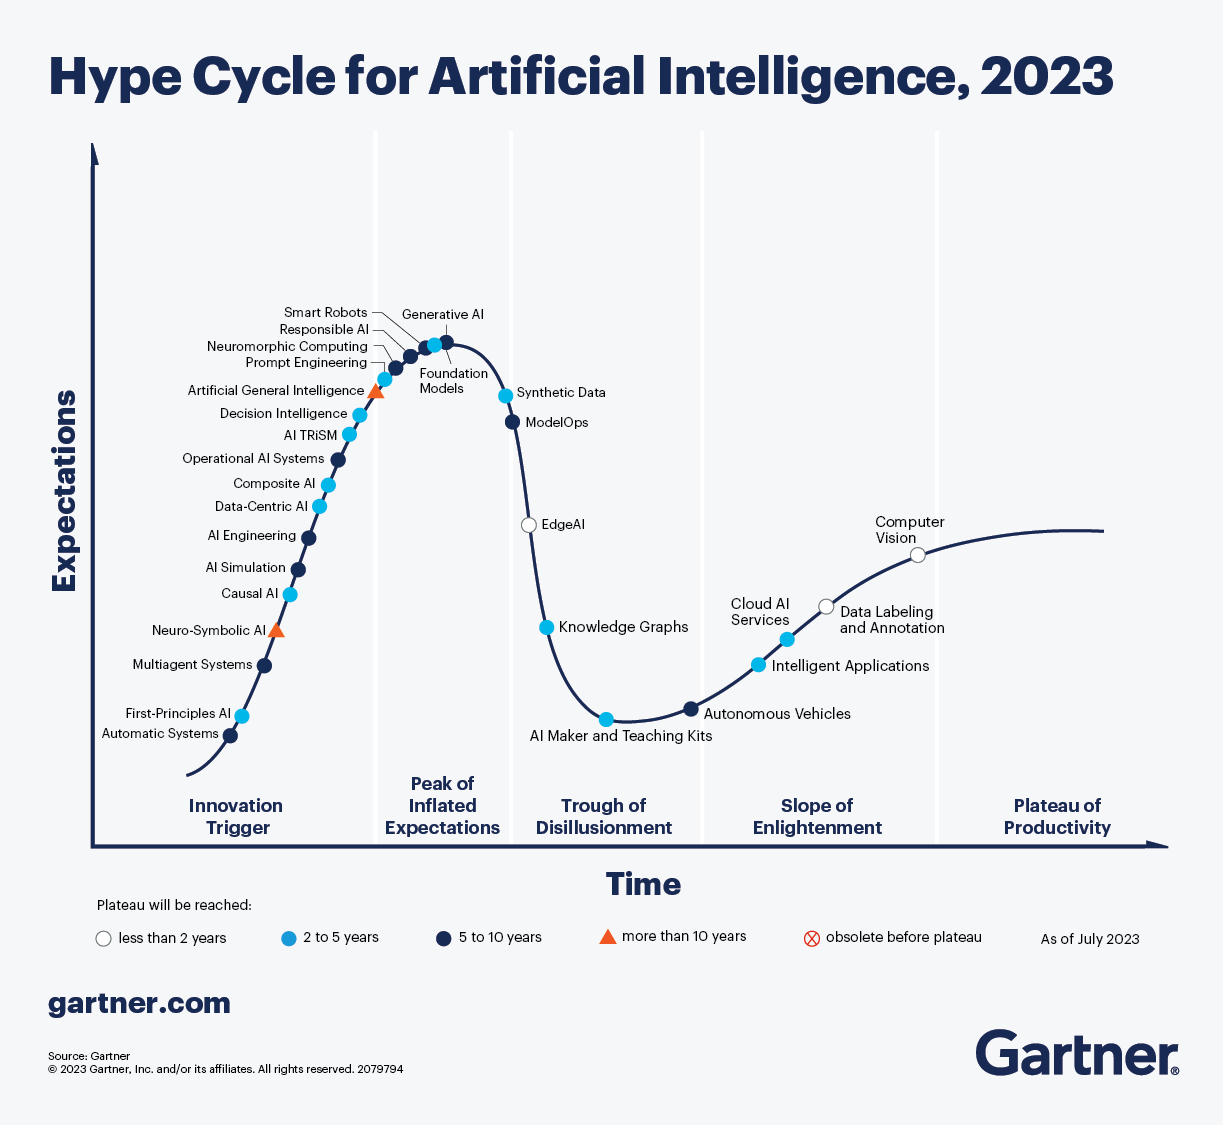
\includegraphics[width=\textwidth]{fig/intro/Gartner_2023.png}
    \caption{Gartner's 2023 hype chart for artificial intelligence.}
    \label{fig:garter-chart}
\end{figure}

The Garter institution places Knowledge Graphs in the middle of their life cycle (cf. Figure \ref{fig:garter-chart}) meaning that they can still benefit from active research and development and are still in their infancy in regard to their widespread applications in a multitude of fields. Some of the most notable fields and Knowledge Graphs corresponding to each of them are:
\begin{itemize}
    \item \textbf{Enciclopedic} KGs compile factual knowledge facts or events sourced from different domains. Some examples are DBpedia\cite{auer2007dbpedia} which compiles the knowledge found in Wikipedia articles, Freebase\cite{bollacker2007freebase} which combines automatic processes from multiple sources as well as user contributions to wrangle up its data or YAGO\cite{suchanek2007yago} which adds a layer of complexity by adding temporal and geographical information to Wikipedia facts.
    \item \textbf{Linguistic} KGs compile facts about language and add a layer of information in the form of ontologies or external features on top. The most notable of these is WordNet\cite{miller1995wordnet} which provides hyponym and synonym relationships between words of the English language.
    \item \textbf{Enterprise} KGs support tech sector companies in their endeavors. Knowledge graphs were originally conceived for this purpose as the Google Knowledge Graph (GKG) \cite{steiner2012adding} boasting an impressive 800 billion facts on 8 billion entities was incepted to aid in query answering. This graph compiles multi-domain information in order to rapidly respond to one of the many user queries made through their browser per day. 
    
\end{itemize}

Knowledge Graph construction is generally an automatic task since the large volume of data they hold extends past the range of human processing abilities without it being an exceptionally tedious, long, and costly process, however, there are some notable exceptions such as the high-quality datasets that were constructed through crowdfunding efforts such as Freebase\cite{bollacker2007freebase} and Wikidata\cite{vrandevcic2014wikidata}. Automatic KG construction typically relies on semi-structured\cite{lehmann2015dbpedia} information ranging from XML-type documents and HTML tables to plain text articles with a well-organized title structure.
The data extraction process has evolved over time, from information extraction systems driven by designated rules or clustering \cite{yates2007textrunner, etzioni2004web}, to the current approaches such as entity recognition\cite{huang2015bidirectional, ma2016end}, typing\cite{xu2018neural, ren2016label} and linking\cite{ganea2017deep, le2018improving} or relation extraction and curation\cite{zeng2015distant, zhou2016attention}. 

These methods of automated construction allow for a massive volume of data to be processed, however, they present several limitations.
First, the information they are built upon may be interpreted and linked erroneously or simply by being demonstrably wrong \cite{martinez2020information}, leading to incorrect facts being present in a KG. 
Second, Knowledge Graphs built from the same source might not be equal rendering them incompatible, they could represent the same facts with different nomenclature because they used a different schema to link that information \cite{choi2006survey}, meaning that integrating Knowledge Graphs is never a trivial task.
Finally, Knowledge Graphs constructed in this manner will most likely be lacking information that was originally contained within the source material it used \cite{bordes2014constructing}. In addition, information sources generally do not include knowledge that the intended reader should already be aware of, in other words, no source will explicitly hold all information required for a single domain, therefore, Knowledge Graphs inherently lack triples that could otherwise exist in them.
Some techniques aim to fill this information gap in automatically constructed Knowledge Graphs, known as KG completion, and their focus is on finding links between existing entities that are not present in the KG but should be. However, KG completion efforts have a limitation shared by multiple binary classifiers in the literature, they generally provide an answer to a query that can be accompanied by a degree of confidence in the form of a percentage. This lack of explainability of their answers is a limitation in KG completion that KG reasoning aims to complement by providing reasoned paths to accompany their responses. In this way, a provided answer can be human-friendly as well as serve the same purpose in regards to KG completion.

Existing literature displays the multiple ways in which KG completion and reasoning have been tackled. Completion efforts can be separated into one of four existing categories\cite{shen2022comprehensive}, they are as follows.
\textbf{Semantic matching models}, compute a scoring function by measuring the semantic similarities of entity or relation embeddings in latent embedding space, they do so by applying \textbf{Neural Network} or \textbf{Tensor Factorization} models. 
NN models \cite{socher2013reasoning, tran2020multi} present a challenging problem as they require the effective encoding of world knowledge using powerful models that try to approximate human cognition by replicating the neural structures found in our brains. Research has shown that neural networks can capture the semantic features of entities and relations intelligently and model the semantic relationships between discrete entities, ultimately leading to more accurate embeddings of KGs.
Tensors\cite{nickel2011three, balavzevic2019tucker, socher2013reasoning, } and their decompositions are widely used in data mining and machine learning problems. their usefulness comes from the representation they offer as KG entities and triples can be represented as tensors, KG completion can be tackled as a binary tensor completion problem\cite{shen2022comprehensive}.

\textbf{Translational models}\cite{bordes2013translating, wang2014knowledge, lin2015learning, sun2019rotate, trouillon2016complex, dettmers2018conve} encode KG entities and relations as low-dimensional numerical vectors. a distance scoring function is then applied in the N-dimensional vectorial space reflecting the correctness of a proposed triple, then a ranking loss function is applied to learn the top translation relation between the entities in question.
\textbf{Structural models}\cite{mikolov2013efficient, pennington2014glove} The inherent rich information inside KGs plays an important role in capturing useful features of knowledge embeddings for KG completion. the common internal information inside KGs includes node attribute information, entity-related information, relation-related information, neighborhood information, and relational path Information. This dissertation's proposal expands on relational path reasoning combined with translational elements as part of the contribution.

% This needs to be formalized, cited, completed and improved...

Obtaining information from relational paths contained within a KG is usually performed by applying machine learning algorithms; path capture, path classification\cite{xiong2017deeppath}, path augmentation\cite{manchanda2023metapath, hirose2021transductive} or multi-hop KG reasoning\cite{lin2018multi, tiwari2021dapath, cui2023incorporating, cui2023reinforcement}. Most of these approaches present an inherent flaw, they use a path ranking NN as a binary classifier which causes feature explosion for large KGs and lacks background information on the selected path, both of those shortcomings are solved by KG reasoning methods. That is why in our works we focused on the development of a multi-hop reasoning approach that adds explainability and prevents feature explosions for large KGs.

There are several options for the construction of artificial intelligence capable of performing KG reasoning, namely, supervised, unsupervised and reinforcement learning.

Supervised learning requires providing a golden truth in a labeled dataset, which means knowing the optimal outcome beforehand, this is useful for tasks that require classification and regression problems, predicting a value in continuous or discrete spaces. This is simply not possible for many problems in the field, in this case, it would mean obtaining the best path connecting two given nodes of a Knowledge Graph for the particular problem being solved. This would require expert knowledge and deep analysis for each of the nodes, a task which is simply unfeasible for sizeable Knowledge Graphs.

% In unsupervised learning no labeled dataset is provided it tries to learn the the underlying patterns of the problem and in this way approximate the output, however, traditional unsupervised approaches often struggle to handle the complexity of real-world knowledge graphs, especially when faced with missing or ambiguous information

Unsupervised learning operates without a labeled dataset, aiming to discern underlying patterns within a problem and approximate the output. However, traditional unsupervised methods frequently encounter challenges in managing the intricacies of real-world knowledge graphs, particularly when confronted with ambiguous or missing information.

Reinforcement learning emerges as a promising paradigm to address these limitations. RL introduces an interactive learning framework where an agent learns to navigate and interact with the knowledge graph by using it as the environment of the problem. RL algorithms can dynamically adapt their strategies, effectively dealing with the uncertainties present in an automatically constructed KG even in the absence of human supervision.

In practice Reinforcement Learning focuses on solving a stochastic gradient ascent problem in a KG reasoning scenario, that will be described in depth in chapter\ref{chap:reinforcement}, it is a policy gradient method seeking to optimize the quality of the found path based on the metrics of some reward functions. 

It does so by traversing through the graph nodes as states by using connected relations as the action space for that state. the objective of the Agent is to learn the best path that answers a particular query. This query can be interpreted in the form of a question that needs answering, such as, who is the partner of Keanu Reeves? This, in the KG nomenclature, is expressed as a triple missing its end node (Keanu Reeves, is\_partner\_of, ?), the agent is then expected to find the destination node while training in order to generate new paths of information from the unanswered queries contained in the KG.

Several proposals have tackled this problem in the past \cite{xiong2017deeppath, das2017go, lin2018multi, xian2019reinforcement} however they present several shortcomings, for instance, they require the embedding models to be computed before attempting the problem. Also, they restrict themselves to using classical RL backpropagation algorithms and overlook the application of more modern options such as Proximal Policy Optimization (PPO)\cite{schulman2017proximal} or Soft Actor-Critic (SAC) \cite{haarnoja2018soft} while also relying on simple reward structures. Finally, most of these proposals are not distributed as usable tools intended for final users. Even if they make their implementation publicly available, their code is generally intended for the sake of reproducibility of their experimental results, and they often lack any degree of customization or flexibility, meaning they usually can only work on a number of predefined datasets as input.

In this dissertation work, we aim to combine the benefits from RL pathfinding with the power of representational embeddings to infer fairly long and explainable paths, useful for KG-based applications, and it can do so with on-the-fly embedding generation and embedding-based rewards combined with step-based rewards.

The tool presented is highly configurable, allowing for reward calculation to be modified with a combination of several options, customizing the policy intermediate activation function and regularization and allowing the user to apply state-of-the-art RL algorithms out of the box, which improves performance and helps avoid reward plateaus while training.

Finally, we aim to provide a versatile tool intended for users with different levels of expertise, from novices to experts. It allows comprehensive and flexible customization for advanced users, who may prefer to install SpaceRL as a server for their local usage or to become a service provider for third parties. On the other hand, it also offers a simple MLaaS interface, intended for a more untrained end user. Machine Learning as a Service (MLaaS) has gained traction in recent years since it adds layers of abstraction that create a black-box simplified interface for a non-expert final user. SpaceRL offers RL model generation and usage as a service capability, either locally through its GUI or as a deployable REST API for third-party consumption. Therefore, it is, to the best of our knowledge, the first turnkey tool to provide such RL KG completion and reasoning functionalities.

\section{Research rationale}\label{sec:intro-rationale}
In this section, we present the hypothesis that has motivated our research work in the context of Knowledge Graph reasoning and state our thesis, which we prove in the rest of the dissertation.

\subsection{Hypothesis}
\todo{En mi opinion aqui no solo debemos hablar de la oportunidad que suponen los grafos de conocimiento como tal y por eso hay que completarlos, si no de lo que supone mejorar la accesibilidad de las prpuestas que lo ofrecen, porque tambien forma parte de la tesis, no creo por tanto que la mencion a la limitacion de las técnicas sobre de aqui.}

Currently, Knowledge Graphs present a tantalizing alternative for structuring information about one or multiple domains. They offer a semantic connection between the data nodes which can be used for a multitude of applications such as question answering \cite{cui2023incorporating, cui2023reinforcement}, recommendation systems \cite{xian2019reinforcement}, biomedical studies \cite{nicholson2020constructing} or natural language processing tasks. The nature of these knowledge graphs makes them inherently incomplete as their construction is often automatic, granting for their expansion with a variety of techniques. 
however, these techniques \cite{bordes2013translating, wang2014knowledge, lin2015learning, sun2019rotate, trouillon2016complex, nickel2011three, balavzevic2019tucker, socher2013reasoning, lao2011random, das2017go, xiong2017deeppath, lin2018multi, xian2019reinforcement, tiwari2021dapath} come with their own set of limitations, most notably how they provide close to no input about why they provided the results they did. In addition, the tools available to perform these tasks are limited due to the nature of their conception, created to test a specific technique and made available for replication purposes only by expert users, as opposed to being designed with usability and customization in mind.

According to the previous argumentation, we conclude that our hypothesis is the following:

% Knowledge Graphs provide value to individuals and companies alike by supporting applications that are widely used today, and their usefulness is likely to keep growing. Due to their incompleteness, there is a need to refine them and find the information that they are missing in order to expand them.

\hypthesis{Knowledge Graphs provide a way to structure information such that it provides semantic value to applications that rely on them and are widely used. They are inherently incomplete and can be expanded, however the methods that can do so are limited in two major ways, they lack explainability on the knowledge generated and are offered for expert users only, if at all.}

\subsection{Thesis}

\todo{estoy de acuerdo en que esto le falta contexto en algun momento, lo reescribiré.}

A multitude of approaches have tackled the problem of KG completion \cite{} and reasoning \cite{}, however, triple classification KG completion approaches lack explainability for their results and can not provide any knowledge past the inclusion of new triples with a certain degree of confidence. KG reasoning approaches do provide a degree of explainability for their results and they do so based on algorithms and techniques that are limited due to their reward structures based on retropropagating simple terminal rewards and their highly variable inference due to the RL algorithms used, even disregarding the semantic value of the embeddings they use for representation of the different states. These techniques could be updated or expanded if their methods were aimed towards this goal, however, the tools presented by them are almost always tailored for the only purpose of producing results for publication and nothing more, this generally means making them hard to work with and even harder to expand them.

In light of the previous reasoning, we conclude that our thesis is as follows:

% In the context of Knowledge Graph completion, it is possible to overcome the problems of existing proposals and develop a new one to automatically complete the missing information in a large KG, in a way that does not rely on external information or alternative representations, but that still achieves a high effectiveness.

\hypthesis{Knowledge graph reasoning can benefit from the development of novel reward structures that leverage the semantic value contained within the embedding representations of graph nodes and relations, more robust Reinforcement Learning algorithms that circumvent the high variance of the methodology of policy gradient methods and from a standardized approach to applying these techniques that focuses on ease of expansion and modification for the purpose of making it possible to implement new techniques in the future.}

\section{Summary of contributions}\label{sec:intro-summary}
To prove our thesis, we have devised \href{https://github.com/DEAL-US/SpaceRL-KG}{\textbf{\textit{SpaceRL our KG reasoning framework}}} supported by Reinforcement Learning techniques.

SpaceRL is an end-to-end framework focused on customization and adaptability, it works with any dataset provided in the expected format. SpaceRL allows any user with any level of expertise to generate an intelligent agent able to reason over the KG of their choice in order to generate new knowledge in the form of a triple accompanied by a structured reasoned path.

The framework allows the users to customize it by permitting the tuning of hyperparameters, relying on previous experience with LSTM layers, generating a particular set of embeddings for the dataset being used, using multiple RL algorithms, reward structures and depth of reasoned paths.

It also allows for the deployment of a relation API in order to be a service provider for tuned models or to provide infrastructure for model generation to a third party, as well as offering a GUI in order to give inexperienced users a comprehensive view of the system for them to generate models and tune them as needed, without expert knowledge of the field. The system also offers visualization tools that give the user an overview of how the trained models choose the paths while in inference mode in order to better understand the decisions made.

SpaceRL is meant to be easily expanded, however, it also comes with multiple options out of the box, we have mentioned in the introduction how current KG reasoning approaches are lacking in inference stability, which is why SpaceRL defaults to the usage of the Proximal Policy Optimization (PPO) reinforcement learning algorithm and comes out of the box with novel reward structures based on the properties of the embeddings for the evaluated KG. these options were used in our paper "SpaceRL-KG: Searching Paths Automatically Combining Embedding-based Rewards with Reinforcement Learning in Knowledge Graphs", currently under review in Expert systems with applications. The framework, complete with API and GUI has been sent to SoftwareX, and is currently awaiting to be reviewed by the editor.

\section{Structure of this dissertation}\label{sec:intro-structure}
This dissertation is structured as follows:

\begin{description}
    \item[\textbf{Part I: Preface.}] 
    It holds the introductory chapters to this dissertation, the one holding these words plus Chapter \ref{chap:motivation}, where we go into detail about the justification that granted the works presented in this book, presenting the limitations of the current state-of-the-art approaches\\
    
    \item[Part II: Background Information.] 
    This section gives insight into the topics necessary to better understand the proposals presented, In chapter \ref{chap:kgs} we give an overview of Knowledge graphs, how they are structured, constructed, applied and the challenges in the field. In chapter \ref{chap:embeddings}, we introduce the representational techniques for knowledge graphs known as embeddings, how they work and several proposals that apply the different techniques used to generate them. In chapter \ref{chap:reinforcement} we give an introduction to Reinforcement Learning, how it can solve KG reasoning tasks and how it operates within the scope of a knowledge graph, the evolution of the techniques and algorithms and how each of them operates and some applications RL has had success on.
    
    \item[Part III: Our Proposal.]
    This section reports on the contributions made to this dissertation. In chapter \ref{chap:SpaceRL} we describe the methodology followed to create reinforcement learning agents and how they fared on several state-of-the-art datasets to generate reasoned paths following our new reward structure and use of modern RL algorithms. In chapter \ref{chap:framework} we present our framework for RL-based KG reasoning tasks, how it works and the advantages it poses over creating new one-time use code for a proposal, how it can help expert users provide a service to others and how can be used by non-expert users.
    
    \item[Part IV: Final Remarks.]
    It contains Chapter~\ref{chap:conclusions}, which concludes this dissertation and presents some possible future research directions.
\end{description}
    \chapter{Motivation}\label{chap:motivation}

\chapterQuote{\textit{``The worthwhile problems are the ones you can really solve or help solve, the ones you can really contribute something to. No problem is too small or too trivial if we can really do something about it.''}}{--- Richard Feynman}

\chapterAbstract{D}{}

% espite Knowledge Graph completion being a very active research topic, the current proposals for carrying it out still have some drawbacks that hinder their applicability in practice, and which should be solved. Our goal in this chapter is to present the problems that arise in practice when completing Knowledge Graphs, and to motivate the need for a new proposal. This chapter is organized as follows: Section~\ref{sec:moti-intro} introduces it and provides the necessary background knowledge, Section~\ref{sec:moti-problems} presents the problems of KG completion in detail, Section~\ref{sec:moti-analysis} analyzes the current approaches and their main problems, Section~\ref{sec:moti-discussion} explains how none of the existing proposals solves all practical problems at a time, Section~\ref{sec:moti-proposal} introduces our contributions and compares them with the existing proposals in the literature; finally, Section~\ref{sec:moti-summary} summarizes the chapter.



\section{Introduction}\label{sec:moti-intro}
\begin{itemize}
    \item Increase in interest by companies like google amazon etc\dots
    \item they are good for organization of information
    \item they need to be as complete as possible
    \item they need to be organized in such a way that the answers they provide have an explanation (explainability)
\end{itemize}
% Nowadays, there is an increasing interest of individuals, organizations and
% companies in Knowledge Graphs, in order to organize, store and publish their data. This, in turn, can support many practical applications in a variety of domains, such as commerce \cite{zhang2021, palumbo2020}, education \cite{chen2018, aliyu2020}, research \cite{wang2018, dessi2020aikg, dessi2022cskg}, or healthcare \cite{zhang2020b, gong2021, wise2020}, to cite a few.

% Ideally, these Knowledge Graphs should be as complete as possible, to make sure that they include all pieces of knowledge that may be relevant to the organization that manages it or the users they support. However, due to the way in which they are constructed, it is well-known that this is not the case \cite{paulheim2017,shen2022overview,hogan2020,peng2023}. Those that are automatically built from external knowledge sources rely on the completeness of the original source and the capabilities of automated information extractors, which are far from perfect \cite{mitchell2018, bordes2014b}. Additionally, KGs that are built manually, either by their creators or by a crowdsourced process, tend to be much smaller in size \cite{miller1995}. Due to these reasons, there exists a large number of incomplete KGs under active use today, and a need to complete them \cite{shrivastava2017, krishnan2018, pittman2017, noy2019, singhal2012}.

% In the literature, there are different proposals to address the problem of
% completing Knowledge Graphs, e.g., \cite{jiang2016, galarraga2015, wang2015, kuzelka2019, yang2017, sadeghian2019, minervini2018, wei2015, garcia-duran2015, yang2014, tay2017, trouillon2016, lin2015, do2018, gardner2015, nastase2019, gu2015, toutanova2016, jiang2017, lei2019, bansal2019a2n, wang2019}. Unfortunately, these proposals have a number of drawbacks that hinder their applicability in practice. Consequently, it is still necessary to research on the field of Knowledge Graph completion, which is our purpose in this dissertation.

\section{Problems}\label{sec:moti-problems}
\begin{itemize}
    \item They require embeddings to work.
    \item Only specific solutions exist for a particular approach (no general purpose)(no open source).
    \item little to no reason of included information (low explainability)
    \item something something reinforcement learning?
\end{itemize}
% Completing Knowledge Graphs is not a trivial task and, if not performed correctly, it may reduce the quality of the knowledge contained in them. In this section, we present the problems that must be addressed by proposals that perform this task in order to be useful in practice. These problems are as follows:

% \begin{description}
    % \item[(P1) To rely on embedded representations of entities and/or relations:] Many of the current proposals rely on generating, or being provided with, embedded representations of the entities and/or relations in a Knowledge Graph. These embedded representations are more compact versions of the elements they represent, usually as a vector that encodes the position of an entity or relation in an N-dimensional space. Embedded representations can be useful because they can capture meaningful semantic similarities between different elements, however, their use hinders the practical application of a proposal. Those proposals that require that embedded representations be provided to them are no longer stand-alone, they instead have a strong dependence with the tools that generates the embeddings and the quality of them. Even those that generate them themselves suffer from another issue: the need to completely remake them ---incurring in a very high computational cost--- whenever a new entity or relation is added to the KG, which is an event that tends to happen frequently \cite{mitchell2018,dong2014}. \\
    
    % \item[(P2) To depend on external sources of information:] An external source of information can be a structured or semi-structured repository of information, an information retrieval or query system, another Knowledge Graph or, in general any means for automatically accessing information besides the Knowledge Graph that is to be completed. Depending on these external sources introduces a single point of failure in the KG completion process that is not admissible in many practical and commercial applications. Furthermore, depending on the nature of the information source, its contents or means of access may change without any previous warning, rendering the KG completion proposal ineffective or, at least, requiring extensive maintenance.\\
    
    % \item[(P3) To need user-provided data or supervision:] Knowledge Graphs can store large amounts of information; some of the most well-known KGs used nowadays contain millions of triples, and some of them can reach even higher orders of magnitude \cite{singhal2012}. For this reason, it is not reasonable to rely on any sort of human-provided information in order to complete them. The required volume of human input for a standard Knowledge Graph would be unattainable for just a few human experts, and using a crowdsourcing process would greatly decrease the quality of the information that is fed to the KG completion process.\\
    
    % \item[(P4) To not have any means to automatically generate new knowledge:] Many of the existing KG completion proposals in the literature are able to determine whether a triple is correct or not, which is undoubtedly an important step, but they do not have any mechanisms to autonomously generate new knowledge. Instead, they rely on a set of possible facts being passed on to them for evaluation, but they do not specify how this set of facts should be created. Other proposals have a limited way to do this, by suggesting which entities are more likely to appear in a triple along with another given entity and relation. Although it is an improvement, it is still not practical to assess all possible pairs of entities and relations in a KG.\\
    
    % \newpage%\todo{quitar?}
    % \item[(P5) To not be applicable to large Knowledge Graphs:] As mentioned previously, most Knowledge Graphs contain large volumes of information. Even if a proposal relies entirely on information present in the graph, some of them use approaches that are known not to be scalable enough to be applied to some of the most popular Knowledge Graphs available nowadays.\\

% \end{description}

\section{Analysis of current solutions}\label{sec:moti-analysis}

Here add some tables similar to the ones already presented in ohter papers which evaluate multiple proposals in the topic, then compare why these approaches are not complete and why ours makes strides towards filling the gaps.

Most notably, terminal rewards and retropropagation, use of REINFORCE algorithm, little in the way of Actor-Critic approaches, precomputation and lack of usability.

An enumeration of references is also a possibility for this section, adding the benefits of each proposal in an incremental way and what they are missing.

% There already exist a number of proposals for completing Knowledge Graphs in the literature. In Table~\ref{table:proposals}, we summarize them and the problems they suffer from, and in the following, we discuss them in more detail:

% \begin{table}[!htp]
    \begin{center}
        \renewcommand{\arraystretch}{2.0}
    \begin{tabular}{>{\raggedright\arraybackslash} M{5cm} | M{1cm} | M{1cm} |  M{1cm} |  M{1cm} |  M{1cm}}
    
    \specialrule{1.2pt}{3pt}{3pt}
    \centering \textbf{Proposal} & \textbf{P1} & \textbf{P2} & \textbf{P3} & \textbf{P4} & \textbf{P5}  \\
    \specialrule{1.2pt}{3pt}{3pt}

    \citet{bordes2013} & \no & \yes & \yes & \no & \yes \\ \hline % TransE 
    \citet{galarraga2015} & \yes & \yes & \yes & \yes & \no \\ \hline % AMIE
    \citet{gardner2015} & \yes & \yes & \no & \no & \yes \\ \hline  % SFE
    \citet{guo2016} & \no & \yes & \no & \no & \yes \\ \hline  % KALE
    \citet{jiang2016}& \yes & \no & \yes & \yes & \no \\ \hline % ILP
    \citet{kazemi2018} & \no & \yes & \yes & \no & \yes \\ \hline % SimplE
    \citet{lao2011} & \yes & \yes & \yes & \no & \yes \\ \hline % PRA
    \citet{lin2015} & \no & \yes & \yes & \no & \yes \\ \hline % TransR
    
    \citet{nickel2011} & \no & \yes & \yes & \yes & \no \\ \hline % RESCAL
    \citet{shi18} & \no & \no & \yes & \yes & \yes \\ \hline % ConMask
    \citet{trouillon2016} & \no & \yes & \yes & \yes & \no \\ \hline % ComplEx
    
    \citet{wang2014} & \no & \yes & \yes & \no & \yes \\% TransH
    \specialrule{1.2pt}{3pt}{3pt}
    
    
    
    
    
    
    



    \end{tabular}

    \vspace{.5cm}
    {
        \flushleft
        P1 = To rely on embedded representations of entities and/or relations; P2 = To depend on external sources of information; P3 = To need user-provided data or supervision; P4 = To not have any means to automatically generate new knowledge; P5 = To not be applicable to large Knowledge Graphs.\\
        
        \flushleft
        A \yes{} means that the proposal is free from a problem, while \no{} means that it is present.
    }

    \caption{Comparison of current proposals for KG completion}
    \label{table:proposals}
    \end{center}
\end{table}

% \citet{bordes2013} devised a proposal that learns embedded representations of the entities in a Knowledge Graph, in order to place them in an N-dimensional space while transforming semantical similarities into physical closeness in said space. In this proposal, the correctness of a triple can be checked by evaluating the relative positions of its two entities in the embedded space.

% \citet{galarraga2015} proposed a rule extractor that is able to capture common patterns in a Knowledge Graph using Inductive Logic Programming (ILP), and express them using first-order rules. Once these rules have been mined, they can be applied to materialize new knowledge in the KG.

% \citet{gardner2015} introduced a technique that defines a series of features to characterize the path between two entities, and then analyzes a large number of said paths to learn to identify a possible direct connection between the entities. However, it requires the manual introduction of an ``Alias'' relation, which indicates that two entities in a KG refer to the same concept in the real world.

% \citet{guo2016} presented a proposal that combines the use of entity embeddings and logical rules. It provides a shared framework in which rules and embeddings can directly interact with each other. This is done by representing the triples in a KG mathematically, and defining a series of operators. The semantic information present in the entity embeddings helps expand the predictive capabilities of the rules that this proposal produces.

% \citet{jiang2016} proposed another approach that uses ILP to find and exploit rules in a Knowledge Graph, more particularly, by analyzing the intervals of validity of the facts contained within it and reasoning when other related facts will start or stop being valid. This requires the introduction of temporal annotations in the KG which, generally, must be manually provided.

% \citet{kazemi2018} also leverage entity and relation embeddings, and propose adding an extra inverse relation for every one that is already present in a KG. This allows their proposal to reach a higher degree of expressivity, while its simple embedding model allows it to be applied to large KGs.

% \citet{lao2011} presented a technique that uses random walks to traverse the space in the KG between the two entities of a triple. By analyzing examples of correct and incorrect triples, their proposal is able to learn whether two entities should be connected according to the possible paths that can be traced between them.

% \citet{lin2015} proposed a different use of embedding spaces, by defining two groups of them, one exclusively for entities and one for every different relation present in a KG. Their model is able to express triples as transformations between relation spaces through the use of projection matrices. The increased number of embedding spaces makes it more computationally complex, but also more effective.

% \citet{nickel2011} suggested using tensors to represent a Knowledge Graph, and then factorizing those tensors to obtain more compact representations of the knowledge in them. Their approach works by using a third-order binary tensor that holds information about which entities are connected in the graph and through which relation, and then performing a series of mathematical operations that result in another tensor, with confidence levels for any possible fact that could be introduced in the KG, given its current entities and relations. However, the size of the tensor scales quadratically with respect to the number of entities, making it a poor choice for large KGs.

% \citet{shi18} introduced a proposal that uses not only the embeddings of an entity, but also of its textual description, to look for additional levels of semantic similarity. Additionally, their proposal does not rely on generating negative examples, like most other existing state-of-the-art proposals do. However, it relies on external sources of information to retrieve the descriptions of the entities.

% \citet{trouillon2016} proposed a technique that factorizes the tensor representation of a KG, but instead of binary values, it uses complex numbers. This can be seen as generating two separate tensors: one which contains the real parts of the values, and another one that contains the imaginary parts. The usage of complex numbers allows it to simplify some of its internal calculations, making it slightly more efficient.

% \citet{wang2014} proposed using translation on hyperplanes to change the embedded representation of an entity, depending on which relation is being used to link it with another entity. However, these translations, just like the overall embedding space, must be re-learned whenever a change in the KG occurs.

\section{Discussion}\label{sec:moti-discussion}

This section is not on both Agu's and Inma's thesis(es?), a mixed approach is best I believe, present a table that evaluate each of the proposals shortcomings and a brief explanation for each of them is also good.

In summary remove this section and provide all information on the previous one.
% The previous proposals have problems that hinder their applicability in practice. Regarding the use of embeddings (P1), most of the existing KG completion techniques in the literature rely on them to some extent \cite{bordes2013,guo2016,kazemi2018,lin2015,nickel2011,shi18,trouillon2016,wang2014}. This is problematic because, as discussed, most KGs are in constant expansion, and adding any entity or relation to the KG must trigger a re-computation of said embeddings, which is not feasible in practice.

% \citet{jiang2016} and \citet{shi18} propose techniques that depend on outside information (P2), making them vulnerable to changes in the sources of external information. Furthermore, the proposals made by \citet{gardner2015} and \citet{guo2016} are not fully automated, and require manual intervention by the users (P3).

% Regarding the automated generation of new knowledge (P4), there are few techniques that are able to do it independently. The approaches proposed by \citet{galarraga2015} and \citet{jiang2016} provide a straight-forward way to achieve this, since they generate first-order logical rules that can be used to materialize new knowledge in the KG. The tensor factorization approaches introduced by \citet{nickel2011} and \citet{trouillon2016} also enable this by traversing the resulting tensor, which contains confidence scores for all possible facts, and adding those whose score exceeds a certain threshold (although this may be time-consuming given the size of the tensors). Finally, \citet{shi18} use a simplified way of generating candidate triples, by generating and examining those in which the left-hand entity and relation already appear together somewhere else in the KG.

% Most existing proposals can be applied to large Knowledge Graphs (P5), although there are some exceptions. The proposals made by \citet{galarraga2015} and \citet{jiang2016} rely upon rule mining through ILP, which is known to scale poorly to large collections of facts \cite{shen2022overview}. Additionally, tensor factorization techniques, such as those proposed by \citet{nickel2011} and \citet{trouillon2016}, need to generate tensors that contain $R \cdot E^2$ elements, where $R$ is the number of distinct relations in a KG and $E$ is the amount of different entities. This size can quickly become unmanageable when the KG contains more than a few thousand entities.

\section{Our proposal}\label{sec:moti-proposal}
In this dissertation, we present a proposal for Knowledge Graph reasoning SpaceRL which...


% To determine the correctness of a triple, we introduce CAFE, our triple classification technique. It relies solely on path and entity neighborhood information present in the graph, which, contrary to embeddings, does not require any pre-computation or significant re-generation when the graph changes (P1). It is also able to operate taking only a Knowledge Graph as input, without any additional dependencies on external sources of information (P2). CAFE works by transforming the triples in a KG into a set of labeled feature vectors, using a novel set of context-aware features, and then learning to differentiate between correct and incorrect triples in a completely automated manner, without any user intervention (P3).

% We also present CHAI, our proposal for automatically generating candidate triples. CHAI is able to materialize sets of possible facts of a reasonable size, that include most of the information that is missing in a KG. These facts can be passed on to a triple classification technique such as CAFE, thus solving the problem of generating new knowledge (P4).

% Finally, to prove the applicability of our proposal, we introduce SciCheck, an extension of CAFE specifically tailored to scientific Knowledge Graphs. We show that SciCheck can be applied to AI-KG, a large scientific KG with over 14 million triples, yielding very satisfactory results and taking considerably less time than other existing approaches in the literature (P5).

\section{Summary}\label{sec:moti-summary}
Summary of section.
% In this chapter, we have motivated the reason for this dissertation. We have analyzed the problems of completing Knowledge Graphs and the current proposals in the literature to carry out this task, and we have concluded that none of these proposals solves all of the presented problems at a time.

    %%%%%%%%%%%%%%%%%%%%%%%%%%%%%%%%%%%%%%%%

    \part{Background Information}
    \chapter{Knowledge Graphs}\label{chap:kgs}

\chapterQuote{\hfill\textit{``To know that we know what we know, and to know that we do not know what we do not know, that is true knowledge.''}}{--- \textit{Nicolaus Copernicus}}

\chapterAbstract{K}{nowledge Graphs (KGs) are a way to structure information by representing them into a series of interconnected facts and relations between them. This chapter gives some context around them. It is divided into the following sections: Section~\ref{sec:kgs-intro} presents a brief history of Knowledge Graphs and their adoption. Section~\ref{sec:kgs-current} goes over some of the more relevant KGs currently. Section~\ref{sec:kgs-applications} goes about some of the many applications KGs are currently being used for. Section~\ref{sec:kgs-challenges} reflects the current open challenges for KGs. Finally, Section~\ref{sec:kgs-summary} summarizes and concludes this chapter.}


\section{Introduction}\label{sec:kgs-intro}
% METER ESTA IDEA AQUI.
% Es gracioso que los grafos de conocimiento al fin y al cabo no representan nada "nuevo" ya que una base de datos relacional puede implementar grafos etc. Se puede mencionar la idea de que los grafos de conocimiento permiten quitar bagaje y tener algo simple de implementar, expandir, y al que aplicar algoritmos.

Before the emergence of knowledge graphs, information was predominantly stored in traditional databases and represented in tabular formats. While these databases were effective at storing structured data, they lacked the capacity to capture the complex relationships and semantics inherent in real-world information.

The concept of knowledge graphs can be traced back to the early days of Artificial Intelligence (AI) research. In the 1960s and 1970s, researchers began exploring methods to represent knowledge in a form that could be understood and utilized by computers. Early endeavors focused on semantic networks, which used nodes to represent concepts and edges to denote relationships between them.

The advent of the World Wide Web in the 1990s brought about an explosion of digital information. As the volume of web content grew, so did the need for more sophisticated methods of organizing and extracting knowledge from this vast repository. This led to the development of the Semantic Web, a vision championed by Sir Tim Berners-Lee, which aimed to make web content machine-understandable.

A pivotal milestone in the evolution of knowledge graphs was the introduction of the Resource Description Framework (RDF) in the late 1990s. RDF provided a standardized way to describe resources on the web and establish links between them. This laid the foundation for the creation of linked data, which allows for the interconnection of disparate datasets on the web.

In 2012, Google introduced the term "Knowledge Graph" as a central element of their search engine. Google's Knowledge Graph aimed to enhance search results by providing contextual information about entities and their relationships. This marked a significant shift towards a more semantically enriched approach to information retrieval.

Rather than a simple collection of relations between names of entities, they started to be seen as a rich, interconnected structure of elements (\textit{``things, not strings''}) with an enormous potential for practical and commercial applications. Many other large companies the likes of Amazon, Facebook, Microsoft and eBay soon followed suit 
% \cite{shrivastava2017, krishnan2018, pittman2017, noy2019},
and the term Knowledge Graph (KG) rose to the popularity it still enjoys nowadays, replacing the denomination ``Knowledge Base''.

Today, knowledge graphs have become a cornerstone of various AI applications, including natural language processing, recommendation systems, and data integration. Their ability to represent complex relationships and semantic context has made them an invaluable tool in the era of big data and advanced machine learning techniques.

% kept this here for the citations...

% Representing and storing structured domain-specific knowledge has been an active research topic since at least 1970, when the first relational databases were introduced \cite{codd1970}. Given their indisputable success, many alternative means of representing knowledge in an structured manner have been proposed over the years. One of such proposals was using what was coined as a \textit{Knowledge Base} (KB) \cite{hayes-roth1983}, a collection of facts that are stored as direct relations between concepts. Contrary to relational databases, which need to go through a normalization process that introduces a number of indirections to represent a piece of knowledge, KBs were considered more straightforward to operate and reason about \cite{russell2020}. A number of Knowledge Bases were thus created and maintained throughout the subsequent years by multiple organizations and research entities, which were both general-purpose~\cite{mahdisoltani2014,lehmann2015dbpedia, rebele2016, carlson2010, bollacker2008, vrandevcic2014} and domain-specific~\cite{chakravarty2017, thorn2013pharmgkb, wishart2009, wishart2008, kanehisa2010}.

% The information inside a Knowledge Base was stored in the form of entities, which represented real-world or domain-specific concepts, and relations that link these entities together. This is known as a triple: a combination of two entities by means of a relation, which usually contains a verb. For example, a KB can represent the fact that Magnus Carlsen is a chess player using the triple \textit{(Magnus Carlsen, plays, Chess)}. Such triples were generally encoded in a KB using the RDF/XML format \cite{decker2000}, or an extension of it called RDFS, which allows for a higher degree of expressivity. However, since RDF/XML is mainly intended for machine use, later KBs also used other formats, like N3, Turtle, or RDF/JSON, which are more human-readable.

% However, the introduction of the Google Knowledge Graph in 2012 \cite{singhal2012} was a pivotal point for both the industrial use and academic research of Knowledge Bases.


% In the following sections, we present the most popular Knowledge Graphs that are under active use today and the ways in which they are constructed. We then discuss the many practical applications that can, and have been, derived from the usage of KGs in commercial and academical contexts. However, despite their many benefits, Knowledge Graphs still present several challenges that must be addressed to improve their functionality and usefulness. Therefore, we also provide an overview of the main open challenges that need to be addressed to refine and improve Knowledge Graphs.

\section{Modern Knowledge Graphs}\label{sec:kgs-current}

% Nowadays, there are a number of popular Knowledge Graphs under active use, either commercial or academical. Some of the most prominent ones are as follows:

\begin{itemize}
    \item \textbf{DBpedia} is a community-driven knowledge graph that extracts structured information from Wikipedia articles. It covers a wide range of topics and provides structured data about entities, their attributes, and relationships. DBpedia utilizes natural language processing and information extraction techniques to parse Wikipedia articles and convert unstructured text into a structured RDF format.
    
    \begin{figure}[!h]
        \centering
        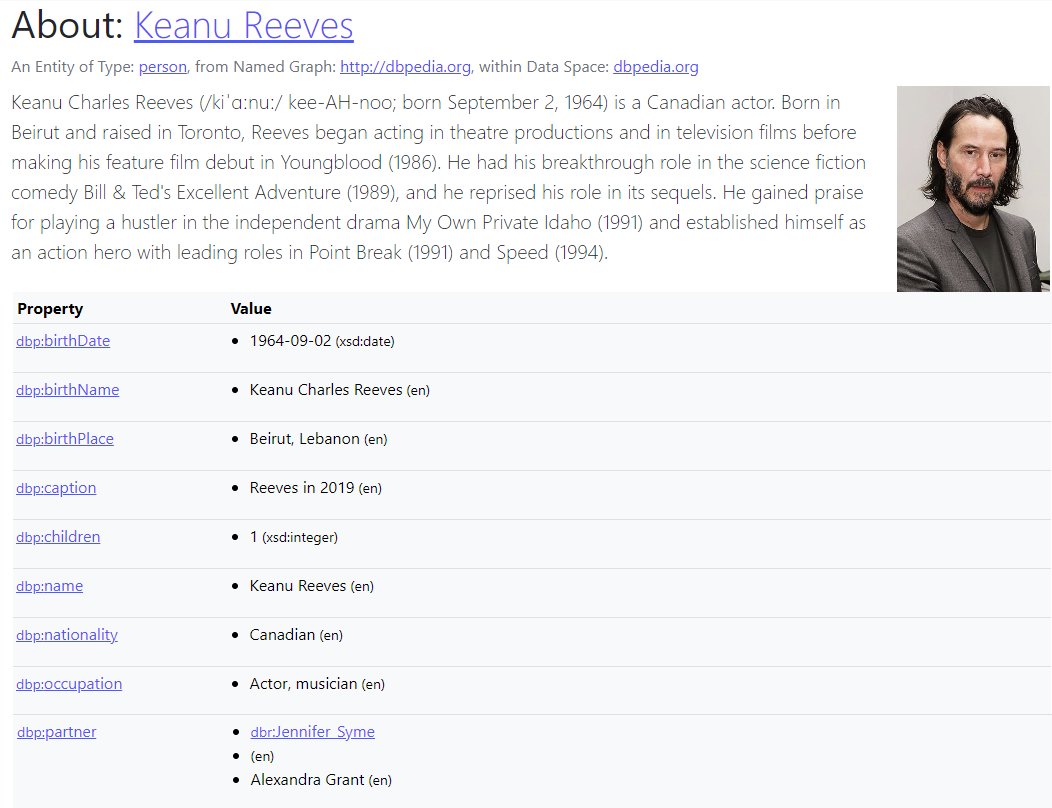
\includegraphics[width=\textwidth]{fig/kgs/Keanu_DBpedia.png}
        \caption{The ontology \textit{Keanu Reeves} in DBpedia}
        \label{fig:kgs-dbpedia}
    \end{figure}
    
    \item \textbf{YAGO} (Yet Another Great Ontology) is a knowledge graph that combines data from Wikipedia, WordNet, and GeoNames. It provides a comprehensive representation of entities and their relationships. Created using automated extraction techniques and ontological alignment to integrate information from multiple sources.
    
    \item \textbf{Wikidata} is a collaborative, multilingual knowledge graph maintained by the Wikimedia Foundation. It serves as a central repository of structured data for Wikimedia projects and beyond, containing information about a diverse set of topics it is built by a global community of volunteers who contribute, edit, and curate data using a web-based user interface.
    
    \begin{figure}[!h]
        \centering
        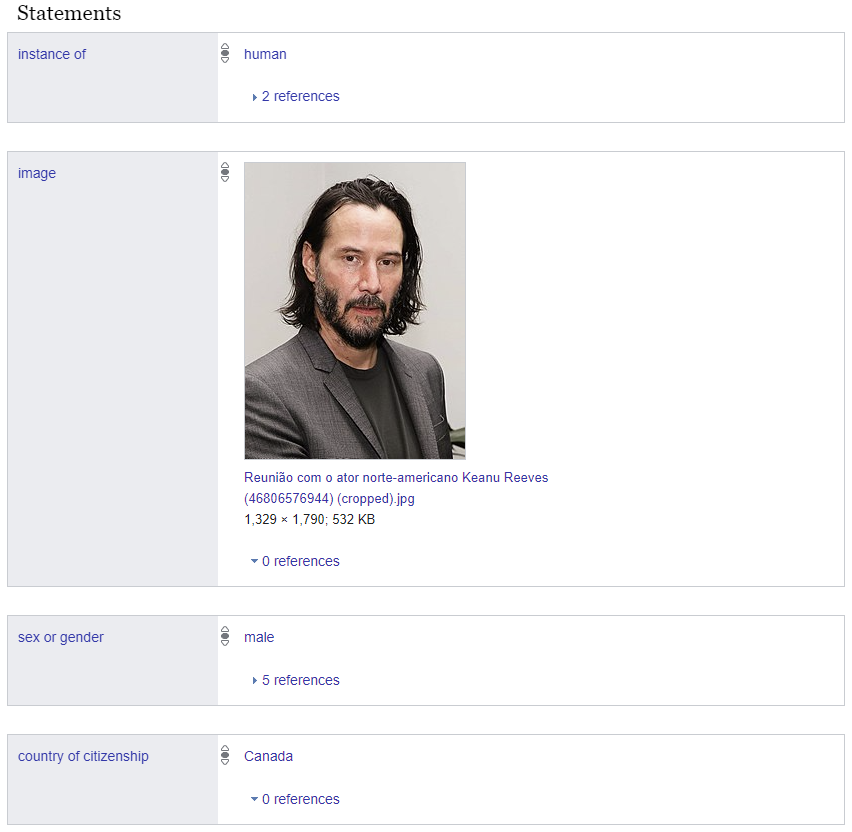
\includegraphics[width=\textwidth]{fig/kgs/Keanu_Wikidata.png}
        \caption{The entity \textit{Keanu Reeves} in Wikidata}
        \label{fig:kgs-wikidata}
    \end{figure}

    % \item \textbf{GeoNames} is a geographical database that provides detailed information about places worldwide, including countries, cities, and landmarks. It also includes coordinates and population data, it combines data from various sources, including official government databases, with user contributions and validation processes.

    \item \textbf{UMLS (Unified Medical Language System)} is a comprehensive ontology and knowledge graph for the biomedical domain. It integrates terminology and data from various biomedical sources. UMLS is built through a combination of manual curation by domain experts and automated processes for integrating and mapping different terminologies.
    
    \item \textbf{Freebase (Now Part of Wikidata)} was a large-scale knowledge graph acquired by Google in 2010 and later integrated into Wikidata. It contained structured data on a wide array of topics, including people, places, and concepts. It was constructed through a combination of automated data extraction, crowd-sourcing, and expert curation.
    
    \item \textbf{WordNet} is a lexical database of the English language, organized in a semantic network. It groups English words into sets of synonyms (synsets) and provides short, general definitions. WordNet is manually constructed by lexicographers who define word meanings and establish semantic relationships between words.
    
    \item \textbf{NELL (Never-Ending Language Learning)} is a project aimed at creating a machine learning system that continuously learns to extract structured information from the web. It aims to discover new facts about entities over time it uses a combination of natural language processing, machine learning, and information extraction techniques to learn and update its knowledge base.
\end{itemize}

\section{Applications}\label{sec:kgs-applications}

Knowledge graphs, as we explored in the preceding chapter, are structured representations of information that emphasize the interconnectedness of entities, attributes, and relationships. This section delves into the practical applications and diverse utility of knowledge graphs across a spectrum of domains. The power of knowledge graphs lies not only in their capacity to organize information but also in their ability to unlock a deeper layer of context, semantics, and relationships within data. 

They have emerged as a foundational tool in modern information processing and artificial intelligence. In this chapter, we delve into the diverse and powerful applications of knowledge graphs across various domains. From enhancing search engines to revolutionizing recommendation systems, knowledge graphs play a pivotal role in extracting valuable insights and enabling intelligent decision-making.

This chapter explores five prominent applications of knowledge graphs, each showcasing their versatility and impact in different realms of information processing, such as information retrieval, data analysis, and decision support. We illustrate how knowledge graphs have transformed traditional approaches, enabling more accurate, contextually aware, and personalized interactions with data.

\begin{itemize}
    \item \textbf{Semantic Search and Information Retrieval}:
    Knowledge Graphs provide a structured foundation for deducing the context between entities by understanding the intricate relationships between them. Unlike traditional keyword-based searches, semantic search engines, empowered by knowledge graphs, consider the deeper meaning and connections within the data, they ensure that search results are more accurate and contextually meaningful. This is especially crucial in fields like healthcare, legal research, and scientific studies where precision in information retrieval is essential. Through semantic search, users can navigate complex datasets with greater precision, uncovering insights that might be missed in traditional keyword-based searches.

    For instance, in a healthcare knowledge graph, the relationships between symptoms, diagnoses, and treatments allow for more precise and contextually relevant search results. This is vital in scenarios where accuracy and depth of information retrieval are paramount.

    
    \item \textbf{Recommendation Systems}:
    Knowledge graphs play a pivotal role in recommendation systems, revolutionizing how personalized suggestions are generated. Recommendation systems, at their core, rely on understanding user behavior and preferences. Knowledge graphs provide the structured foundation needed to model these relationships effectively. By incorporating nuanced connections, recommendation systems can go beyond surface-level patterns, uncovering unexpected associations that lead to more meaningful and relevant suggestions. By modeling rich semantic connections between users, items, and their attributes, knowledge graphs enhance the accuracy and relevance of recommendations. 
    
    This is particularly crucial in domains like content streaming platforms, e-commerce, and content curation, where tailoring suggestions to individual tastes can significantly enhance the user experience. Knowledge Graphs elevate the accuracy and effectiveness of recommendation engines. This results in more engaged users, higher conversion rates, and ultimately, a more satisfying user experience.

    \item \textbf{Natural Language Processing (NLP)}:
    Knowledge graphs provide a structured framework for representing and understanding textual information which significantly enhances natural language processing (NLP) tasks. It allows for more accurate and nuanced language understanding, leading to improved tasks such as entity recognition, relationship extraction, and question-answering.

    By incorporating semantic relationships between entities and their attributes, knowledge graphs enrich language understanding. They serve as a fundamental tool for NLP applications. They allow for a more nuanced analysis of textual data by considering not just individual words, but also their relationships within a broader context. Knowledge graphs enable NLP systems to go beyond basic language processing, enabling them to grasp the complexities of human communication more effectively.
   

    \item \textbf{Contextual Analysis and Decision Support}:
    Contextual analysis involves examining information within the broader framework of its surroundings, considering the environment, relationships, and relevant circumstances that influence its meaning or interpretation. It is crucial to understand the full significance of data. It helps in avoiding misinterpretations that can occur when information is considered in isolation. By taking into account the surrounding context, analysts can gain deeper insights and make more informed decisions. 
    
    Knowledge graphs enhance contextual analysis by providing a structured framework for representing relationships and contextual information between entities. These graphs incorporate temporal, hierarchical, and semantic dimensions, allowing for a comprehensive understanding of data within its broader context. Moreover, knowledge graphs facilitate context-aware queries, enabling users to retrieve information based on specific contextual constraints. This not only supports decision-making but also empowers analysts to uncover hidden patterns and dependencies within the data, ultimately leading to more informed and effective analyses.

    \item \textbf{healthcare}:
    In healthcare, knowledge graphs serve as a powerful tool for representing, organizing, and analyzing complex medical information. They provide a structured framework that captures relationships between medical entities, their attributes, and contextual information. For instance, a healthcare knowledge graph can model the relationships between symptoms, diagnoses, treatments, medications, and patient histories. This enables comprehensive and contextually rich representations of medical data, which is crucial for accurate diagnosis, treatment planning, and research.

    One of the key strengths of knowledge graphs in healthcare lies in their ability to integrate diverse sources of medical information. They can incorporate data from electronic health records (EHRs), medical literature, clinical trials, and other healthcare databases. This integration enables a holistic view of a patient's medical history and facilitates evidence-based decision-making by healthcare professionals.
    
    Furthermore, knowledge graphs support clinical decision support systems (CDSS) by providing a structured foundation for generating patient-specific recommendations and alerts. For example, a CDSS built on a healthcare knowledge graph can analyze a patient's symptoms, medical history, and medication interactions to offer tailored treatment suggestions. This not only enhances the quality of care but also helps healthcare providers stay up-to-date with the latest medical knowledge.
    
    In addition, knowledge graphs are invaluable for medical research and innovation. They enable researchers to explore relationships between genetic factors, diseases, treatments, and outcomes. This can lead to discoveries about disease mechanisms, personalized medicine approaches, and the development of new therapies.
    
\end{itemize}

\section{Open challenges}\label{sec:kgs-challenges}
While knowledge graphs offer a powerful framework for organizing and leveraging structured data, they are not without their complexities and hurdles. In this section, we turn our attention to the open challenges that persist in the field of knowledge graphs. These challenges encompass three critical domains: integration, completion, and reasoning. Addressing these issues is essential for unlocking the full potential of knowledge graphs in diverse applications. Let's delve into each of these challenges and explore the research frontiers that seek to overcome them.

\subsection{Integration - Joining diverse data sources}
Knowledge graph integration addresses the crucial task of amalgamating information from disparate sources into a unified, coherent representation. This process is instrumental in creating comprehensive knowledge graphs that encapsulate a wide array of domains. Ontology-based integration employs predefined schemas to structure data, ensuring compatibility across diverse sources. Federated approaches, on the other hand, enable querying across distributed databases, extracting relevant information from each source. Schema matching and alignment techniques aim to identify correspondences between different schemas, facilitating the mapping of data elements.

These approaches collectively form the bedrock of knowledge graph integration, enabling the creation of holistic, interconnected representations. Integration is particularly challenging when dealing with multilingual data, as language nuances add an additional layer of complexity. The global nature of information demands knowledge graphs that transcend language barriers. Multilingual knowledge graphs integrate data from various linguistic sources, enabling a truly global perspective. Machine translation techniques play a pivotal role, in facilitating the transformation of content between languages. Additionally, cross-lingual entity linking ensures that entities mentioned in different languages are correctly aligned, enhancing the coherence and richness of the knowledge graph.

Ambiguity in entity references poses a significant challenge in knowledge graph integration. Entity disambiguation techniques strive to resolve this ambiguity by identifying and linking mentions of the same entity across different data sources. Methods based on contextual information, entity co-occurrence, and semantic similarity have shown promise in disambiguating entities accurately.

\subsection{Completion - Finding missing information}

Knowledge graphs are prone to incompleteness due to the inherent challenges in capturing all facets of real-world information. Incomplete knowledge graphs often arise from limitations in data collection, varying levels of detail in different domains, or evolving sources of information. 

Additionally, semantic gaps may emerge when attempting to represent complex relationships or when dealing with ambiguous entities. Knowledge graph completion plays a vital role in mitigating these shortcomings in order to refine the graph's structure to empower applications, by providing a more comprehensive and accurate representation of the underlying domain.

Knowledge graph completion is the task of predicting missing or incomplete information within a knowledge graph it is an indispensable task in enhancing their comprehensiveness and usability. The process of completion involves inferring new relationships or attributes for existing entities, ultimately enriching the graph's representation. By predicting these missing links, knowledge graph completion enables more accurate querying, reasoning, and recommendation within the graph. 

Knowledge graph completion is executed through a variety of techniques, each designed to infer missing relationships or attributes within the graph. These approaches leverage the existing structure of the knowledge graph, exploiting patterns and dependencies to make accurate predictions. One common strategy involves embedding-based models, which represent entities and relationships as vectors in a continuous space. These models aim to learn embeddings that capture the underlying semantics of the graph, allowing for the extrapolation of missing information. Additionally, rule-based methods utilize logical rules to deduce new relationships based on existing ones. These rules can be hand-crafted or learned from the data, providing a structured approach to completion.

Another prevalent approach in knowledge graph completion involves utilizing graph neural networks (GNNs). These specialized neural networks operate directly on the graph structure, enabling the propagation of information through nodes and edges. By leveraging the local and global connectivity patterns, GNNs can uncover complex dependencies and infer missing links effectively. Additionally, path-based techniques explore sequences of relationships within the graph to identify latent connections between entities. These methods analyze the paths connecting entities and use them to make predictions about missing links.

Once the new information has been inferred it can be used to enrich the KG by adding the missing triples obtained from this process back into the KG. This completion task can be performed every time the KG is extended due to temporal shifts in the information it holds, this way the KG will always be up to date.

\subsection{Reasoning - extracting deeper insights}

In regard to knowledge reasoning, different nomenclatures have been incepted in academic circles. Initially, Reasoning is the process of analyzing, synthesizing and deciding on several matters. It begins with collecting data in the form of facts and discovering interrelationships between them to then develop new insights, In short, reasoning is the process of "drawing conclusions from existing facts by the rules"\cite{sutton2018reinforcement}.

The development of reasoning techniques also affected their definition, now including the capacity to understand things, apply logic, and validate elements based on existing knowledge. In other words, the mechanism behind inferring new knowledge is based on the existing facts and logical rules. In general, knowledge reasoning is ultimately defined as the process of using \textit{known} knowledge to infer \textit{new} knowledge.

The internet resulted in dataset sizes exploding, making it hard if not impossible to apply traditional methods. For this reason, data-driven machine reasoning methods have gradually become the most popular approach when it comes to knowledge reasoning research.

With the development of knowledge graphs, reasoning over them has gained traction in research. Its goal is to use machine learning methods to infer potential relations between entity pairs and identify erroneous knowledge automatically with the purpose of complementing KGs according to extracted logical rules that justify the inferences.

% Knowledge reasoning based on logic rules 
% Knowledge reasoning based on distributed representation (Knowledge reasoning based on tensor factorization)

% Knowledge reasoning based on neural network
% (Knowledge reasoning based on recurrent neural network)
% (Knowledge reasoning based on reinforcement learning)

% application of KG reasoning:

Several KG reasoning techniques exist, we focus on the most promising, Inference and Embedding-based techniques. Inference techniques can perform domain knowledge reasoning by modeling domain rules and specific knowledge which can support automatic decision-making, data mining and link prediction. They apply logical rules and algorithms to traverse, analyze, and connect entities and relationships within the knowledge graph. These rules encode domain-specific knowledge and can be hand-crafted or learned from data.

\todo{Ejemplo de Inference techniques, as dani puts it: Estaría bien un ejemplo tipo 'por ejemplo, una técnica podría observar que la ocurrencia de la relación "abuelo" está, desde el punto de vista estadístico, altamente correlacionada con la presencia de un camino entre las entidades con dos aristas de la relación "padre de" y usar esta regla para insertar una arista de "abuelo" cuando se observa ese camino'}

Embedding-based reasoning leverages continuous vector representations of entities and relationships to perform operations that approximate logical reasoning. Graph neural networks (GNNs) \cite{sola2022} are a powerful approach that directly operates on the graph structure, enabling the propagation of information and the capture of complex dependencies.

% \todo{Figure on KG reasoning process...}

Knowledge graph reasoning offers significant improvements over simple completion tasks. While completion focuses on predicting missing links or attributes, reasoning enables a deeper level of understanding by inferring complex relationships and uncovering latent patterns\todo{again focus on a running example here, dani puts its as : Creo de nuevo que aquí viene bien un ejemplo. Completion hace referencia a simplemente predecir, por ejemplo, un enlace, sin dar justificación. Por ejemplo, <bla bla bla>. Mientras que el término reasoning implica que esto se hace proporcionando el razonamiento que se ha seguido para llegar a esa conclusión. Por ejemplo, por la presencia de ciertas relaciones o caminos entre las entidades involucradas}. It goes beyond the immediate graph structure to extract higher-order knowledge, making it invaluable in tasks that require sophisticated analysis and decision-making.

Our approach, SpaceRL, places a particular emphasis on knowledge graph reasoning. By incorporating reinforcement learning techniques, we aim to enhance the reasoning capabilities of agents navigating knowledge graphs. This allows for dynamic exploration and exploitation of the graph's structure, leading to more effective inferences and insights. In future explorations, we intend to delve deeper into this critical aspect, refining and extending SpaceRL to unlock even greater potential in knowledge graph reasoning.

\section{Summary}\label{sec:kgs-summary}
This chapter serves as an introduction to Knowledge Graphs, and initiates the reader with a portrayal of their historical evolution and fundamental attributes. Additionally, it offers a comprehensive overview of noteworthy Knowledge Graphs currently prevalent. The discourse extends to an exploration of pragmatic applications emanating from Knowledge Graphs, elucidating their pervasive influence on our daily activities. Concluding this exposition, the chapter scrutinizes enduring challenges inherent in the domain of Knowledge Graphs, specifically focusing on unresolved issues such as integration, completion and reasoning.
    \chapter{Knowledge Graph Embeddings}\label{chap:embeddings}

\chapterQuote{\textit{``All problems in computer science can be solved by another level of indirection, except for the problem of too many layers of indirection.''}}{--- David Wheeler}

%REESTRUCTURAR EN BASE A LOS COMENTARIO DE DANI, UNA EXPLICACION GENERAL SOBRE LO QUE SON Y LUEGO LOS DIFERENTES METODOS EN LOS QUE SE OBTIENEN.

% A mí esta sección me extrañó un poco en la tesis de Agu, ya que "tensor factorization" y "translational models" son los dos embeddings que se obtienen con redes neuronales. Yo hubiera explicado primero que un embedding es cualquier tipo de representación numérica que de alguna manera contenga información sobre la cosa representada. Y luego pondría (estructurado como sea más conveniente) que se puede hacer una representación con

% 1) Cualquier medición hecha sobre el nodo o relación. Por ejemplo si los nodos son documentos, su vector de embeddings podría ser la representación como bolsa de palabras.

% 2) Técnicas basadas en redes neuronales, que ajustan unos embeddings para que funcione la tarea de alguna red neuronal. Por ejemplo, una red neuronal que determine si dos nodos están unidos o no. Como esto depende de lo que representen los nodos y sus características, pues al final los embeddings de alguna manera reflejan lo que representen los nodos y sus características. Estas técnicas tienen la ventaja de que son aplicables a los nodos de cualquier grafo, includo si hay varios tipos de nodos.

\chapterAbstract{E}{sta seccion habla de embeddings y como funcionan.
La que acabe estando en la version final de la tesis debe de ser bastante similar a la presentada x agu ya que el mundo de los embeddings no se ha movido mucho y se usan para practicamente lo mismo en ambas propuestas.}

Quizas moveria las prpuestas a una misma categoria mas general y pondria una tabla explicando los progesos de cada una de las ramas y luego entraria en detalles sobre las mas novedosas que hay ( y sobretodo en las que se han usado en el trabajo...)

% latent representation of a triple is one that exposes previously hidden knowledge, such as semantic similarity to some other triple. Obtaining such a representation is a popular way to perform Knowledge Graph completion, and it can be achieved in a number of ways. In this chapter we introduce the most prominent KG completion methods in the scientific literature that rely on latent representations. This chapter is structured in the following manner: Section~\ref{sec:emb-intro} provides an introduction to the matter, Section~\ref{sec:emb-tensors} presents the methods that perform  tensor factorization, Section~\ref{sec:emb-translations} introduces the models that are centered around embedded translations, Section~\ref{sec:emb-nn} discusses the number of ways in which neural networks can be used in this regard; finally, Section~\ref{sec:emb-summary} provides a summary of the contents of the chapter.

\section{Introduction}\label{sec:emb-intro}
Embeddings are a form of representation of information which gathers the semantic, contextual, relational and modular data within an information node and converts it into a numerical representation, as a N-dimensional vector.

In particular KG embeddings represent the nodes and relations in the graph which can be captured either semantically with a bag of words vector, positionally with one one of the mutiple techniques described, or with a combined approach, an enriched positional vector.

Knowledge graph embeddings aid in representing information within a KG in a way that is understandable for Machine learning tasks. These embeddings provide a compact, continuous vector representation for entities and relationships, allowing for efficient computational operations and meaningful interpretations.

These vectors capture the semantic nuances of the entities and the connections between them. In essence, knowledge graph embeddings serve as a bridge between the discrete, symbolic world of knowledge graphs and the continuous, numerical space of machine learning algorithms.

The process of obtaining knowledge graph embeddings involves mapping entities and relationships to low-dimensional vector spaces. This transformation is designed to preserve the essential structural and semantic information of the knowledge graph. Entities are represented as points in this vector space, while relationships are encoded as transformations that operate on entity vectors.

The goal is to position entities and relationships in such a way that their geometric relationships in the embedding space reflect the underlying semantic relationships in the knowledge graph. In this manner, knowledge graph embeddings serve as a powerful tool for capturing the rich tapestry of connections, dependencies, and contextual information present in knowledge graphs.

Along the following sections  the following nomenclature will be followed, where, ``h'' denotes a head entity, ``r'' denotes the relation that connects them and ``t'' denotes a tail entity making (h, r, t) a triple in the graph. $\mathcal{E}$ is the set of all entities and $\mathcal{R}$ is the set of all relations in the graph.

\section{Translation models}\label{sec:emb-translations}

\todo{table with the evolution of the proposals, as an overview?}

Translation models usually use distance-based functions to define the scoring function for link prediction tasks, the general idea behind these models is that if we apply a translation operation based on a relation ``r'' to an entity ``h'' represented by a low dimensional vector the result should be close to its destination entity ``t'' in the triple (h, r, t) which is considered correct as it is in the graph.

TransE \cite{} is a well-known, early and simple model that regards a relation as a translation from a head entity to a tail entity, used for link prediction it generates embeddings representations for entities and relation in KGs, it uses the relation representation to apply a translation from the head entity to a tail entity. It considers the uncertainties of entities and relations by using a probability function. 

\begin{figure}[!htp]
    \centering
    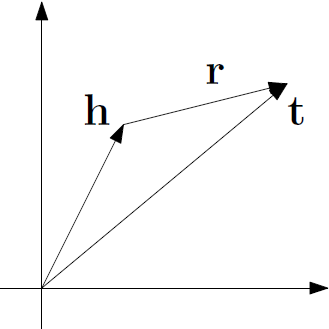
\includegraphics[width=.4\textwidth]{fig/embeddings/TransE.png}
    \caption{TransE representation in 2D Space}
    \label{fig:emb-transE}
\end{figure}

The basic idea behind this model is that the connecting relation between the two entitiy representations makes it so  $h + r \approx t$ as shown by the figure \ref{fig:emb-transE}, It uses the distance scoring function defined by \ref{eq:transE_scoring} accordingly.

\begin{equation}
    \label{eq:transE_scoring}
    f (h, t) = ||h + r - t||_1
\end{equation}
    
TransE is the earliest translation-based embedding model, and it has difficulty dealing with multirelational graphs; it is limited by its simple translation operation as well as its lack of a discrimination policy for all kinds of relations.

Improving on TransE, TransH introduces the concept of hyperplanes translations, in order to overcome the problems of TransE in modeling reflexive multiorigin or multidestination relations (one-to-many, many-to-one, many-to-many)this model enables an entity to have distributed representations when involved in different relations. 

\begin{figure}[!htp]
    \centering
    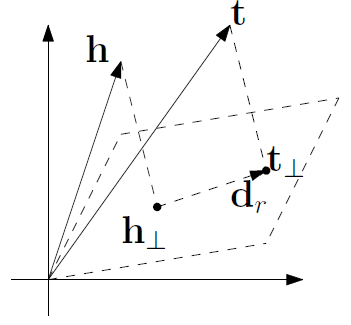
\includegraphics[width=.4\textwidth]{fig/embeddings/TransH.png}
    \caption{TransH representation in 2D Space}
    \label{fig:emb-transH}
\end{figure}

As illustrated in Figure \ref{fig:emb-transH}, the relation translation vector $d_r$ is contained within the plane rather than being connected directly such as in TransE.

for a triple (h, r, t), the embedding h and t are first projected to the plane ($h\bot$, $t\bot$). They are then connected by a translation vector $d_r$ in the hyperplane. The scoring funtion is described as by \ref{eq:transH_scoring}

\begin{equation}
    \label{eq:transH_scoring}
    f (h, t) = || (h - w^\tau_r |hw_r) + d_r - (t-w^\tau_r tw_r) ||^2_2
\end{equation}
\begin{center}
    $w_r, d_r \in \mathbb{R}$
\end{center}

Improving on then TransH model appears TransR\cite{} which innovates by using a relation-specific space to handle different relations. As an entity may have multiple semantical interpretations different relations focus on different ones. TransR models entities and relations in distinct spaces, entity and relation spaces and performs translation in the corresponding relation space.

\begin{figure}[!htp]
    \centering
    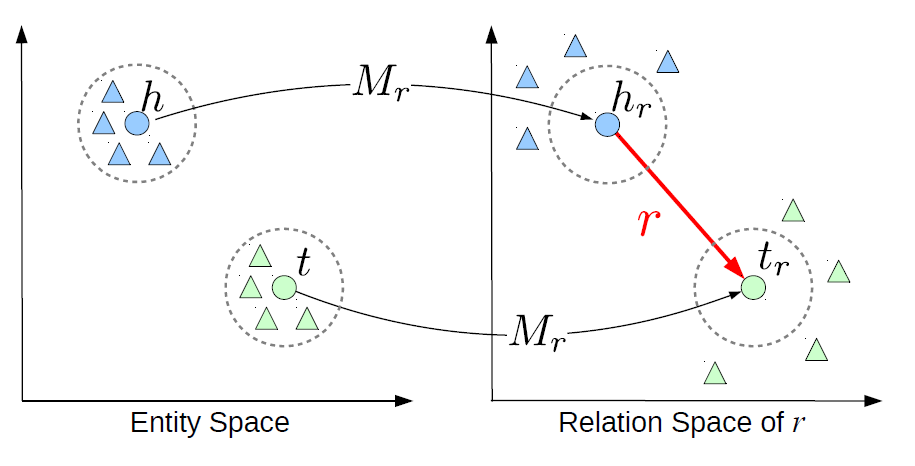
\includegraphics[width=.7\textwidth]{fig/embeddings/TransR.png}
    \caption{TransR representation in 2D Space}
    \label{fig:emb-transR}
\end{figure}

Figure \ref{fig:emb-transR} shows a simple rendition for the TransR model, it depicts how for a given triple (h, r, t), entities ``h'' and ``t'' are projected into the relation space for relation ``r'', then a translation is performed in said vectorial space. This relation specific space also shows how other entities appear further away from the source triple as they are not close semantically for that particular relation space. TransR scoring function \ref{eq:transR_scoring} is very closely related to TransE scoring function with the key difference that is performed in a diferent space.

\begin{equation}
    \label{eq:transR_scoring}
    f(h, t) = ||h_r + r - t_r||^2_2
\end{equation}

Several iterations of the Trans(+letter) model have been proposed as improvements to these previously mentioned approaches, all of them iterating on the idea of decoupling entity and relations interactions to then perform a translation operation of some sort.

To conclude this section RotatE\cite{} presents an improvement from previous techniques by defining each relation as a rotation from the ``h'' to ``t'' in a complex plane and the same vector space as shown in figure \ref{fig:emb-rotatE}.

\begin{figure}[!htp]
    \centering
    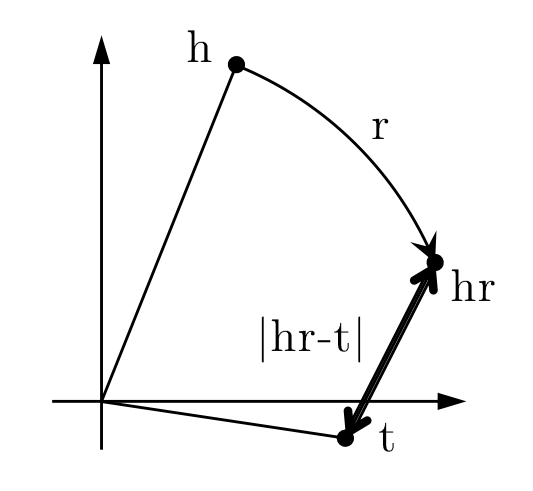
\includegraphics[width=.4\textwidth]{fig/embeddings/RotatE.png}
    \caption{RotatE in a 2D plane}
    \label{fig:emb-rotatE}
\end{figure}

RotatE maps the head and tail entities ``h'' and ``t'' to complex embeddings then, it defines a mapping function induced by each relation ``r'' as an rotation from ``h'' to ``t'' where $t = h \circ r, where |r_i| = 1$ and $\circ$ is the Hadmard product.
By defining each relation as a rotation in the complex vector spaces, RotatE can model and infer relation patterns such as symmetry/antisymmetry, inversion and composition. 

\begin{equation}
    \label{eq:rotatE_scoring}
    f(h, t) = ||h \circ r - t||
\end{equation}

The distance function of RotatE \ref{eq:rotatE_scoring} corresponds to a counterclockwise rotation by $\theta_r,i$ radians about the origin of the complex plane, and only affects the phases of the entity embeddings in the complex vector space.


\section{Semantic information models}\label{sec:emb-semantic}
Semantic information-based models usually use similarity-based functions to define scoring functions for traditional semantic-matching models or introduce additional information to mine more knowledge for recently proposed models.

Traditional models match the latent semantics of entities and relation embeddings to measure the plausibility of a triple, however, these models suffer from high computational complexity.

More recent models fuse various additional information to obtain better performance to mine deeper semantic informationat the bottoms of graphs. The additional information includes path information, order information, concepts, entity attributes, entity types and so on.

Word2vec\cite{} goal is learning high-quality word vectors from huge data sets with billions of words, and with millions of words in the vocabulary by using distributed representations of words learned by neural networks following stochastic gradient descent methods and backpropagation.

\begin{figure}[!htp]
    \centering
    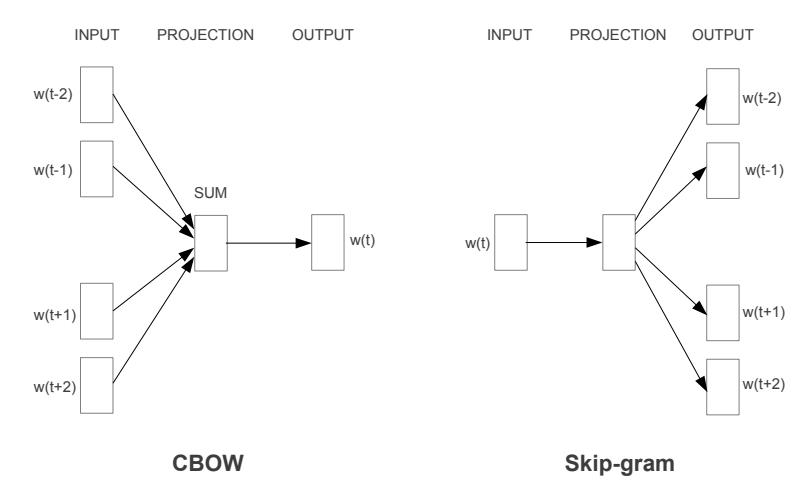
\includegraphics[width=.75\textwidth]{fig/embeddings/Word2Vec.png}
    \caption{Word2Vec models}
    \label{fig:emb-rotatE}
\end{figure}

It consist of two methods, a continuos bag-of-words model and a skip-gram model. The first of the two closely resembles a feedforward NNLM (Neural Network Language Model), where the projection intermediate layer is altered by all words in the input, therefore, all words alter the composition of the NN and their vectors are averaged.

The second model tries to maximize the classification of a word based on the sentence it is contained within. the entire context sentece is fed into a log-linear classifier which tries predict words before and after the current word.

\todo{inser GlovE here.}
GlovE \cite{} appears 

\section{Tensor Factorization models}\label{sec:emb-tensor}
Tensor factorization try to solve KG completion tasks by relying on the fact that a Knowledge Graph can be represented as tensors where the relational data can be represented as a {0, 1}-valued third-order tensor Y, and, if a relation (h, r, t) is true it meets $Y_{h,r,t} = 1$, KGC can be framed as a 3rd-order binary tensor completion problem.

The first apporach to take advantage of the tensors being able to represent a Knowledge Graph was RESCAL \cite{}, which takes the inherent structure of relational data into account by operating over this tensor representation of.

\begin{figure}[!htp]
    \centering
    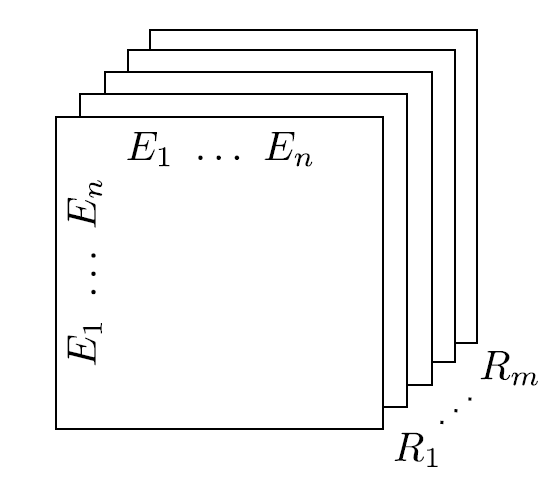
\includegraphics[width=.45\textwidth]{fig/embeddings/Rescal.png}
    \caption{Tensor representation of a Knowledge Graph with entities $E_1,...,E_n$ and relation $R_1,...,R_n$}
    \label{fig:emb-rescal}
\end{figure}

RESCAL applies a decomposition into directional components approach which is capable of detecting correlations between multiple interconnected nodes. It decomposes them into a 3-way tensor as shown in figure \ref{fig:emb-rescal}, two dimensions are generated by the concatenated entity vectors and the third represents the relations matrix.
In RESCAL, entities are expressed as vectors $v \in \mathbb{R}^d$ and relations are expressed as matrices $M \in \mathbb{R}^{d \times d}$  to calculate the score of a fact (h, r, t) a bilinear function is applied as defined by equation \ref{eq:rescal_scoring}.

\begin{equation}
    \label{eq:rescal_scoring}
    s(h, r, t) = v^T_h M_r v_t
\end{equation}

where $vh, vt \in \mathbb{R}^d$ are entity embeddings, and $M_r \in \mathbb{R}^{d\times d}$ is the matrix associated with the relations between them.

Continuing the work on tensor factorization we find DistMult \cite{}, an approach that tries to learn representations for entities and relations via a neural network in which the first layer projects a pair of input entities to low dimensional vectors, and the second layer combines them into a the input of the bilinear scoring function \ref{eq:distmult_scoring} which represents the relation between them looking to maximize this score.

\begin{equation}
    \label{eq:distmult_scoring}
    g^b_r (e1, e2) = e_1^T W_r e_2
\end{equation}

where $e_1$ and $e_2$ are the learned entity vectors and $W_r$ is the tensor operator. 

Furthering this line of work is complEx \cite{}, as suggested by the name instead of using embeddings containing real numbers it furthers the idea of complex embeddings, similarly to rotatE as seen previously. ComplEx argues that the standard dot product between embeddings can be a very effective composition function when using complex vectors.

This instance of the dot product involves the conjugate-transpose of one of the two vectors. As a consequence, the dot product is not symmetric any more, and facts about antisymmetric relations can receive different scores depending on the ordering of the entities involved.

Thus complex vectors can effectively capture antisymmetric relations while retaining the efficiency benefits of the dot product, that is linearity in both space and time complexity.

A key difference with the RotatE model which also focuses on these complex spaces is that ComplEx applies a tensor factorization approach in a bilinear way, this means that the same entity will have two different embedding vectors, depending on whether it appears as the subject or the object of a relation.

Finally the TuckER \cite{} model named after the author of Tucker decomposition \cite{} applies the principles of said technique to the tensor factorization model, by decomposing a tensor into a core tensor multiplied by a matrix along each mode as shown in figure \ref{fig:emb-tucker}, TuckER generalizes the problem presented in previous approaches.

\begin{figure}[!ht]
    \centering
    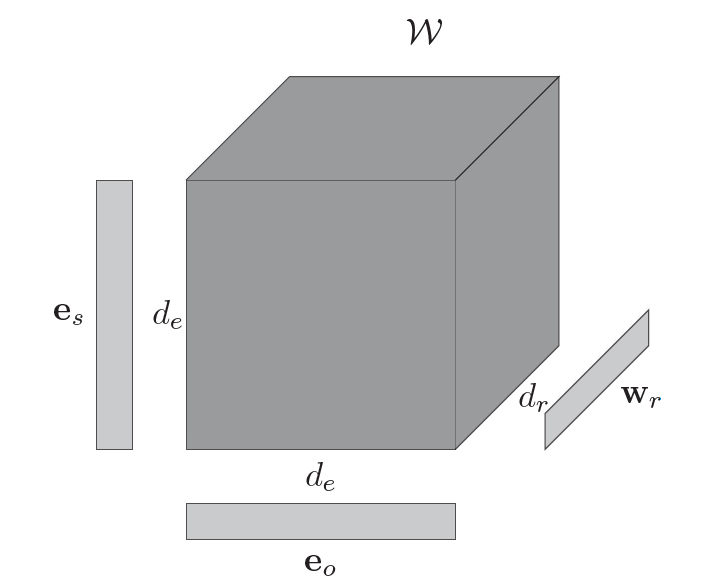
\includegraphics[width=.45\textwidth]{fig/embeddings/TuckER.png}
    \caption{TuckER architecture}
    \label{fig:emb-tucker}
\end{figure}

Using the Tucker decomposition for link prediction on the tensor representation of a knowledge graph, with entity embedding matrix $\mathcal{E}$ relation embedding matrix $\mathcal{R}$ the scoring function for this model is as shown in figure \ref{eq:tucker_scoring}

\begin{equation}
    \label{eq:tucker_scoring}
    \theta (h, r, t) = \mathbb{W} x_1 h x_2 w_r x_3 t
\end{equation}

where h, t are the rows of matrix $\mathcal{E}$ representing the subject and object entities vectors, $w_r$ the rows of the relation matrix and $\mathbb{W}$ is the core tensor to predict.

\section{Neural network-based models}\label{sec:emb-nn}

Neural networks can intelligently capture the semantic features of entities and relations and reasonably model the semantic relationships between discrete entities, which can help learn more accurate embeddings in the context of Knowledge Graphs problems. 

The improvement of Deep Neural Networks (DNNs), Recursive Neural Network (RNNs) or Graph Neural Networks(GNNs) along the previously discussed techniques made it an obvious path for research where NN models were tailored to generating this embedding representations of KG components. However NN models apply non-linear transformations to the data they are provided in which they lose explainability in the generative process.

One of the initial approaches for this method is Neural Tensor Networks (NTN) \cite{} it is a link prediction method which replaces a standard linear neural network layer with a bilinear tensor layer that directly relates two entity vectors across multiple dimensions making it so entities are represented as an average of their constituting word vectors. The model computes a score of how likely it is that two entities are in a certain relationship by the following NTN-based function shown in figure \ref{fig:emb-ntn}

\begin{figure}[!ht]
    \centering
    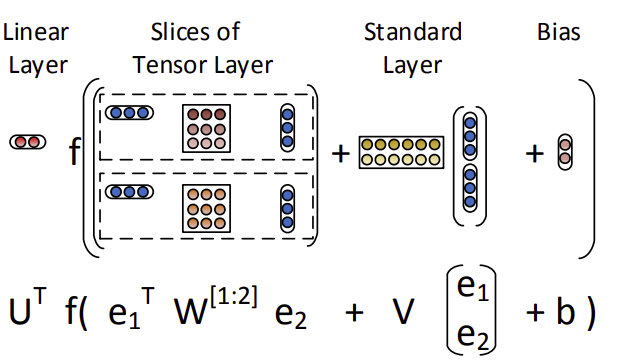
\includegraphics[width=.65\textwidth]{fig/embeddings/NTN.png}
    \caption{NTN layer}
    \label{fig:emb-ntn}
\end{figure}

ConvE \cite{} iterates upon the idea presented by NTN by using a multi-layer convolutional network model in order to be more parameter efficient than its predecessors and competitors such as DistMult. 

ConvE utilizes 2D convolutions over embeddings to predict missing links in knowledge graphs. It is the simplest multi-layer convolutional architecture for link  prediction. It is defined by a single convolution layer, a projection layer to the embedding dimension, and an inner product layer.

using a 2-dimensional convolution layer increases the expresiveness of the model as it increases the number of interaction points, thus being able to extract more feature interactions between two entity embeddings.

InteractE \cite{} improves upon ConvE by providing three key ideas feature permutation, a novel ``checkered'' feature reshaping, and circular convolution as the expressiveness of a model can be enhanced by increasing the possible interactions between embeddings.

\begin{figure}[!ht]
    \centering
    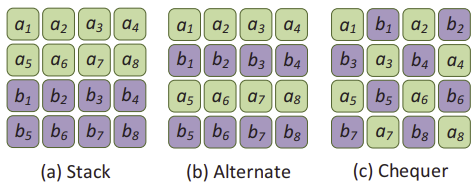
\includegraphics[width=.65\textwidth]{fig/embeddings/InteractE.png}
    \caption{InteractE checkered patter for tensor reshaping.}
    \label{fig:emb-interactE}
\end{figure}

\textit{Feature Permutation}: Instead of a fixed order for inputs InteractE allows for a mutable input order increasing the interaction between entity embeddings by allowing permutation between these inputs. However, the number of distinct interactions across all possible permutations is very large. So, for t different permutations, we can expect the total number of interactions to be approximately t times the number of interactions for one permutation.

\textit{Checkered Reshaping}: applies a reshape function for tensors that intertwines the features as seen in figure \ref{fig:emb-interactE}, which captures maximum heterogeneous interactions between entity and relation features.

\begin{figure}[!ht]
    \centering
    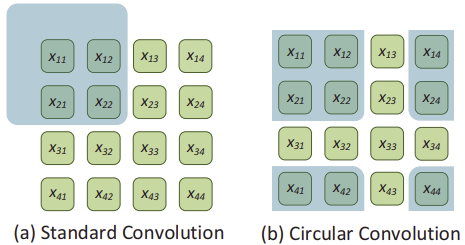
\includegraphics[width=.65\textwidth]{fig/embeddings/interactE_convolutions.png}
    \caption{InteractE circular convolution.}
    \label{fig:emb-interactE_conv}
\end{figure}

\textit{Circular Convolution}: Ciruclar convolution allows for a wraparound of the features selected for the convolution operation, as shown in figure \ref{fig:emb-interactE_conv}.

Also improving on ConvE we have ParamE, which makes use of translational properties such as the models in section \ref{sec:emb-translations} and neural networks non linear fitting skills such as previous models from this section.

\begin{figure}[!ht]
    \centering
    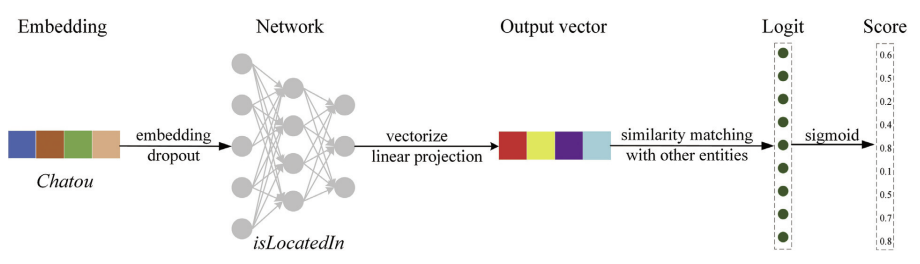
\includegraphics[width=\textwidth]{fig/embeddings/ParamE.png}
    \caption{ParamE model overview.}
    \label{fig:emb-paramE}
\end{figure}

In ParamE, head entity, relation, and tail entity embeddings are the input and output of a neural network respectively. taking neural network parameters as relation embeddings makes ParamE much more expressive and translational. entity and relation embeddings in ParamE belong to from feature space and parameter space respectively, which keeps them mapped into two different spaces. The main idea of ParamE is to regard NN parameters as relation embeddings, which makes it  expresive and translational.

ParamE is a general architecture for 3 separate NN models multilayer perceptrons,convolution layers, and gate structure layers, in which the latter is shown to outperform the other two measures.

Finally MEI \cite{} multi-partition embedding interaction model introduces the division of embeddings into multiple partitions, restricting the interactions in a triple to only entries in the corresponding embedding partitions of (h,r,t).

\begin{figure}[!ht]
    \centering
    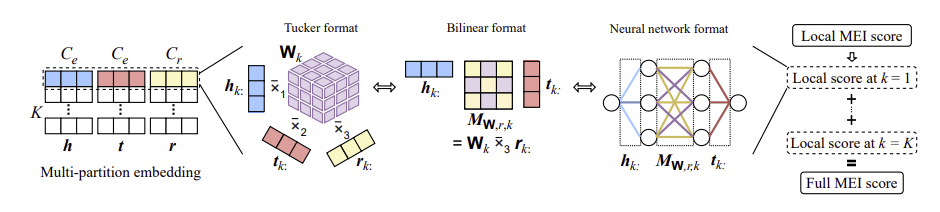
\includegraphics[width=\textwidth]{fig/embeddings/MEI.png}
    \caption{MEI model}
    \label{fig:emb-MEI}
\end{figure}

Interactions in each partition is done using the tucker format\cite{} to learn general linear interaction mechanisms figure \ref{fig:emb-MEI}. The total score for the model is the sum of all local interactions. 

In each triple (h, t, r), the entities and relations embedding vectors $h, t \in \mathbb{E}^{D_e}$ , and $r \in mathbb{R}^{D_r}$ are divided into multiple partitions, the score function of MEI \ref{eq:MEI_scoring} is defined as the sum score of $\mathcal{K}$ local interactions, with each local interaction being modeled by the Tucker format.

\begin{equation}
    \label{eq:MEI_scoring}
    \mathcal{S}(h, r, t; \theta) = \mathbb{W}_k x_1 h_k x_2 t_k x_3 r_k
\end{equation}

\section{Summary}\label{sec:emb-summary}
% In this chapter, we have presented an overview of the existing methods for Knowledge Graph completion in the literature that rely on latent triple representations. We have introduced and described the models that use tensors to model a KG, and then factorize those tensors to obtain a predictive model. We have also presented the models that embed entities in a higher-order space and perform translations on them to find missing knowledge. Finally, we have enumerated the methods that use neural networks to perform Knowledge Graph completion, and we have presented the neural network architectures that are commonly used for this task.

brief summary of all the facts presented.
    \chapter{Reinforcement Learning}\label{chap:reinforcement}

\chapterQuote{
    \textit{``Caminante, no hay camino, se hace camino al andar.''}\\
    \textit{(``Traveler, there is no path, you make your path as you walk.'')}
    }{--- Antonio Machado}

\chapterAbstract{A}{qui hablamos tanto del RL de base y su historia y como funciona hasta de como se plaica en los grafos de conocimiento y porque provee de un razonamiento intrinseco.

Mencionamos tambien metodologia de los diferentes algoritmos como PPO, SAC, reinforce vs Actor critic etc etc...}

\section{Introduction}\label{sec:rl-intro}
An explanation of how reinforcement learning works and where its usefull.
% A relational path is a sequence of relations that connect two entities together in a Knowledge Graph. There can be many such paths between any two entities, and they can vary in length and complexity. Given that these paths can provide an interesting insight on how related two entities are, many researchers have developed methods to analyze them to learn what constitutes correct knowledge. 

% Generally, these methods generate features that characterize the information contained in each path, and then train classifiers to predict the existence of missing relations based on these features. Due to the high number of possible paths that can exist between two entities, such methods usually use techniques like random walks to restrict the amount of paths that are analyzed, possibly constraining their effectiveness.

% To solve this issue, other methods analyze graph neighborhoods, which refer to the entities and relationships that are directly connected to a given entity in a Knowledge Graph. This allows KG completion method to focus on a much more reduced amount of information that is more likely to accurately characterize an entity.

% In this chapter, we present an overview on the methods that rely on these techniques to complete a Knowledge Graph. We first introduce the methods that rely purely on relational paths and their characterization. Next, we present the methods that analyze entity neighborhoods. Finally, we discuss more advanced methods that combine these approaches with techniques from the previous chapter.

\section{Algorithms}\label{sec:rl-algorithms}
We categorize and evaluate the different algorithms and progress that has been made in the field of reinforcement learning 

% A relational path is simply a concatenation of triples that connect an entity to some other entity through a number of relations. Naturally, any Knowledge Graph has an abundance of possible paths to, from, or between entities. The idea of analyzing such paths to learn what constitutes valid knowledge has led to many research works.

% One of the first approaches that exploited relational paths in a Knowledge Graph was the Path Ranking Algorithm (PRA), proposed by \citet{lao2011}. PRA uses random walks to generate a set of paths between a given pair of entities in a depth-first manner. The generated paths are then transformed into a series of features that aim to characterize the information contained in it. These features are ultimately used to train a binary log-linear classifier, which learns whether a direct relationship should exist between two entities according to the paths that are already present between them. However, PRA is not without limitations. The number of possible paths between a pair of entity can be very high, limiting its scalability. Additionally, the randomly guided paths that it uses may miss information just by mere chance.

% Aiming to improve PRA, \citet{gardner2015} introduced the Subgraph Feature Extraction (SFE) method. In opposition to PRA, SFE uses a breadth-first search that is not randomly guided, in order to better characterize the portion of the KG between two entities. SFE also requires the creation of a handmade ``Alias'' relation, which relates entities in the same KG that refer to the same element in the real world. It is able to achieve more expressive results than PRA, making it easier for the human user to understand what constitutes a good path that may be indicative of the existence of a direct relation between two entities.

% \citet{gardner2013} also proposed an extension of PRA that addresses the issue of potentially having to consider a very high number of paths. It considers the semantic similarities between the relations of a Knowledge Graph, and uses them to merge very similar paths together, greatly reducing the number of paths that need to be analyzed afterwards. This addition increases the effectivity of PRA in the NELL Knowledge Graph, although the authors do not provide data for any other KGs.

% \citet{nastase2019} proposed the Abstract Path Model (APM), which produces an abstract graph from a KG, and then focuses on extracting relevant abstract paths from it. These abstract graphs provide a more general representation of the high-level relations between entities, and thus the paths that can be traced in it represent more high-level knowledge. Additionally, this abstract representation is, as a general rule, considerably smaller than the KG it is derived from and not very computationally taxing to obtain, which aids in its application to larger graphs.

% \citet{gu2015} introduced the Trans-COMP method, which proposes a different strategy. Rather than analyzing a large number of paths between two entities to try to characterize the pair, it only uses a single path. Precisely, it aims to select the path that provides the highest predictive capabilities of the existence of a given relation. \citet{toutanova2016} further refine this idea with their All-Paths method by providing an explicit way to represent the intermediate entities that can be found in such a path and, additionally, enabling the method to consider more paths.

% A number of other authors have also researched alternative ways to select and learn from the best paths in a Knowledge Graph. \citet{jiang2017} proposed the APCM model, which assigns different weights to the found paths and combines them based on these weights. Furthermore, the PRCTA model introduced by \citet{lei2019} employs an attention mechanism \cite{vaswani2017} to construct and select the paths, which allows it to work satisfactorily in more sparse KGs.

\section{RL in KGs}\label{sec:rl-RLinKGs}
an overview of all approaches that appeared in the field. tables and all.
% The previous chapter introduced the main ideas behind how embeddings and neural networks can be applied to Knowledge Graph completion. Some authors have proposed a series of approaches that combine path-based information with these techniques, in order to guide the path finding process towards the most significant path, avoiding having to explore a very large number of them.

% An example of this is the PATH-RNN technique, which was proposed by \citet{neelakantan2015}. In addition to using path-based information, PATH-RNN uses the embedded representations of the relations in a path to further characterize it. It uses a recursive neural network (RNN) to combine these embeddings together, resulting in a single embedding that contains information about the entire path. For this reason, it can operate using paths of any length. Additionally, due to the fact that it operates on the embedded representations of the relations, which in turn capture semantic meanings, it can in theory predict relations that were not present in the KG at the time of training the model. Figure~\ref{fig:path-rnn} graphically illustrates this idea.

% \begin{figure}[!htp]
%     \centering
%     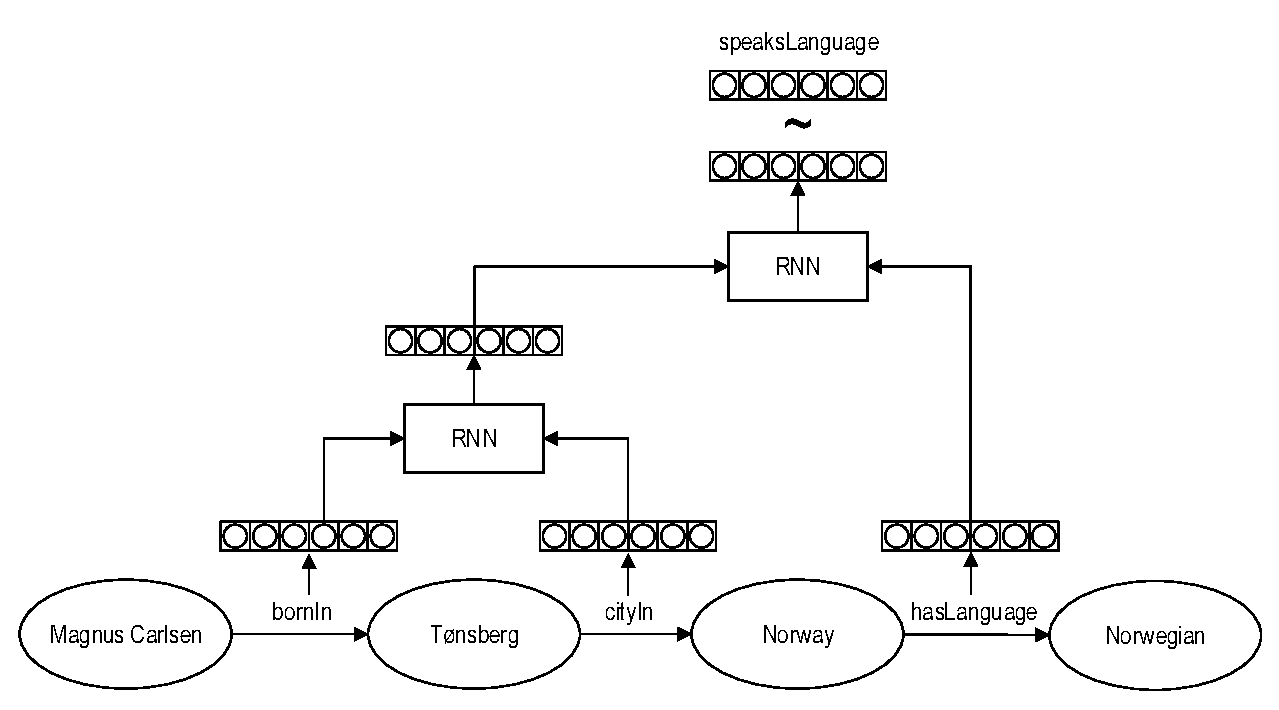
\includegraphics[width=\textwidth]{fig/paths/pathrnn}
%     \caption{Overview of the PATH-RNN method}
%     \label{fig:path-rnn}
% \end{figure}

% \citet{das2017} improve the previously discussed PATH-RNN method with their Single-Model proposal. They point out that taking the embeddings of the entities in a path into account can provide useful information. To represent a path, they recursively combine the embeddings of both the entities and relations in it using RNNs. Furthermore, they propose using a number of different functions to select the best path: \textit{Top-K}, \textit{Average} and \textit{LogSumExp}. They experimentally conclude that the \textit{LogSumExp} function performs better when completing a Knowledge Graph. Figure~\ref{fig:path-single} displays a visual overview of Single-Model. In this Figure, entity embeddings are represented in blue, and relation embeddings in orange. The path that is being considered is the same as in Figure~\ref{fig:path-rnn}.

% \begin{figure}[!htp]
%     \centering
%     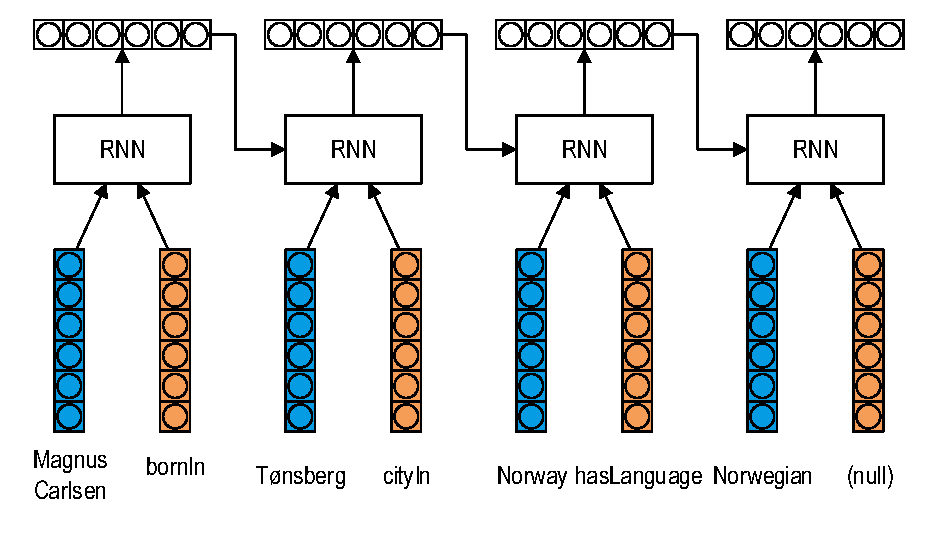
\includegraphics[width=.9\textwidth]{fig/paths/singlemodel}
%     \caption{Overview of the Single-Model method}
%     \label{fig:path-single}
% \end{figure}

% \citet{xiong2018} proposed GMatching, a technique that specializes in extracting information from KG neighborhoods using relatively infrequent relations, which are traditionally considered more challenging due to the reduced amount of information about them present in the graph. GMatching is comprised of two main components: a neighbor encoder, which creates an embedded representation for an entity in a neighborhood; and a matching checker, which computes the similarity of two entity embeddings created by the first component. A visual representation of this proposal is provided in Figure~\ref{fig:path-gmatching}. The meaning of the colors is the same as in the previous Figure.

% \begin{figure}[!htp]
%     \centering
    
%     \subfigure[An example KG]{
%         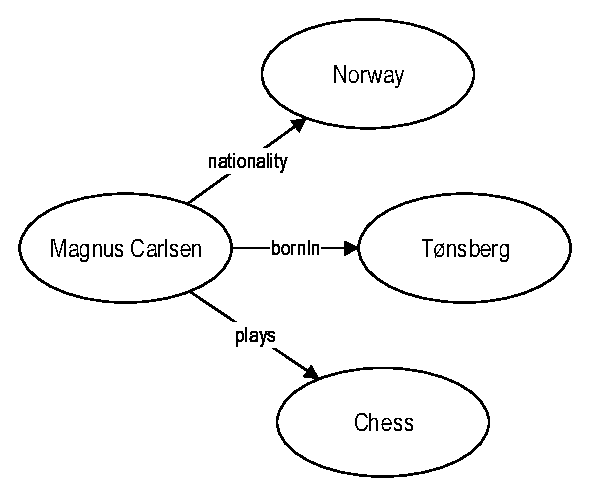
\includegraphics[width=.45\textwidth]{fig/paths/gmatching-a}
%     }\\
%     \subfigure[Encoding of the neighborhood of the entity \textit{Magnus Carlsen}]{
%         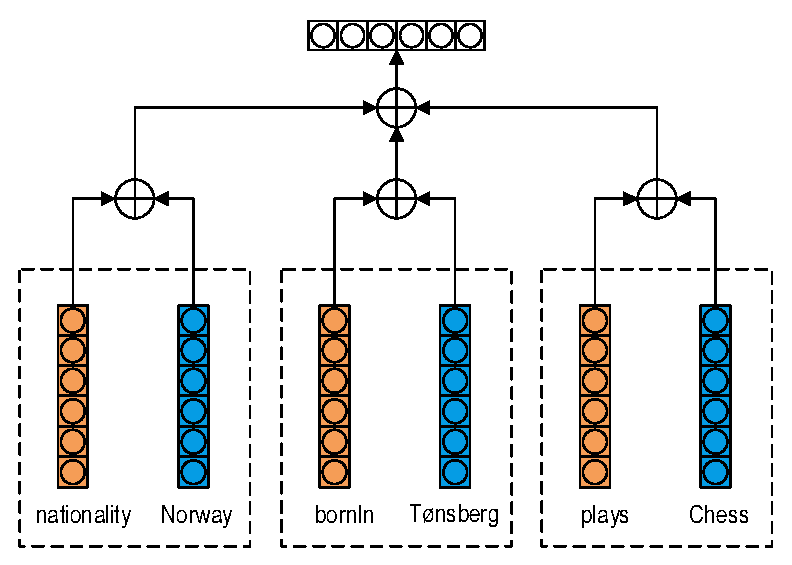
\includegraphics[width=.7\textwidth]{fig/paths/gmatching-b}
%     }

%     \caption{Overview of the GMatching method}
%     \label{fig:path-gmatching}
% \end{figure}

% \citet{shen2017} proposed Implicit ReasoNets (IRNs), a neural network architecture that is able to reason about paths of different lengths in a KG. It is an encoder-decoder model that is governed by a central controller, which allows the whole process to be carried out with no human intervention. Also, it introduces the usage of a shared memory that implicitly stores relevant information about the graph, allowing it to be more efficient and have a smaller memory footprint.

% Additionally, a number of improvements have been made to the baseline translational models to help them leverage path information in several ways. For instance, \citet{lin2015} have proposed PTransE, an extension of TransE that uses path information in its confidence function. Its goal is to give a higher confidence score to those entities that are well-connected together by means of paths that are semantically similar to the relation in the triple that is being evaluated.

% \citet{garcia-duran2015b} proposed RTransE, which represents paths as a series of translations in the embedded space defined by the TransE model. For efficiency reasons, RTransE is limited to using only paths that contain two relations. Likewise, \citet{xiong2018b} introduced PTransD, an enhancement of TransD that performs subsequent translations to model paths. However, PTransD uses two embeddings to represent each entity, to perform operations in parallel.

\section{Explainability?}\label{sec:rl<REPLACE THIS>}
this needs some more classification I`m not sure how yet, maybe when I begin writing it...

% Considering the possible paths between two entities is undoubtedly helpful, but this concept can be expanded further. Rather than a single path, we can consider the entirety of the region of a Knowledge Graph around a certain entity, in other words, its neighborhood. The concept of entity neighborhood is visually shown in Figure~\ref{fig:path-neighborhood}, which depicts the closest and more extended neighborhoods of an entity shown in the center.

% \begin{figure}[!htp]
%     \centering
%     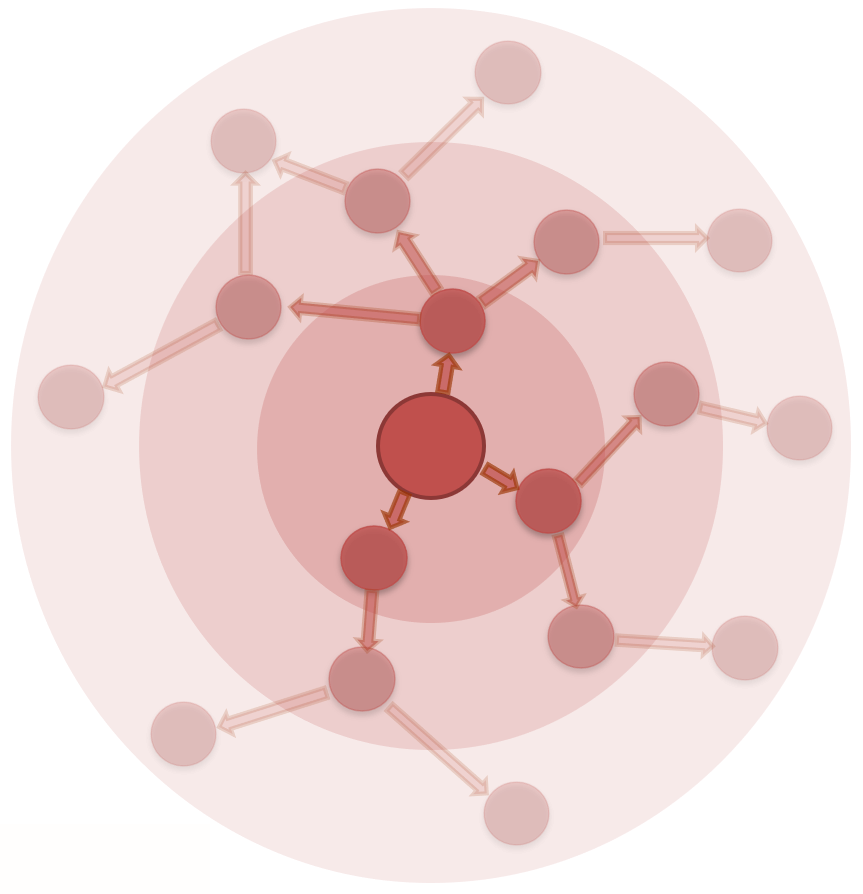
\includegraphics[width=.7\textwidth]{fig/paths/neighborhoods-b.png}
%     \caption{A visual representation of entity neighborhoods}
%     \label{fig:path-neighborhood}
% \end{figure}


% Given a pair of entities, their neighborhoods can be analyzed to determine if a relation should be present between them. This idea has been put to practice by a number of authors.

% \citet{bansal2019a2n} proposed the A2N method, which aggregates the entities in a neighborhood together to obtain a more compact representation of said neighborhood. It uses an attention-based mechanism to focus on the most prominent entities, giving a trustworthy representation of the entities surrounding another one. Additionally, it is designed such that the computational cost of the method does not increase greatly with the size of the neighborhoods.

% The use of attention-based mechanisms in this regard has not gone unnoticed by other authors. \citet{wang2019} have proposed LAN, another approach that aggregates the contents of an entity neighborhood together, however, the attention-based technique that they propose uses weights to give more importance to more relevant entities. \citet{kong2019} also proposes using attention to filter out possibly irrelevant relations in the graph, allowing the models to focus only on more meaningful information, which is especially relevant in the case of heterogeneous Knowledge Graphs. Similarly, \citet{nathani2019} introduced the KBAT method, which is able to capture information from both the entities and the relations in a KG neighborhood. 

% \citet{zhang2020} further the previous idea by adding a weighted attention system to both entities and relations, acknowledging that not all knowledge in the KG is equally useful. Two different attention-based mechanisms are used in their proposal. First, the relation-level attention provides an intuition for which connections from an entity may provide more useful information. Then, the reached entities are considered according to their entity-level attention. This composite, hierarchical attention mechanism allows it to outperform other attention-based proposals.

% \citet{ferre2019} proposes finding missing information by finding similar entities in commonly occurring graph patterns, through the application of concepts of nearest neighbors \cite{denoeux1995}. It does not require any sort of pre-processing of the Knowledge Graph, making it very efficient. Furthermore, its reliance on graph patterns makes it a more interpretable method than other similar proposals.



\section{Summary}\label{sec:path-summary}
The contents of this chapter have provided an overview of the methods to perform Knowledge Graph completion that use relational paths. We have first listed the most prominent scientific proposals that extract paths from a KG and characterize them using features, to learn which paths can be predictive of correct knowledge. Afterwards, we have centered on the proposals that use entity neighborhood information in a number of ways. Finally, we have introduced the approaches that merge together path-based information with latent entity representations, entity and relation embeddings, and neural networks.
    % removed due to time constraints, will include it later, if time allows for it.
    % \chapter{Completion and Reasoning in literature}\label{chap:other_approaches}

\chapterQuote{\textit{``Logic, like whiskey, loses its beneficial effect when taken in too large quantities.''}}{--- Edward J. M. D. Plunkett, Lord Dunsany}

\chapterAbstract{S}{Context for completion and reasoning in detail from the papers...}
% ogical rules are commonly used to perform Knowledge Graph completion. The proposals that employ these kinds of rules usually mine them first using the triples present in the graph, to generalize specific knowledge stored in it. Then, the extracted rules are used to materialize knowledge in the form of new triples, which can be added back to the KG. In this chapter, we provide an overview of the various ways in which this has been carried out by previous works. It is organized as follows: Section~\ref{sec:rule-intro} lays out the foundational concepts, Section~\ref{sec:rule-ilp} presents the existing methods for mining logical rules from a Knowledge Graph, Section~\ref{sec:rule-cands} introduces the proposals that aim to reduce a set of possible candidate triple using rules, Section~\ref{sec:rule-hybrid} enumerates the approaches that combine rules with other popular ways to complete KGs, and Section~\ref{sec:rule-summary} concludes the chapter.

%LO QUE DANI DICE AQUI ES MUY INTERESANTE.
% Obviamente aquí no se discuten en profundidad los otros métodos, pero no hablaría de candidate mining, sino de:

% 1) Rule mining, que intentan buscar algún patrón que se correlacione con la aparición de las relaciones (por ejemplo, tener parte del contexto común, la presencia de alguna otra relación etc.) Puedes mencionar que su ventaja es que no requieren el uso de embeddings, por lo que son aplicables fácilmente a nodos nuevos, y además ofrecen un completado con explicación. La desventaja es que las reglas pueden estar basadas en calculos más costosos (por ejemplo el solapamiento del contexto de dos nodos, como hace CAFE) si se quieren aplicar a toooodos los posibles hechos de un grafo, aunque entonces se puede aplicar una técnica simplificada que de forma rápida haga una primera criba (candidate filtering).

% 2) Neural-embeddings based, que usan los embeddings de redes neuronales mencionados en la sección anterior para evaluar las posibles tripletas, normalmente o aplicando una red neuronal a los embeddings, o realizando una simple operación con los embeddings y comprobando si el valor resultante es alto o bajo. Por ejemplo TransE coge el embedding de la entidad 1, le suma el de la relación, y mira si el resultado es cercano al embedding de la relación 2. Son rápidas de aplicar pero requiere el entrenamiento de todos los embeddings cada vez que se actualiza el grafo. Además no son explicables.

% 3) Los métodos basados en reinforcement learning, que se parecen a la primera categoría en tanto que la predicción es explicable y basada en la presencia de ciertas relaciones, y a la segunda en tanto que se usan los embeddings de nodos y relaciones

% Entiendo que la mayoría de lo que decir de las dos primeras categorías es básicamente cosas que puso Agustín. Para lo tercero ya lo que hace es introducir un poco lo que se detallará en la siguiente sección.


please ignore the Sections...

\section{Introduction}\label{sec:rule-intro}
% Knowledge Graphs are essentially large and incomplete collections of facts about a certain domain. One possible way to complete them is to observe which facts occur frequently together, and then express this relationship as a rule for those combinations that are observed very often. For example, if a person was born, studied and died in a city, it is very likely that they hold the nationality of the country in which that city is located. More formally, this can be expressed through the following logical rule, where $p$ is a person, $c$ is a city, and $C$ is a country:

% \[
% bornIn(p, c) \wedge studiedIn(p, c) \wedge diedIn(p, c) \wedge cityIn(c, C) \rightarrow hasNationality(p, C)
% \]

% These rules are called first-order rules, and they represent explicit knowledge, easy for humans to understand and reason about, in opposition to most latent representation models. They are composed of two elements: the body of the rule (left-hand part) represents the logical condition that must be met, and the head (right-hand part) is the knowledge that is considered to be true if the condition is also true.

% To complete a Knowledge Graph, one can first extract such rules from it, by observing common appearances of these kind of patterns. Then, the rules can be applied to materialize the head of a rule whenever its body exists, generating new explicit knowledge \cite{stepanova2018}. This process is visually depicted in Figure~\ref{fig:rule-process}.

% \begin{figure}[!htp]
%     \centering
%     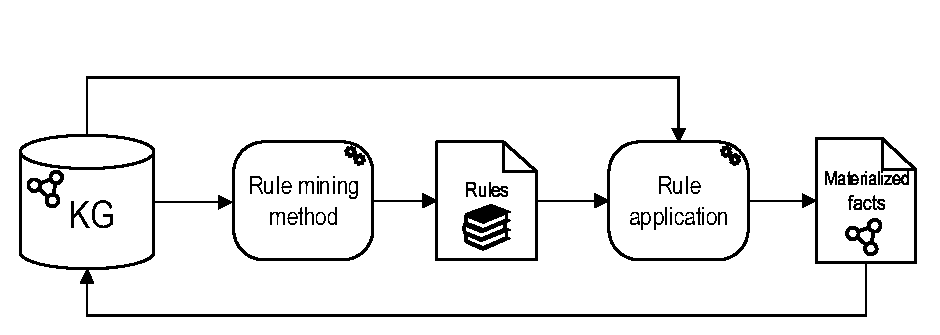
\includegraphics[width=.85\textwidth]{fig/rules/rule_process}
%     \caption{Extracting and applying rules on a Knowledge Graph}
%     \label{fig:rule-process}
% \end{figure}

% In this chapter, we present the existing methods in the literature for obtaining and applying first-order rules to complete a Knowledge Graph. First, we introduce the methods that focus solely on rule extraction. Then, we present some applications of first-order rules to the task of candidate filtering. Finally, we discuss some proposals that combine rules with other ideas presented in previous chapters.

\section{Rule mining methods}\label{sec:rule-ilp}
% There are a number of approaches to mine first-order rules in Knowledge Graphs. One of them is using Inductive Logic Programming (ILP) \cite{muggleton1994}, a classical statistical relational learning method that can be used to extract such rules from a collection of facts.

% In this regard, \citet{jiang2016} have proposed using ILP to perform Knowledge Graph completion on KGs that have a strong time constraint component. Such a KG may contain information on whether a person is the president of a country, whose correctness depends on the time period in which it is interpreted. In this proposal, the most common time periods for an assortment of different facts are inferred through ILP, and then used to assess the correctness of future facts. However, it relies on all facts having time annotations, which may not be commonplace.

% \citet{galarraga2015} proposed the AMIE+ method, which generates similar rules using ILP. AMIE+ addresses the fact that, due to the Open World Assumption (OWA), a fact that is not present in a KG should not be considered false, but instead simply unknown. The OWA thus makes it very challenging to generate truly false examples to assess the overall validity of a rule. The authors use a bespoke confidence measure for their rules, known as the partial completeness assumption confidence. AMIE+ improves the efficiency of its predecessor method AMIE \cite{galarraga2013} and can be applied to larger Knowledge Graphs.

% \citet{wang2015} refine this idea with their RDF2Rules method. Contrary to AMIE+, which is limited to only being able to mine one rule at a time, RDF2Rules speeds up the process by parallelizing rule extraction. It achieves this by detecting and extracting frequent relation cycles of a certain length in a KG, which are essentially loops that contain a given amount of relations. An example of such a loop can be found in Figure~\ref{fig:rule-cycle}. Note that the directionality of the edges in a KG is relevant for the existence of a cycle. Once the most common cycles have been obtained, a number of rules can be extracted from them. This is done by iteratively selecting one relation as the head of the rule and the rest as the body, advancing on the loop, and repeating this process until the entire loop has been traversed.

% \begin{figure}[!htp]
%     \centering
%     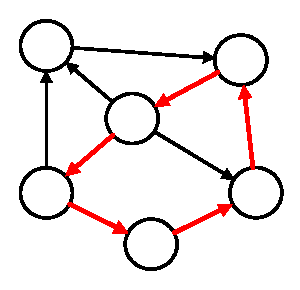
\includegraphics[width=.35\textwidth]{fig/rules/cycle}
%     \caption{A cycle of 5 relations in a sample Knowledge Graph}
%     \label{fig:rule-cycle}
% \end{figure}

% The Never-Ending Language Learning (NELL) system that was proposed by \citet{mitchell2018} also learns knowledge rules from the data that it is constantly provided. These rules are manually screened to ensure a high level of quality, so as to not introduce incorrect facts into a Knowledge Graph. It then applies these rules to generate knowledge that was previously missing.

% Markov Logic Networks (MLNs) \cite{richardson2006} have also been used for the task of completing a Knowledge Graph. MLNs combine the previously discussed rules with probabilistic models, which allows them to derive generalized knowledge from a smaller corpus of facts and to better handle complex and noisy information \cite{yang2017}.

% The use of MLNs for Knowledge Graph completion has been analyzed by \citet{kuzelka2019}. The authors conclude that MLNs can provide a satisfactory performance on this task, assuming that the triples that are missing from the graph are independent from one another and have a roughly equal probability of being true, which is not always the case \cite{borrego2019}.

% \citet{yang2017} presented Neural Logic Programming (NeuralLP), an approach that combines first-order rule mining with sparse matrix multiplication. In this approach, the authors propose using an attention mechanism to further refine the confidence value that is assigned to each individual triple. The main rule mining mechanism in NeuralLP is governed by a central neural controller. Additionally, it is able to learn rules of variable length with more ease than its predecessors.

% Furthermore, \citet{sadeghian2019} introduced DRUM, which extends NeuralLP by analyzing the structure and confidence values of the rules that are being inferred, and then approximating these elements for other rules using tensors. It, however, is only limited to positive examples due to the OWA and is not able to infer negative rules. 

% \citet{rocktaschel2017} proposed NTP, a similar method to NeuralLP, which infers rules by using transitive relations between facts. Their approach requires that such relations be represented as a vector or a tensor, in order to leverage the semantic similarities that are commonly exploited in embedded spaces. It nonetheless suffers from a lesser scalability than the original NeuralLP method, due to the computational complexity that is required to carry out the process of rule inference.

% To address the aforementioned scalability issues, \citet{minervini2018} presented an improved NTP2.0 method. This new version is able to focus only on the most promising rules during the mining process, by using a pooling method that is able to monitor the creation of multiple rules at once.

\section{Candidate filtering}\label{sec:rule-cands}
% Some authors have proposed rule-based techniques for filtering candidate triples, instead of generating new knowledge. The process of generating and applying these rules is fundamentally different: due to the very large number of possible candidate triples, the rules must not be computationally expensive to apply. Additionally, it is not as important for them to be fully correct, since an incorrect fact will be evaluated in more detail further down the KG completion process. It is, however, desirable that the candidate filtering rules exclude as few correct candidates as possible, in order not to hinder the quality of the final set of generated triples.

% \citet{wei2015} proposed the INS method, which uses the previously discussed TransE embedding model to filter out possibly incorrect knowledge. More specifically, they employ TransE to analyze the semantic similarity between the two entities in a triple, and discard the triple if the similarity does not exceed a certain threshold. This results in sets of candidate triples that are smaller than the original ones.

% \citet{shi18} also argued that it is generally not practical to apply any model to the whole set of possible candidate triples, and that it must be narrowed down in some way. In their work, they use a set of simple rules to determine that any given triple $(s, r, t)$ is a valid candidate if another triple with the structure $(\_, r, t)$ is already present in the Knowledge Graph.

% \citet{zhang2019} proposed IterE, an approach that prunes knowledge using graph traversing and random selection. It generates a set of plausible rules and monitors their performance as they are being built, removing those that are found not satisfactory and leaving only a smaller set of rules that can be generated quickly.

% Some of the previously discussed works can also be used for filtering candidate triples. The authors of NTP2.0 \cite{minervini2018} proved that a k-nearest neighbor search can provide satisfactory results to filter out wrong knowledge when inferring rules, which can be performed efficiently.

% Other proposals incorporate parameters that can be fine-tuned to rapidly rule out rules that are not satisfactory. \citet{omran2018} proposed RLvLR, which allows the user to set values for the minimum required confidence for a rule. A similar approach is followed by the already discussed DRUM \cite{sadeghian2019} method.

% Additionally, the AMIE+ method \cite{galarraga2015} can also be used for this purpose. It includes a number of strategies that can be used to prune a set of candidate triples, by producing simpler rules with a high support. Additionally, AMIE+ can perform confidence approximations, which allows it to speed up the rule inference process, making it more appealing for its application to candidate filtering.


\section{Hybrid approaches}\label{sec:rule-hybrid}
% Even though rule-based approaches excel in their explainability, they often have trouble scaling up to very large Knowledge Graphs \cite{shen2022overview}. To overcome this issue, many authors have proposed methods that combine more traditional rule mining with other approaches discussed in previous chapters, to try to guide the rule mining process towards more promising rules.

% One of the first such proposals was made by \citet{wang2015b}, who introduced the r-KGE method. It combines the tensor-based model RESCAL, the embedding-based model TransE, and logical rules. These rules are then used to prune the embedded space using integer linear programming \cite{schrijver1999}, which sees a significant reduction of its size. However, it is not properly equipped to handle N-to-N relations, and its reasoning process can still be quite computationally expensive. The overall model proposed by r-KGE is shown in Figure~\ref{fig:rule-rkge}.

% \begin{figure}[!htp]
%     \centering
%     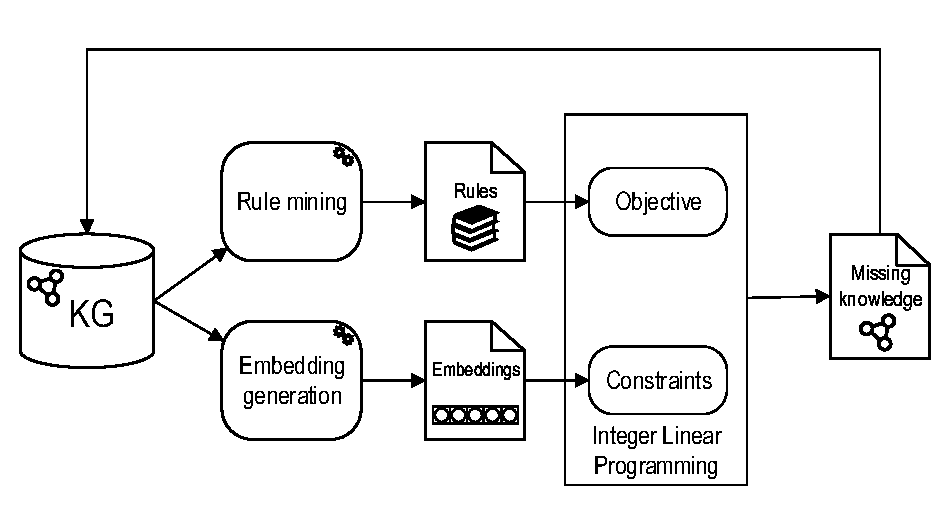
\includegraphics[width=.9\textwidth]{fig/rules/rkge}
%     \caption{Overview of the r-KGE model}
%     \label{fig:rule-rkge}
% \end{figure}

% The previously discussed INS method \cite{wei2015} also incorporates TransE to quickly compute the degree of similarity between entities, and limits the rule reasoning process by taking only the top N most similar entities into consideration. Additionally, this similarity score can provide an approximation of the quality of a rule before it is completely built.

% \citet{guo2016} introduced KALE, another model that combines logical rules and entity embeddings. KALE aims to provide a common ground in which rules and embeddings can directly interact, by representing triples as atomic formulae and rules as combination of these formulae. The semantic similarity information that is intrinsically present in the entity embeddings aids in expanding the predictive capabilities of the rules and their generality. A visual overview of the KALE architecture is provided in Figure~\ref{fig:rule-kale}. In this Figure, entity embeddings are represented in blue, relation embeddings in orange, and scalar confidence values in green.

% \begin{figure}[!htp]
%     \centering
%     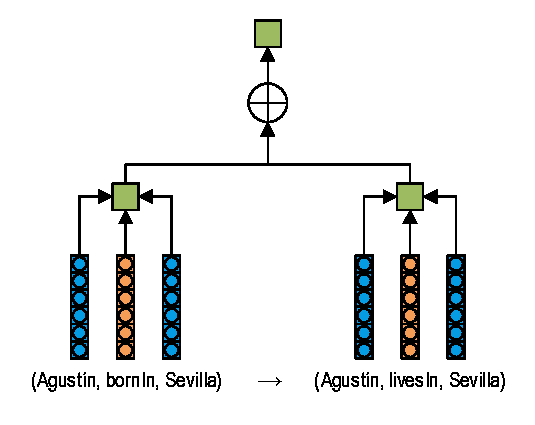
\includegraphics[width=.65\textwidth]{fig/rules/kale}
%     \caption{Overview of the KALE model}
%     \label{fig:rule-kale}
% \end{figure}

% The same authors \cite{guo2018} also presented RUGE, a KG completion technique that combines the same elements in an iterative fashion. Rather than relying on pre-computed entity embeddings, RUGE generates its own embedded space with the aid of logical rules. Additionally, RUGE is able to operate on Knowledge Graphs that has both labeled and unlabeled triples. A series of logical rules are applied on the unlabeled triples to label them. Then, the labeled triples are used to rectify and improve the embedded space so that it better captures the relations between the entities. The improved embedded space provides feedback on the labels, and the rules can be updated accordingly. A diagram depicting this process can be found in Figure~\ref{fig:rule-ruge}.

% \begin{figure}[!htp]
%     \centering
%     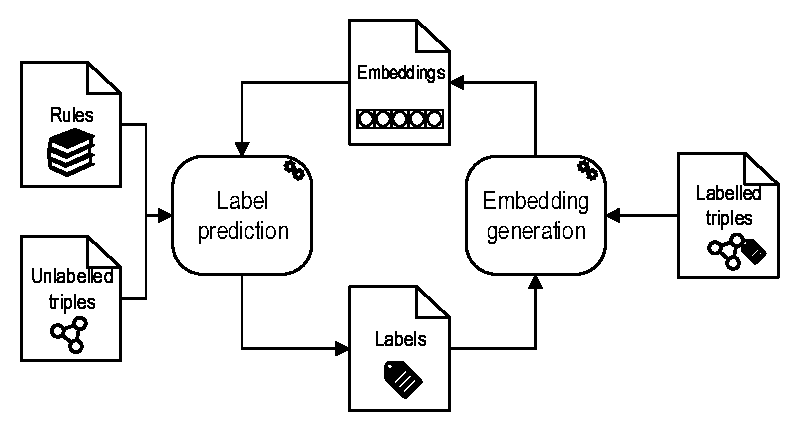
\includegraphics[width=.85\textwidth]{fig/rules/ruge}
%     \caption{Overview of the RUGE model}
%     \label{fig:rule-ruge}
% \end{figure}

% Furthermore, another aforementioned method, IterE \cite{zhang2019}, proposes a similar approach. IterE generates an initial set of entity embeddings for the Knowledge Graph. These embeddings are used to generate a set of rules, whose quality is evaluated. The best-performing rules are then used to generate new triples that are introduced in the KG, and the process starts anew by generating new embeddings that take into account the newly generated knowledge. This is shown in a graphical manner in Figure~\ref{fig:rule-itere}.

% \begin{figure}[!htp]
%     \centering
%     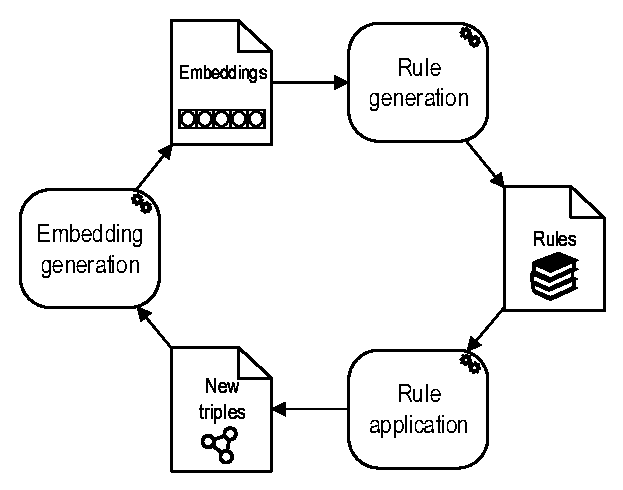
\includegraphics[width=.65\textwidth]{fig/rules/itere}
%     \caption{Overview of the IterE model}
%     \label{fig:rule-itere}
% \end{figure}

% \citet{meilicke2019} proposed AnyBURL, a technique that can generate logic rules in a bottom-up manner and on-demand. AnyBURL works by deconstructing a Knowledge Graph into a set of labeled paths. Then, it uses path-based features to determine which paths contain more useful information to obtain rules from. AnyBURL is more lightweight than other related rule-based proposals and, due to the fact that it only considers the most promising paths inside a KG, can be applied to larger graphs.

% \citet{niu2020} presented RPJE, a proposal that brings together path-based information and first-order rules. It first mines logical rules, and then uses those of length 2 to combine paths in the KG, and rules of length 1 to create a number of semantic relations.

% Finally, \citet{ma2019} introduced ELPKG, a proposal that brings together all three main approaches that we have covered in the previous chapters. It uses entity embeddings to represent the relations between entities, and a breadth-first search to detect the paths between the two entities in a triple. The information gained from both the embeddings and the paths is combined together, and it then applies soft logic to obtain the final confidence value for the triple. 

\section{Summary}\label{sec:rule-summary}
% This chapter has provided an overview of the current approaches to Knowledge Graph completion that are based on logical rules. First, we have introduced the proposals that can be found in the literature that rely solely on obtaining and applying these rules. Then, we have focused on the methods for filtering candidate triples using first-order rules. At last, we covered the methods that combine rule mining with path-based information or latent representations, such as tensors or entity embeddings.

    %%%%%%%%%%%%%%%%%%%%%%%%%%%%%%%%%%%%%%%%

    \part{Our Proposal}
    \chapter{SpaceRL: Our Knowledge graph reasoning proposal.}\label{chap:SpaceRL}

\chapterQuote{\hfill\textit{``Reason has always existed, but not always in a reasonable form.''}}{--- Karl Marx}

\chapterAbstract{H}{ere we speak about the main proposal for KG reasoning.}
% When a set of candidate triples has been obtained, the next step in Knowledge Graph completion is to classify every triple in said set to determine if it represents correct knowledge or not and, if found to be correct, added back to the KG in order to enrich it. In this chapter we introduce CAFE, our proposal for candidate triple classification. This chapter is structured as follows: Section~\ref{sec:cafe-intro} introduces it, Section~\ref{sec:cafe-proposal} presents the neighborhood-aware features that CAFE uses to discern between correct and incorrect triples, as well as the process it follows to do so, Section~\ref{sec:cafe-architecture} discusses its internal architecture and the design choices behind it, Section~\ref{sec:cafe-evaluation} shows the experiments that we carried out to assess the effectivity of CAFE, as well as their results; Section~\ref{sec:cafe-limitations} discusses its practical limitations; finally, Section~\ref{sec:cafe-summary} summarizes the chapter.

\section{Introduction}\label{sec:spacerl-intro}
% This chapter presents CAFE~\cite{borrego2021}, our proposal for triple classification. CAFE covers the second main step in Knowledge Graph completion: once an adequately small set of candidate triples has been obtained, every triple in it must be carefully evaluated to determine whether or not it represents correct knowledge and, if so, added to the KG to enrich and expand it.

% CAFE works by transforming any possible triple into a numerical vector by using a novel set of neighborhood-aware features, which measure the correctness of a triple leveraging its context in a Knowledge Graph. By transforming all triples into vectors in this manner, CAFE trains and uses a binary classifier to discern between correct and incorrect triples.

% We thoroughly evaluate CAFE using several well-known Knowledge Graphs, and our evaluation shows that it is able to achieve a high precision in challenging, real-world scenarios, thus allowing for a trustworthy KG completion process.

% Over the course of this chapter, we continue to follow the running example introduced in Section~\ref{sec:theo-intro}.

This chapter introduces SpaceRL, our Reinforcement Learning based proposal for Knoledge Graph applications. SpaceRL

\section{Formal Description}\label{sec:spacerl-formal_description}
la descripción formulomatemática del problema.

\section{Our proposal}\label{sec:spacerl-proposal}
mini resumen de lo que ofrece.
% As previously described, the second major step when completing a Knowledge Graph consists of analyzing the set of possible candidate triples, assessing which ones represent correct knowledge, and adding them back to the KG in order to augment it. In this step, it is important to achieve a high precision, in order to have a Knowledge Graph completion process that is as trustworthy as possible~\cite{shen2022overview}.

% To carry out this process, we have devised CAFE, a technique that classifies candidate triples into correct or incorrect ones. Given a Knowledge Graph and a set of candidate triples, CAFE evaluates each one of them and assigns them a binary label, denoting whether it should be considered correct and added to the Knowledge Graph, or incorrect and discarded. CAFE does this by defining a set of neighborhood-aware features, which checks for shared neighborhoods at several distance levels and under certain conditions, under the assumption that the entities in correct triples usually have a higher degree of overlap in their neighborhoods. Then, using these features, each candidate triple is converted into a numerical vector. Finally, CAFE trains a number of neural classification models using these vectors to learn to separate correct triples from incorrect ones. In the following subsections, we describe the features and architecture of CAFE in detail.

\subsection{Reinforcement Learning implementation}\label{sec:spacerl-rlimplementation}
apartado del mismo nombre del paper del eswa

hablamos de los algoritmos que utilizamos

% We propose a set of neighborhood-aware features that takes neighborhood subgraphs, reachable entities and paths into account. Due to the large number of possible variations of each feature, we present our feature set in terms of groups of features. Each group can be parameterized to obtain a specific feature, which we call an instance of the feature group.

% For the sake of example, we illustrate a possible instance of every feature group and its value using the example triple $example = $\tripleSty{(Daniel Radcliffe, plays, Harry Potter)}, and the KG shown in Figure~\ref{fig:kg-potter}.

% \featgroup{Number of entities in the neighborhood subgraph of size \texorpdfstring{$n$}{n} of the source entity in the triple.}
% {n}
% {|\Eset{}_s^n|}
% {fig:kg-potter}
% {2}
% {$|\{$\textit{Daniel Radcliffe, Harry Potter and the Goblet of Fire (movie), Harry Potter and the Prisoner of Azkaban (movie), Harry Potter and the Goblet of Fire (book), Harry Potter and the Prisoner of Azkaban (book)}$\}| = 5$}


% \featgroup{Number of entities in the neighborhood subgraph of size \texorpdfstring{$n$}{n} of the target entity in the triple.}
% {n}
% {|\Eset{}_t^n|}
% {fig:context-examples-b}
% {3}
% {$|\{$\textit{Harry Potter, J.K. Rowling, Harry Potter and the Goblet of Fire (book), Harry Potter and the Prisoner of Azkaban (book), Robin Ellacott, Hermione Granger}$\}| = 6$}

% \featgroup{Degree of N-path centrality of the source entity in the triple.}
% {n}
% {\frac{|\Eset{}_s^n|}{|\Eset| - 1}}
% {fig:context-examples-a}
% {1}
% {$|\{$\textit{Harry Potter and the Goblet of Fire (movie), Harry Potter and the Prisoner of Azkaban (movie)}$\}| / (13 - 1) = 2 / 12 \approx 0.17$}

% \featgroup{Degree of N-path centrality of the target entity in the triple.}
% {n}
% {\frac{|\Eset{}_t^n|}{|\Eset| - 1}}
% {fig:context-examples-b}
% {1}
% {$|\{$\textit{Harry Potter and the Goblet of Fire (book), Harry Potter and the Prisoner of Azkaban (book)}$\}| / (13 - 1) = 2 / 12 \approx 0.17$}

% \featgroup{Number of common entities between the neighborhood subgraph of size \texorpdfstring{$n$}{n} of the source entity and the neighborhood subgraph of size \texorpdfstring{$m$}{m} of the target entity in the triple.}
% {n, m}
% {|\Eset{}_s^n \cap \Eset{}_t^m|}
% {fig:context-examples}
% {2, 3}
% {$|\{$\textit{Harry Potter and the Goblet of Fire (book)}, \textit{Harry Potter and the Prisoner of Azkaban (book)}$\}| = 2$}

% \featgroup{Jaccard index of similarity between the entities in the neighborhood subgraph of size \texorpdfstring{$n$}{n} of the source entity and the neighborhood subgraph of size \texorpdfstring{$m$}{m} of the target entity in the triple.}
% {n, m}
% {jaccard(\Eset{}_s^n, \Eset{}_t^m)}
% {fig:context-examples}
% {2, 3}
% {$|\{$\textit{Harry Potter and the Goblet of Fire (book), Harry Potter and the Prisoner of Azkaban (book)}$\}|$~$/$~$|\{$\textit{Daniel Radcliffe, Harry Potter and the Goblet of Fire (movie), Harry Potter and the Prisoner of Azkaban (movie), Harry Potter and the Goblet of Fire (book), Harry Potter and the Prisoner of Azkaban (book), Harry Potter, J.K. Rowling, Robin Ellacott, Hermione Granger}$\}| = 2~/~9 = 0.22$}

% \featgroup{Adamic-Adar index of closeness between the neighborhood subgraphs of size \texorpdfstring{$n$}{n} of the source and target entities in the triple.}
% {n}
% {\sum_{e \in \nearby{s}{n} \cap \nearby{t}{n}}{\frac{1}{log |\nearby{e}{n}|}}}
% {fig:context-examples}
% {2}
% {$\frac{1}{log |\nearby{\textit{\footnotesize Harry Potter and the Goblet of Fire (book)}}{2}|} = \frac{1}{log |3|} \approx 2.09$}

% \featgroup{Number of reachable entities through the relation \texorpdfstring{$r$}{r} at distance \texorpdfstring{$n$}{n} from the source entity in the triple.}
% {r, n}
% {|Reachable(s, r, n)|}
% {fig:context-examples-a}
% {\textit{hasPrequel}, 2}
% {$|\{$\textit{Daniel Radcliffe, Harry Potter and the Prisoner of Azkaban (movie)}$\}| = 2$}

% \featgroup{Number of reachable entities through the relation \texorpdfstring{$r$}{r} at distance \texorpdfstring{$n$}{n} from the target entity in the triple.}
% {r, n}
% {|Reachable(t, r, n)|}
% {fig:context-examples-b}
% {\textit{created}, 2}
% {$|\{$\textit{Harry Potter,Hermione Granger, Robin Ellacott}$\}| = 3$}

% \featgroup{Number of common reachable entities through the relation \texorpdfstring{$r$}{r} from the source entity at distance \texorpdfstring{$n$}{n} and from the target entity at distance \texorpdfstring{$m$}{m}.}
% {r, n, m}
% {\\|Reachable(s, r, n) \cap Reachable(t, r, m)|}
% {fig:context-examples}
% {\textit{created}, 2, 3}
% {$|\{$\textit{Daniel Radcliffe}$\} \cap \{$\textit{Harry Potter, Hermione Granger, Robin Ellacott}$\}| = 0$}

% \featgroup{Jaccard index of similarity between the reachable entities through the relation \texorpdfstring{$r$}{r} from the source entity at distance \texorpdfstring{$n$}{n}, and those reachable through the relation \texorpdfstring{$r$}{r} from the target entity at distance \texorpdfstring{$m$}{m}.}
% {r, n, m}
% {\\jaccard(Reachable(s, r, n), Reachable(t, r, m))}
% {fig:context-examples}
% {\textit{created}, 2, 3}
% {$|\emptyset|$~$/$~$|\{$\textit{Harry Potter, Hermione Granger, Robin Ellacott}$\}| = 0~/~3 = 0$}


% \featgroup{Number of distinct paths of length \texorpdfstring{$n$}~ between the source and the target entity in the triple, using  relations \texorpdfstring{$r_1, \ldots, r_n$}{r1, ..., rn}.}
% {n, r\textsubscript{1}, \ldots, r\textsubscript{n}}
% {|\kgpathP{s}{t}{r_1,\ldots, r_n}|}
% {fig:kg-example}
% {4, \textit{starred\_in, based\_on, writer, created}}
% {$1$, as there is one path of length 4 between the entities \textit{Daniel Radcliffe} and \textit{Harry Potter} that matches the given relations}

% % Discussion of features
% The rationale behind this set of features is manifold. Regarding $f_1$ and $f_2$, knowing the size of the neighborhood of an entity can be helpful to determine whether said neighborhood encompasses relevant information. For instance, our hypothesis is that very large neighborhoods tend to contain a higher amount of unrelated information. The same idea is leveraged in $f_3$ and $f_4$, which provide normalized indices of centrality with respect to the total amount of entities in the KG. Following the previous reasoning, we hypothesize that entities with large indices of centrality (i.e. highly connected to other entities) will yield less useful information. Meanwhile, feature groups $f_5$, $f_6$ and $f_7$ measure the degree of overlap that exists in the neighborhoods of the two entities, both in absolute and in relative terms, under the assumption that correct triples have a higher degree of overlap between the neighborhoods of their entities.

% The previously discussed feature groups do not consider the specific relations involved. However, we deem it reasonable to assume that some relations may be more useful than others to determine whether a triple is correct, depending on their specific semantics. For example, having one or more children in common can be an indication of a marriage, while having the same nationality is not. In order to exploit this fine-grained information, feature groups $f_8$, $f_9$, $f_{10}$ and $f_{11}$ are similar to the previously discussed groups but restrict themselves to only one relation. These groups are computed for every relation in a KG.

% Finally, feature group $f_{12}$ allows CAFE to find the number of paths that exist between two entities for any given relations. It is our intuition that correct triples have more alternative paths between the two entities they contain than false ones.

\subsection{Reward structure}
mencion a las posibles recompensas implementadas en la herramienta.
% Our proposal, CAFE, receives a KG and a set of relations from that KG as input, and outputs a classification model for each of the provided relations. These models are able to determine if a given triple that represents an instance of the relation is correct and should belong to the KG. Its workflow is depicted in Figure~\ref{fig:workflow-cafe} and, in the following, we describe each of its steps.

% \begin{figure}[htp]
%     \centering
%     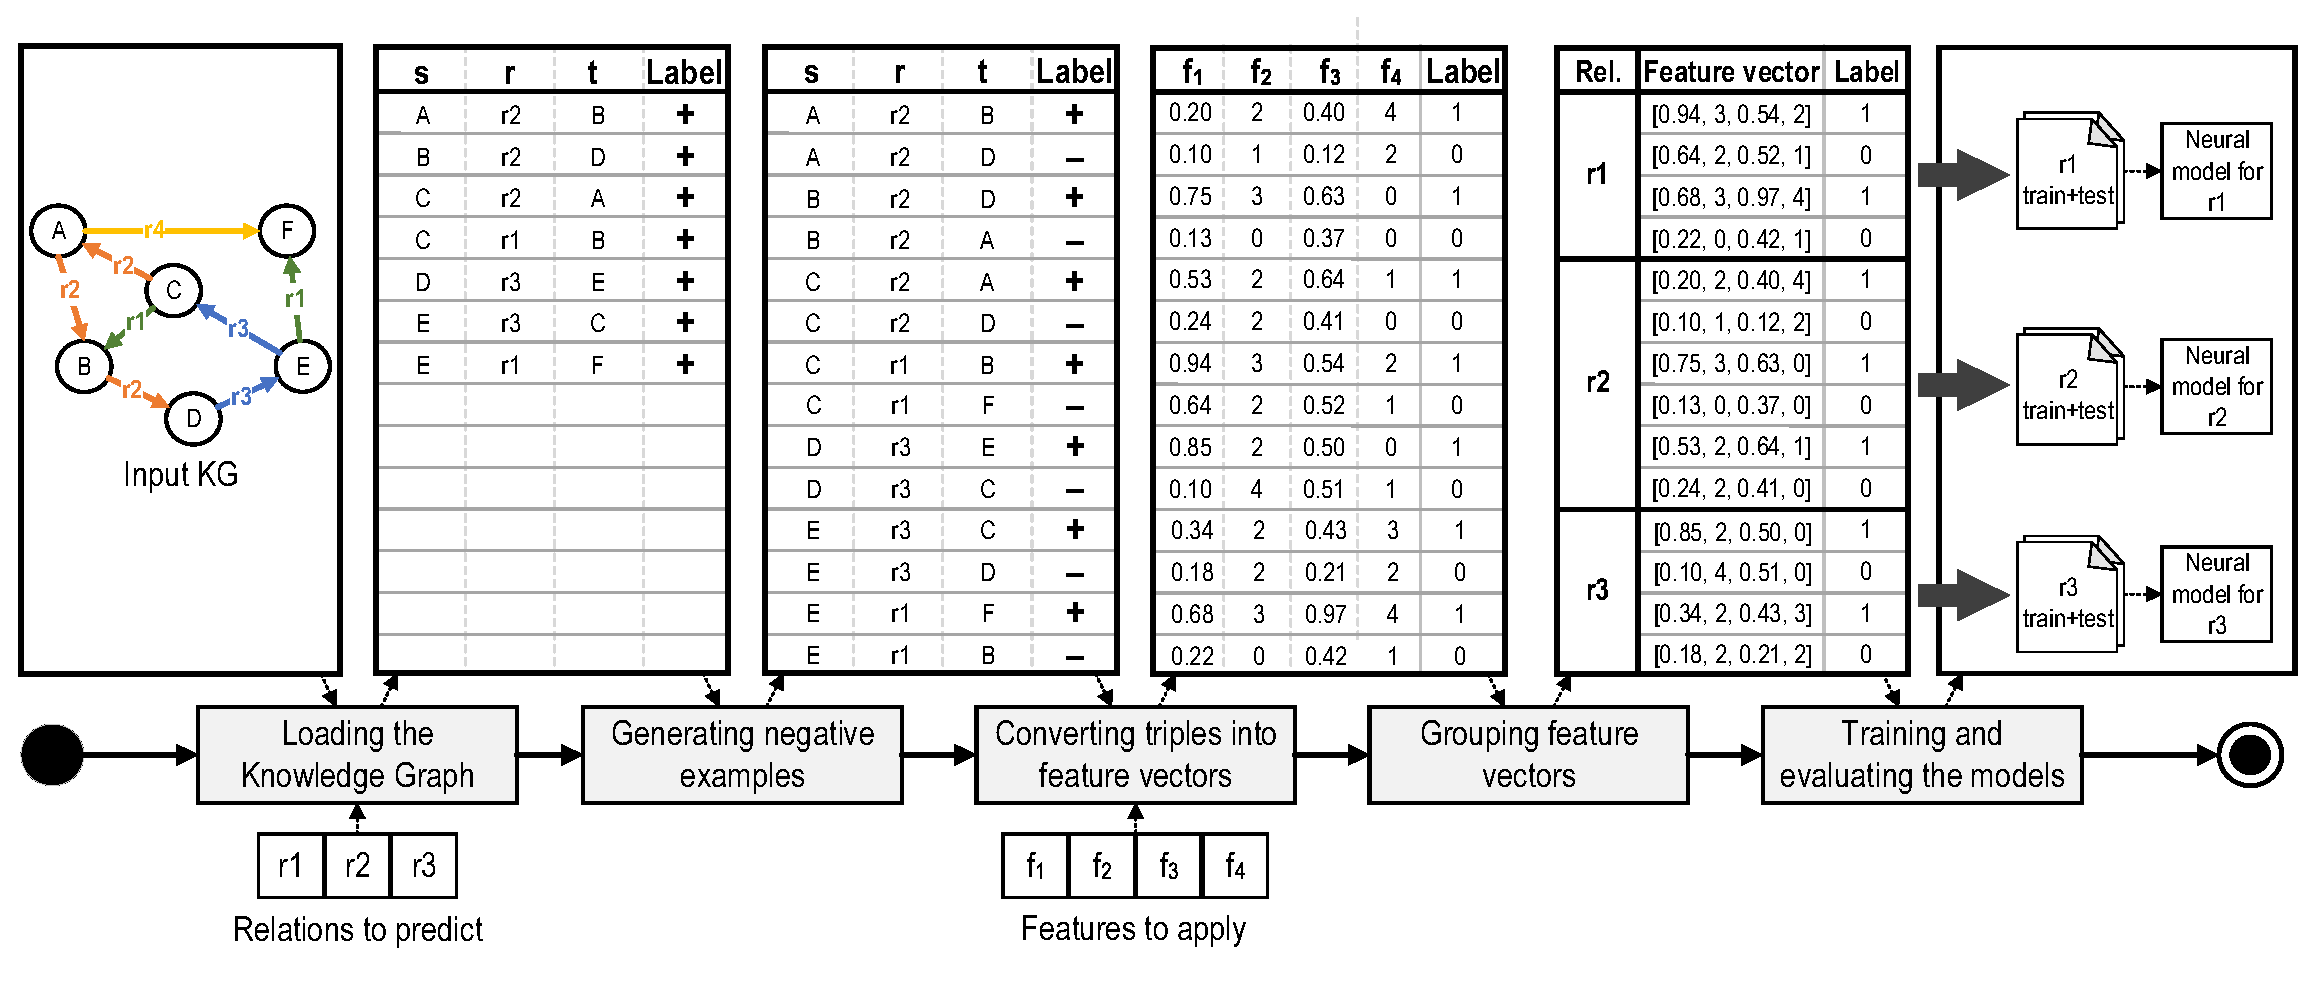
\includegraphics[width=\textwidth]{fig/cafe/workflow}
%     \caption{In-depth view of the CAFE workflow}
%     \label{fig:workflow-cafe}
% \end{figure}

% \begin{itemize}
%     \item \textbf{Loading the Knowledge Graph:} CAFE internally stores the input KG in the form of \triple{} triples, using an efficient data structure based on hash tables, which is suitable for a high frequency of read operations due to its O(1) lookup times. The triples that contain relations for which a predictive model does not need to be generated are still taken into account when computing features, since they may provide valuable predictive information, but they are not transformed into feature vectors in the following steps.\\
    
%     \item \textbf{Generating negative examples:} A Knowledge Graph contains only positive information, i.e., it contains examples of the occurrence of a relation $r$ between two entities. However, it does not contain explicit information about pairs of entities for which $r$ does not hold. Our proposal relies on a classification model that requires negative examples for training, which means that a number of negatives for each positive triple must be produced. To accomplish this, we follow the type-constrained local closed world assumption \cite{bansal2020negatives}, i.e., we generate negative examples from every triple \triple{} present in a KG by replacing their target entity $t$ with a different one, $t'$, such that the resulting triple \negtriple{} does not exist in the KG. Furthermore, to preserve the range of each relation, we randomly choose $t'$ such that there exists some other triple in the KG where $t'$ appears as the target entity for the relation $r$. This is known as type constraint.\\

%     In the example depicted in Figure \ref{fig:kg-potter}, a valid negative example is \tripleSty{(Hermione Granger, appears\_in, The Cuckoo's Calling)}, since we know that \tripleSty{The Cuckoo's Calling} is a valid target for the relation \tripleSty{appears\_in}. However, \tripleSty{(Hermione Granger, appears\_in, Daniel Radcliffe)} would not be allowed as a negative example, because \tripleSty{Daniel Radcliffe} never appears as the target of the relation $appears\_in$.\\
    
%     It can be argued that generating negative evidence in this manner can produce false negatives by mere chance, i.e., statements that are deemed incorrect but that are true in the real world. While this is indeed plausible, it is generally accepted~\cite{ji2015, lin2015, socher2013} that the chances of this happening are very low and, as a consequence, the possible effects on the final results are not significant.\\

%     \item \textbf{Converting triples into feature vectors:} Once negative examples have been generated, our feature set is instantiated and applied to all triples. For all feature groups, we obtain all possible feature instances by applying all possible combinations of the values of their parameters. Each feature instance assigns a real number to each triple. Therefore, applying several features to a triple results in a feature vector. Each position of the feature vector represents that real number that the corresponding feature assigned to the triple.\\

%     It is important to note that, to compute features on a positive training triple, we temporarily remove it from the KG, since not doing so would result in trivial prediction models such as ``a person plays a character if there exists a triple in the KG stating that the person plays that character''.\\\newpage

%     \item \textbf{Grouping feature vectors:} The previous step computes feature vectors of triples. Since these triples can be either positive or negative, the feature vectors are accordingly labeled as positive or negative. Based on the labeled feature vectors, we train a classification model for each relation that predicts whether a triple should be added to the KG. We do this in order to allow the models to capture meaningful and distinctive information for every relation: even though the same set of features is applied to all triples, some features might have more predictive power for a relation, and other features may be more helpful for a different one.\\
    
%     \item \textbf{Training and evaluating the models:} For every relation that we predict, we create one or more neural models, where each model focuses only on the features that are obtained from a certain neighborhood size. Thus, using only neighborhood subgraphs of size 1 results in one model, using neighborhood subgraphs of size of up to 2 results in two models, and so on. This allows each model to capture the specific information that every neighborhood size may yield. To combine two or more models, we use an additional combination layer to produce a single output.

%     The neural models are trained using the labeled feature vectors in the training split for the desired relation, where each model receives only the features corresponding to its assigned neighborhood size, and the label or ground truth is shared among them. Prior to training our models, we first remove any individual features that have the exact same value in every feature vector and thus lack any predictive power. An example of this are path-based features ($f_{12}$), since only a small subset of all possible paths of fixed length occur between two given entities, and as a consequence most of them have a value of 0.
    
%     It is important to note that we use neural classification models because they have been shown to consistently achieve satisfactory results in many different classification tasks~\cite{aggarwal2012, yadav2019, ayala2020}, although other classification models that make use of our features could be used in this step.
% \end{itemize}

\section{Policy Network}\label{sec:spacerl-policy}
aqui hablamos de la policy que hemos usado y porque consideramos que es buena practica las LSTM...

% We show the internal class architecture of CAFE in Figure~\ref{fig:cafe-diagram}, and its data workflow is displayed in Figure~\ref{fig:cafe-flow}. We further describe and discuss the architecture of CAFE in the following.

% \begin{figure}[!htp]
%     \centering
%     \includesvg[width=1.0\textwidth]{fig/cafe/CAFE-classes}
%     \caption{Architecture of CAFE}
%     \label{fig:cafe-diagram}
% \end{figure}

% \begin{figure}[!htp]
%     \centering
%     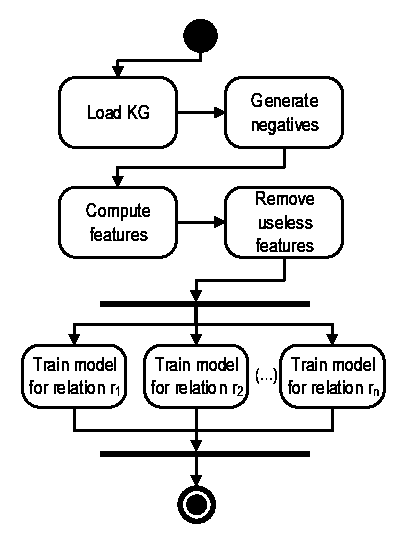
\includegraphics[width=.45\textwidth]{fig/cafe/CAFE-flow}
%     \caption{Workflow of CAFE}
%     \label{fig:cafe-flow}
% \end{figure}

% The main flow of CAFE is coordinated by the class \textit{ParallelWorker}. This class can be configured to use a certain number of threads, and then internally spawns processes to parallelize the different tasks done by CAFE. This is done by splitting the total number of triples in the KG between the different threads, since the processing of triples can be done concurrently for the most part, as shown in Figure~\ref{fig:cafe-flow}. 

% The method \textit{genNegs} produces negative triples using the \textit{NegativeGenerator} class and a generation strategy, since they are necessary to train the classification models.

% Then, the method \textit{compFeats} transforms every triple in the KG into a labeled feature vector, using a series of neighborhood-aware features that leverage the similarities of the neighborhoods of two entities in a KG. This is done by measuring the similarities of the entity neighborhoods of the source and target of a triple, using measures such as the Jaccard index of similarity, analyzing the size of such neighborhoods using measures such as the Adamic-Adar index; as well as assessing the overall connectivity of the entities of a triple using the N-path centrality index.

% The method \textit{filtFeats} removes the features that have the same value in all labeled vectors, since they have no predictive power. Finally, method \textit{getClassifier} trains and returns a neural classifier for a given set of labeled vectors, corresponding to a certain relation in the KG. Given that the work done by these methods is usually carried out in an independent manner for each triple, it is parallelized among different execution threads.

% Class \textit{ParallelWorker} uses other classes by means of composition to perform specialized tasks: Class \textit{NegativeGenerator} provides a unified interface to easily generate a negative triple in a KG following one of the available strategies, which are implemented using \textit{NegGenerationStrategy} classes.

% Class \textit{KGLoader}, through its \textit{load} method, is used to read and write KGs in different formats, namely: N3, Turtle, and RDF/XML.

% Class \textit{FeatureVectorCalculator} is responsible for applying the previously discussed catalogue of features to any given triple using the method \textit{getVec}, resulting in a labeled vector for that triple. The catalogue of available features can be easily expanded thanks to the \textit{Feature} class, since each individual feature is implemented as an instance of that class.

% Class \textit{FeatureFilterer} specializes in removing useless features from a feature vector, i.e., those that share the same value in all vectors and thus have no predictive power. Method \textit{filtFeat} receives the labeled vector to be processed and a set of all other labeled vectors, to allow for the multithreaded processing of different labeled vectors simultaneously.

% Finally, the \textit{NeuralClassifier} class produces, trains and evaluates the neural models that determine whether a triple is correct. These models receive as input the feature vector generated from the triple in question, and outputs a confidence value between 0 and 1. The models used by CAFE have three feed-forward layers with 1024, 512 and 256 neurons each. The method \textit{initialize} produces a new model for a certain relation, to allow it to specialize in the specific details of said relation, which may be different to other relations present in the KG. The method \textit{train} receives the training set of labeled vectors resulting from processing a KG with the \textit{ParallelWorker}, and uses them to train the classification model. This method uses a learning rate of 0.001, a dropout of 0.1 for all layers, a batch size of 16 and 100 epochs, as these parameters have been proven to yield satisfactory results in some of our previous work \cite{borrego2021}. Then, all vectors in the testing set are evaluated using the \textit{predict} method.

% Throughout the whole process, the \textit{Settings} class is queried to retrieve the configuration parameters set by the user, e.g., the relative sizes of the training and testing splits, or the negative generation strategy to use.

% CAFE has two main dependencies with external libraries: NetworkX \cite{hagberg2008networkx}, which is used to internally store the KG and apply graph-based algorithms to compute the different features; and TensorFlow \cite{tensorflow2015}, which is used to create, train and apply the neural classification models.

% \subsection{Design and performance considerations}
% The architecture of CAFE shares some common patterns and design decisions with that of CHAI, described in the previous chapter. Most classes only need to be instantiated once throughout the execution of CAFE and, for this reason, we have decided to turn them into singletons for simplicity of use and to minimize the use of memory.

% There are, nonetheless, a number of classes that clearly must allow multiple instances of them to exist, in order to represent variations of the same concept. A prime example of this is the Feature class: all features share the same interface, since they receive a triple and the KG that contains it and produces a numeric value. However, in order to accommodate all features defined in Section~\ref{sec:cafe-features}, each one of them exists as an instance of Feature.

% Another example is the possible existence of multiple negative generation strategies, where one must be chosen at runtime according to the selection of the user. In both cases, they are accessed through auxiliary classes that act as catalogues, automatically detecting and loading all instances of the catalogued classes. 

% Given that CAFE is a very computationally intensive system, several optimizations have been made to make the best possible use of the resources of the system it runs on. Due to the fact that computing a feature vector for a triple can be done independently of all other triples in a KG, this task is parallelized and evenly distributed among all available cores in a CPU. This, however, comes at the cost of ensuring that all singletons in the system are thread-safe, given that they will be accessed by multiple processes at the same time.

% Finally, it is important to note that all features defined by CAFE are deterministic, and will always return the same value for the same triple in a KG. Most features only analyze one of the entities in a triple at a time, and thus are re-computed very often for the same entity. For this reason, we have implemented a thread-shared caching strategy, in which the result of applying a feature to a triple is stored into a cache that is accessed by all threads. This allows CAFE to significantly reduce the number of calculations that must be performed when processing a KG.

\section{Evaluation}\label{sec:spacerl-evaluation}
estructura de evaluacion similar a la vista en otras tesises.
se puede casi que calcar tal cual del paper del eswa y plantarlo aqui con unas modificaciones pequeñas.
% In this section, we present the evaluation that we carried out to assess the performance and effectiveness of CAFE. First, we introduce the Knowledge Graphs on which CAFE was applied and an overview of their main characteristics. Next, we explain the methodology that we used to evaluate CAFE. Finally, we show and discuss the results of our evaluation.

\subsection{Experimental data}
% We evaluated our proposal using four KGs provided by the freely available AYNEC-DataGen~\cite{ayala2019} tool: FB13-A, WN11-AR, WN18-AR and NELL-AR. These KGs are based on the well-known FB13, WN11 \cite{socher2013}, WN18~\cite{bordes2014}, and a subset of NELL proposed in \cite{gardner2015}. However, they have been processed to remove reciprocal relations detected by AYNEC, i.e., relations $r$ and $r'$ such that, if $(s, r, t)$ exists, then $(t, r', s)$ also exists very frequently. Additionally, relations that amount to less than 5\% of the total number of triples in the graph have been removed.

% These evaluation KGs originally contained one negative example per each positive triple in both their training and testing splits. In order to study how the KG completion techniques perform when presented with a much higher volume of negative evidence, we created versions of these graphs whose testing splits contained 10 negative examples per positive, using the AYNEC-DataGen tool. We believe that this is a more realistic scenario, since a much higher number of negative examples per positive triple is typically expected in real-world KG completion tasks~\cite{borrego2019}. To avoid confusion, we denote these versions as FB13-A-10, WN11-AR-10, WN18-AR-10 and NELL-AR-10.

% For FB13-A-10, WN11-AR-10 and WN18-AR-10, we aimed to predict all possible relations, and for NELL-AR-10 we focused on the same subset of 10 relations that were used to evaluate SFE~\cite{gardner2015}. However, in the latter KG, one relation was removed by AYNEC for being the reciprocal of another relation, leaving 9 relations for evaluation. In the specific case of FB13-A-10, we transferred 25\% of the training triples over to the testing set in order to provide testing examples for some relations, as they were not available in the original KG as introduced in \cite{socher2013}. Table \ref{table:cafe-datasets} provides an overview of the aforementioned KGs. In the case of NELL-AR-10, we show in parentheses the amount of triples and relations that were considered for evaluation, although the entire graph was used for computing features.

% \begin{table}
    % \footnotesize
    \begin{center}
    \begin{tabular}{ >{\raggedright\arraybackslash}M{3.5cm} | M{2.5cm} | M{2.5cm} | M{1.75cm} | M{1.75cm} }
    \centering \textbf{KG} & \textbf{Training triples} & \textbf{Test triples} & \textbf{Entities} & \textbf{Relations} \\
    % actualizado marzo 2021
    \hline
    FB13-A-10 & 228,172 & 481,457 & 74,998 & 13 \\ 
    \hline
    WN11-AR-10 & 77,948 & 198,231 & 38,195 & 9 \\
    \hline 
    WN18-AR-10 & 71,984 & 183,051 & 40,943 & 11 \\
    \hline 
    NELL-AR-10 & 86,971 (1,451) & 219,374 (5,083) & 53,934 & 148 (9) \\
    \end{tabular}
    \caption{Overview of the KGs used for evaluating CAFE}
    \label{table:cafe-datasets}
    \end{center}
\end{table}

\subsection{Experimental setup}
% A neural prediction model was created for every relation of interest and trained using its corresponding training set. Then, the model was applied to all feature vectors in the test set, and we compared the expected label (which denotes whether it represents a correct triple or not) against the label that was produced by our model. We report our results in terms of precision, recall and F1, in order to determine how effective our proposal is when determining the correctness of a given triple.

% We evaluated three versions of CAFE, denoted CAFE$_1$ to CAFE$_3$, which were limited to using feature instances that exploited neighborhood subgraphs and paths of a maximum size of 1, 2, and 3, respectively. This was done in order to study how using larger neighborhoods affects the effectiveness of CAFE.

% There exist many different KG completion proposals, and they often use different evaluation metrics \cite{speranskaya2020}. Due to this, it is very difficult to perform a comparison across a large number of them in a manner that is fair and rigorous. For this reason, we used TransE~\cite{bordes2013}, TransD~\cite{ji2015}, TransH~\cite{wang2014}, TransR~\cite{lin2015}, Analogy~\cite{liu2017}, SimplE~\cite{kazemi2018} and RotatE~\cite{sun2019} as baselines for our evaluation, since they are some of the most well-known state-of-the-art KG completion proposals. In order to provide a common evaluation environment for these different proposals, we used the OpenKE \cite{han2018} framework to train and evaluate these proposals using the previously discussed Knowledge Graphs. Additionally, since these proposals usually report metrics like MRR and Precision@N, we used the utilities provided by OpenKE to obtain binary labels for the testing triples, by setting a likelihood threshold in a way that optimized the classification results.

% We selected the following values for the hyperparameters of our neural models: 3 layers with 1024, 512 and 256 neurons each, learning rate of 0.001, batch size of 16, dropout of 0.1 for all layers, 100 epochs and validation ratio of 10\%. When two or more models were to be combined, we joined their results using a hidden layer with 3 neurons and an output layer with a single neuron. These values for the hyperparameters were chosen using a hold-out or ``dev'' set for the FB13-A-10 KG, and all KGs were then evaluated using the same hyperparameters. We chose them because they provided satisfactory results in our empirical tests.

% All our experiments were conducted on a computer equipped with an Intel Core i9-9900K CPU, 32GB of RAM and an Nvidia RTX 2080 Ti GPU.

\subsection{Results and discussion}
% In Figure \ref{fig:cafe-boxes}, we show the evaluation results for CAFE$_1$, CAFE$_2$, CAFE$_3$, and the related state-of-the-art proposals. For the sake of clarity, this Figure only displays the F1 values for each technique. Additionally, Table \ref{fig:cafe-table-results} shows the detailed results for all relations in every KG and for all metrics under evaluation.

% \begin{figure}[!htp]
%     \centering
%     \def\subfigscale{0.6\textwidth}
    
%     \subfigure[FB13-A-10]{
%         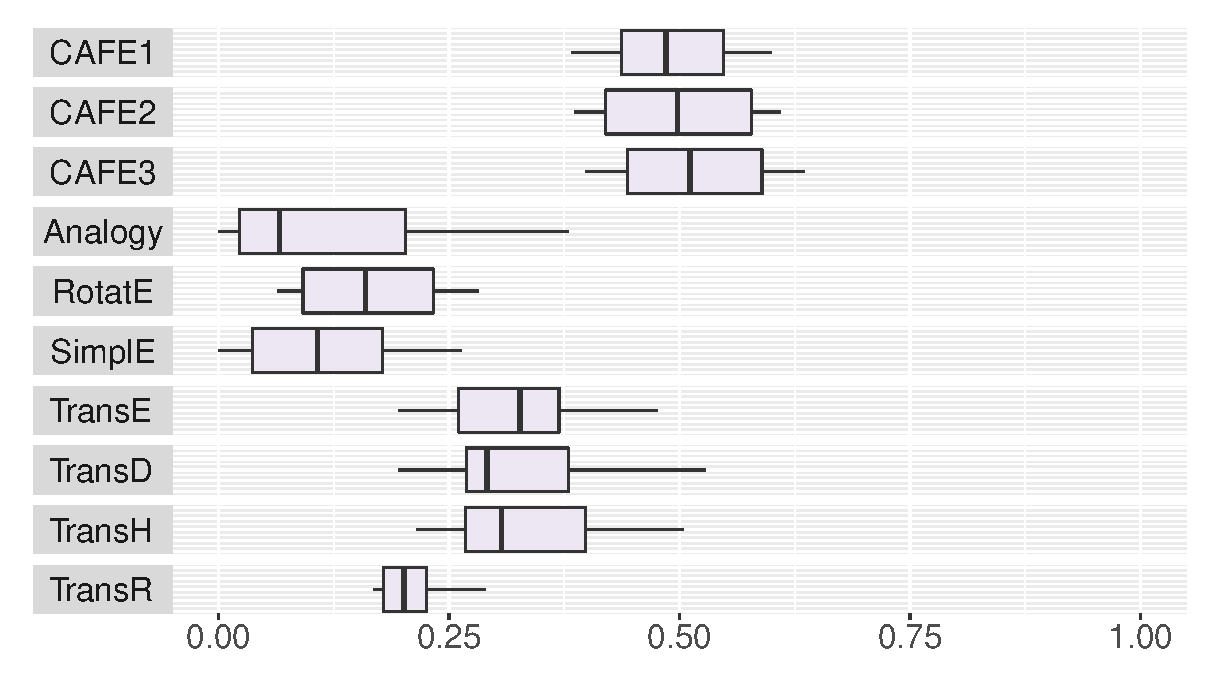
\includegraphics[width=\subfigscale]{fig/cafe/boxes/FB13-A-10}
%         \label{fig:box-FB13-A-10}
%     }\\
%     \subfigure[NELL-AR-10]{
%         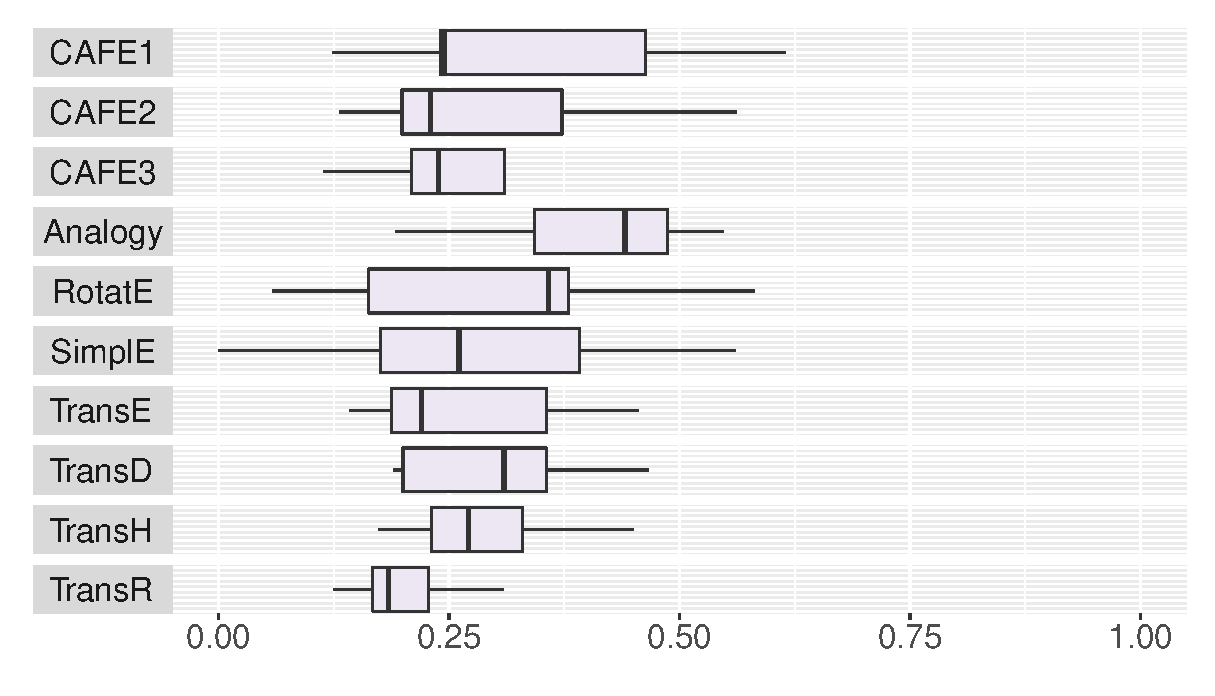
\includegraphics[width=\subfigscale]{fig/cafe/boxes/NELL-AR-10}
%         \label{fig:box-NELL-AR-10}
%     }\\
%     \subfigure[WN11-AR-10]{
%         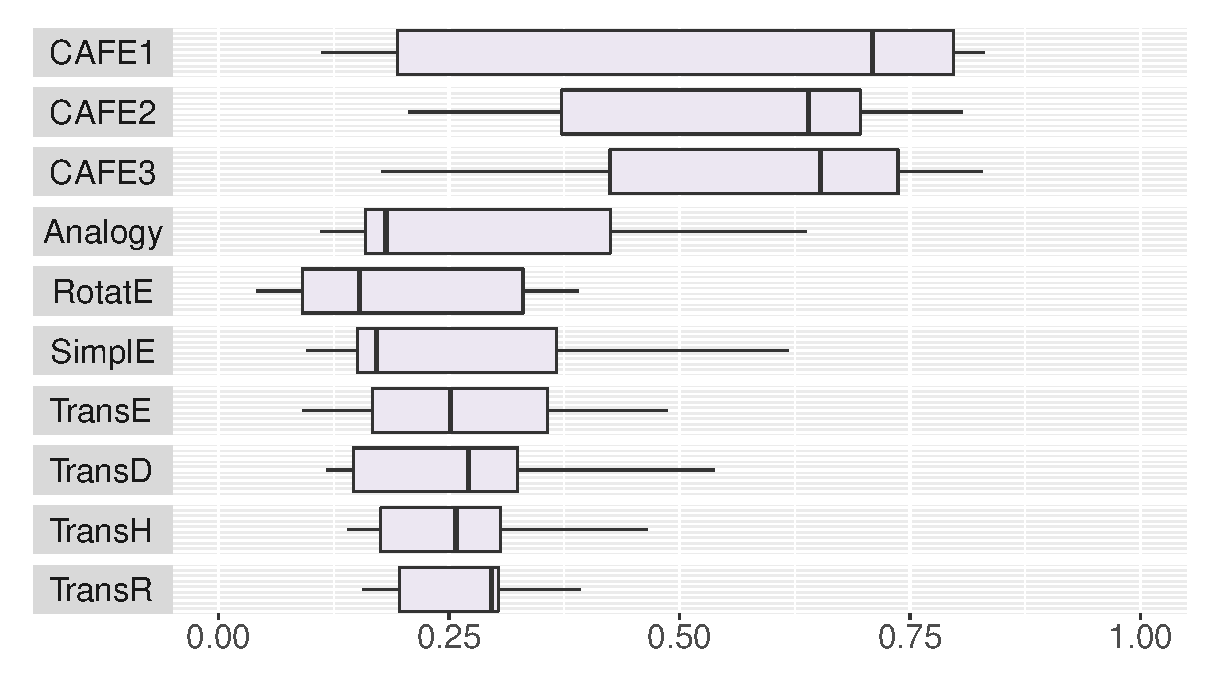
\includegraphics[width=\subfigscale]{fig/cafe/boxes/WN11-AR-10}
%         \label{fig:box-WN11-AR-10}
%     }

%     \caption{F1 comparison between CAFE and other proposals}
%     \label{fig:cafe-boxes}
% \end{figure}

% \begin{figure}[!htp]\ContinuedFloat
%     \centering
%     \def\subfigscale{0.6\textwidth}
    
%     \subfigure[WN18-AR-10]{
%         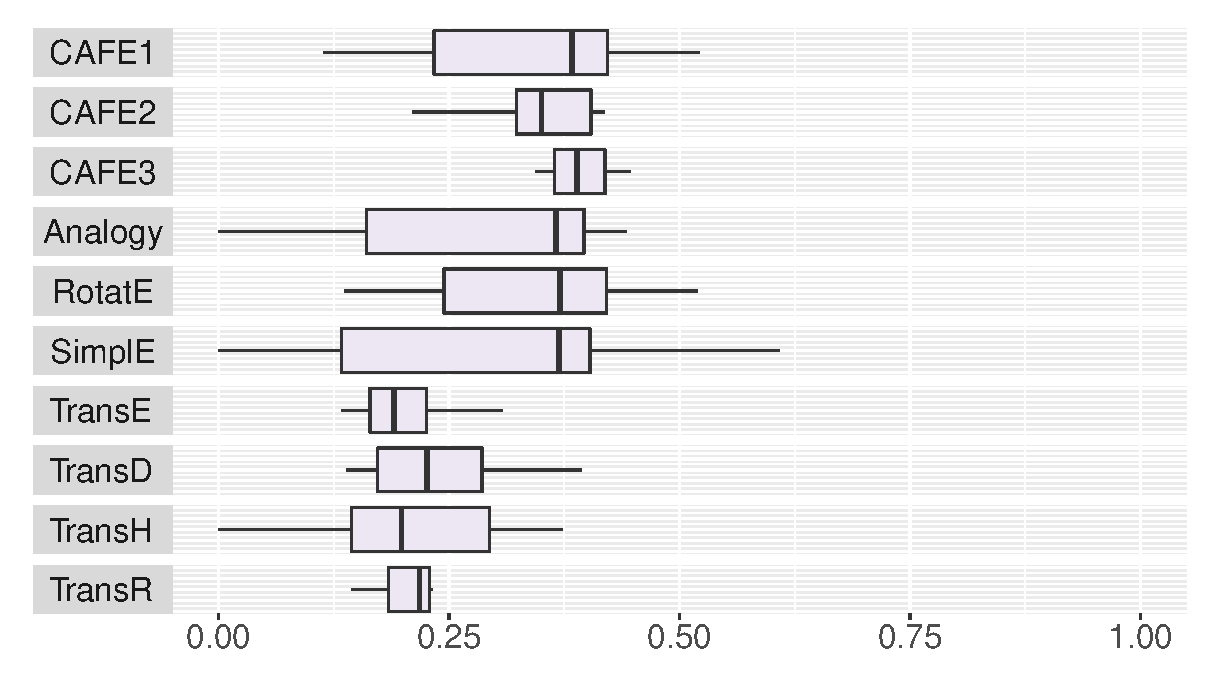
\includegraphics[width=\subfigscale]{fig/cafe/boxes/WN18-AR-10}
%         \label{fig:box-WN18-AR-10}
%     }\\
    
%     \caption{F1 comparison between CAFE and other proposals (cont.)}
% \end{figure}

% \begin{figure}[!htp]
%     \centering
%     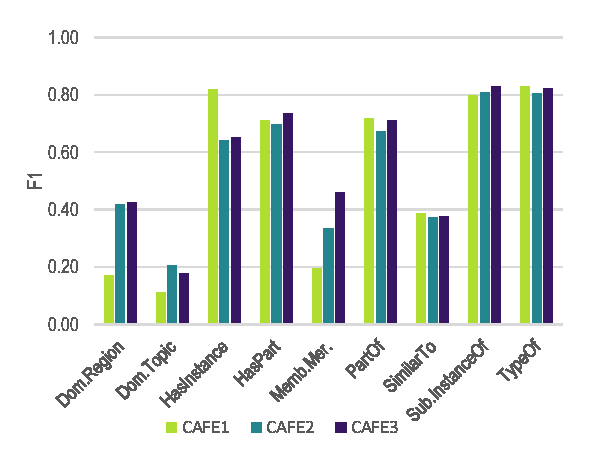
\includegraphics[width=.75\textwidth]{fig/cafe/wn11_bars}
%     \caption{F1 scores in the WN11-AR-10 KG}
%     \label{fig:cafe-wn11-bars}
% \end{figure}

% Our results show that CAFE is able to match the performance of state-of-the-art proposals, and in many cases achieve higher values on the metrics under evaluation. In the cases of FB13-A-10 (Figure \ref{fig:box-FB13-A-10}) and WN18-AR-10 (Figure \ref{fig:box-WN18-AR-10}), CAFE can reach or surpass the F1 scores achieved by other proposals in a consistent manner. CAFE also provides better results in the WN11-AR-10 (Figure \ref{fig:box-WN11-AR-10}) KG, although with a higher degree of variability, and matches the performance of the rest of the analyzed techniques in the NELL-AR-10 (Figure \ref{fig:box-NELL-AR-10}) KG. These results show that CAFE can be more effective than other proposals in challenging classification scenarios.

% \newpage
% \clearpage

% \begin{table}[H]
%     \centering
%     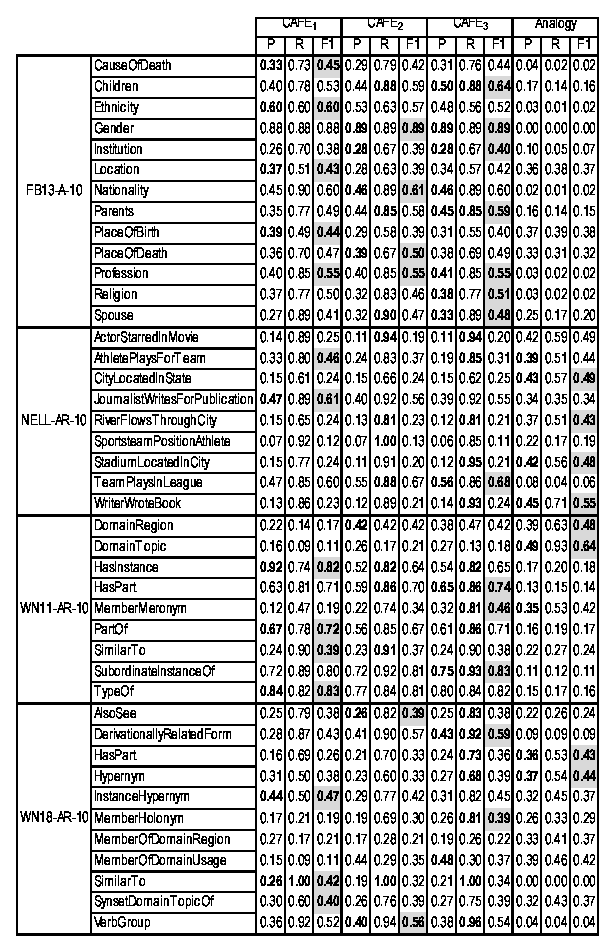
\includegraphics[height=0.8\paperheight,right]{fig/cafe/table-cafe-left}%
%     \caption{Detailed CAFE results}
%     \label{fig:cafe-table-results}
% \end{table}  
% \begin{table}[H]\ContinuedFloat
%     \centering
%     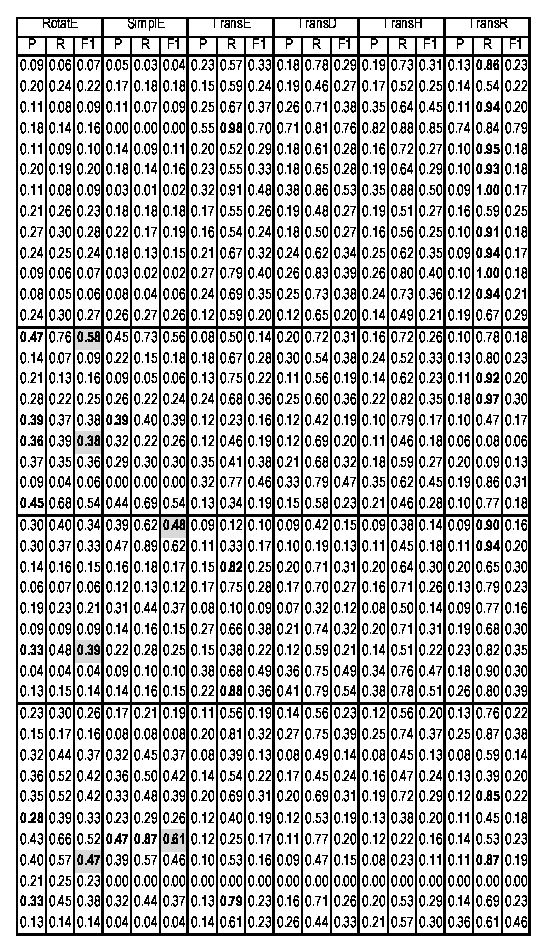
\includegraphics[height=0.8\paperheight,left]{fig/cafe/table-cafe-right}%
%     \caption{Detailed CAFE results (cont.)}
% \end{table}


% \newpage

% Table \ref{fig:cafe-table-results} displays that, in general, both a satisfactory precision and recall can be achieved, and thus we consider that CAFE is generally effective. However, there exists a number of relations for which a very high precision value is obtained at the expense of a lower recall or vice-versa, resulting in a typical precision-recall trade-off. We also observe that the nature of every individual relation has a significant impact in the results, since some of them are harder to predict than others. Such is the case of the relation \textit{cause\_of\_death}, since learning to predict the cause of the death of a person with a very high effectiveness would be a remarkable achievement that unfortunately falls out of the scope of this work. We further discuss this limitation in Section \ref{sec:cafe-limitations}.

% Regarding the question of how using different neighborhood sizes affects the effectiveness of CAFE, Figure~\ref{fig:cafe-boxes} shows that the metrics under evaluation are generally higher for CAFE$_2$ than for CAFE$_1$, but the same cannot always be said for CAFE$_3$ and CAFE$_2$. Indeed, metrics appear to remain stagnant or even decrease when using larger neighborhoods in some cases. For example, in FB13-A-10 (Figure \ref{fig:box-FB13-A-10}), we do not observe a significant increase in effectiveness when using larger neighborhood subgraphs, which suggests that the most useful information is readily available in the immediate vicinities of the relevant entities. In the cases of WN11-AR-10 (Figure \ref{fig:box-WN11-AR-10}) and WN18-AR-10 (Figure \ref{fig:box-WN18-AR-10}), an improvement is observed when using neighborhoods of size 2, but further expanding the neighborhood size does not seem to have a significant impact. A possible conclusion for this is that, at a certain point, larger neighborhood subgraphs do not provide additional value or predictive power over smaller ones. In a worst-case scenario, the number of features with little to no predictive power would greatly increase by using larger neighborhood sizes, negatively affecting the results. This effect actually occurs in the case of the NELL-AR-10 KG (Figure \ref{fig:box-NELL-AR-10}), where effectiveness decreases when increasing the size of the neighborhood subgraphs for which we compute features. A plausible explanation for this is that it has been noted that NELL contains noisier data~\cite{paulheim2014}, and thus taking larger neighborhoods into account significantly increases the amount of noise that our classification model has to deal with, reducing its effectiveness.

\section{Limitations}\label{sec:spacerl-limitations}
el apartado de conclusions y future work tiene mucho de lo que podemos poner aqui tambien.
% Despite our triple classification proposal being generally effective, it has some limitations. It does not work well for relations for which useful predictive information cannot always be found in the neighborhoods of the entities in a triple. In this regard, we identify two types of relations: those that can be predicted using other information present in the KG, and those for which the entities and relations in their neighborhoods do not provide useful information, and thus are much harder to predict. This dichotomy can be observed in the results shown in Table \ref{fig:cafe-table-results}, and it is especially notable in the WN11-AR-10 KG. For the sake of visualization, we display the results of applying CAFE to this Knowledge Graph in Figure~\ref{fig:cafe-wn11-bars}.

% This difference is particularly visible in the \textit{Similar to} and \textit{Domain topic} relations, which have low F1 scores. Upon manual inspection, we found that \textit{Similar to} tends to link words that are generally isolated within the KG and share very little common context. Also, \textit{Domain topic} is extremely broad, causing the two entities in a triple to have few or no relevant common elements in their neighborhoods, e.g., (\textit{Britain}, \textit{Domain topic}, \textit{Surgery}).

% In other cases, even if some information is present in the neighborhoods under consideration, it may be not successfully captured by CAFE due to the large amount of irrelevant data surrounding it. In this regard, the NELL-AR-10 KG shows that larger neighborhood sizes are not always better for predictive purposes, since the amount of noise they may include can be detrimental for the performance of CAFE. This can be due to some source or target entities being present in many triples (for example, countries). Therefore, larger neighborhoods of these entities introduce many other entities that are not relevant to the triple under evaluation. In these cases, it is up to the users to decide which maximum neighborhood size best caters to their interests.

\section{Summary}\label{sec:cafe-summary}

% In this chapter we have introduced CAFE, our proposal to classify candidate triples for Knowledge Graph completion. CAFE defines a set of neighborhood-aware features which evaluate several aspects of a triple, by checking for shared neighborhoods at several distances with other triples in a KG, and then combines the values of all features into a feature vector. Once all candidate triples have been transformed into feature vectors, CAFE trains and applies a neural binary classifier to discern between correct and incorrect triples, and provides the user with a set of correct candidate triples to add back to the KG. Our experimental evaluation shows that CAFE is very effective, outperforming other state-of-the-art approaches in a number of well-known Knowledge Graphs of different sizes and domains.

    \chapter{SpaceRL framework}\label{chap:framework}

\chapterQuote{\textit{``Most problems can be solved using algebra, or violence.''}}{--- Bill Wurtz}

\chapterAbstract{E}{n esta seccion podemos hablar sobre la importancia de la replicabilidad de la experimentacion pero tambien de crear herramientas accesibles para todo el mundo y no limitar el acceso solo a los expertos de dominioy ya luego meter todo lo que se ha hecho.}

% efore we delve into the details of our proposal, it is important to establish a common and unambiguous vocabulary. For this reason, we have devised a conceptual framework that allows us to describe a number of relevant concepts in detail. The chapter is organized as follows: Section \ref{sec:theo-intro} introduces it, Section \ref{sec:theo-triple} models the concept of a triple, Section \ref{sec:theo-kg} presents the theoretical model of a Knowledge Graph, Section \ref{sec:theo-paths} introduces topology-based elements such as paths, distances and reachability, Section \ref{sec:theo-subgraph} illustrates the concept of neighborhood subgraphs, Section \ref{sec:theo-candidates} presents the notions of candidate triples and candidate-filtering fitness, Section \ref{sec:theo-rule} describes candidate-filtering criteria and rules, and Section \ref{sec:theo-features} introduces graph-based features and feature groups; finally, Section \ref{sec:theo-conclusion} summarizes the chapter.

\section{Introduction}\label{sec:framework-intro}
% Throughout our proposal, we use a number of concepts, both established in this field and novel. In this chapter, we define their foundations, such as tuples of entities and relations known as triples, or the fields of a Knowledge Graph, which allow us to accurately describe further concepts. We also define paths inside a Knowledge Graph, which are the basis for many of the elements in our proposal. Building upon the notion of a path, we provide a formal definition of the distance between two entities in a Knowledge Graph, as well as of the concept of entity reachability.

% Furthermore, in this chapter, we define neighborhood subgraphs, which are portions of a KG that contain the elements most closely related to a given entity. Then, we introduce candidate triples, which are combinations of entities and relations that have a high likelihood of representing correct knowledge. To measure the tentative aptness of a candidate triple, we present the idea of candidate fitness. In order to rule out those candidate triples with a low fitness, we define candidate filtering criteria and rules. Finally, we introduce a way to numerically model a triple in a KG through the use of graph-based feature groups.

% \begin{figure}[htp]
%     \centering
%     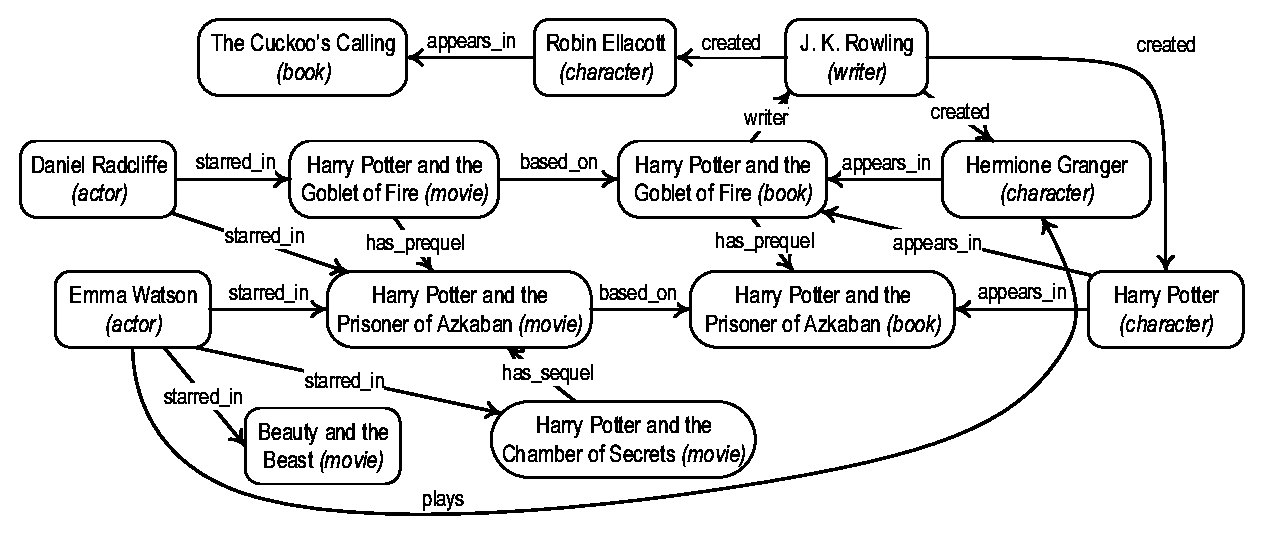
\includegraphics[width=\textwidth]{fig/theoretical/kg-harry-potter}
%     \caption{Sample KG describing works, actors, writers and characters}
%     \label{fig:kg-potter}
% \end{figure}

% To help illustrate some concepts in this chapter, Figure~\ref{fig:kg-potter} presents a KG that contains information about fictional works, actors, writers and characters.

\section{Software description}\label{sec:framework-software}
an overview of the core elements of the framework.
% The notion of a triple is pivotal to Knowledge Graphs, since it constitutes an atomical amount of structured information. A triple is a 3-tuple that contains two entities, commonly denoted \textit{source} and \textit{target}\footnote{Other literature sometimes refers to the two entities in a triple as \textit{head} and \textit{tail} \cite{dessi2022cskg,dessi2020aikg,bordes2013}, or \textit{subject} and \textit{object} \cite{nickel2016, balazevic2019,trouillon2016}.}; connected by means of a relation. This, in turn, represents a fact in a given domain.

% Formally, a triple is defined as follows:

% \defin{Triple}{
%     Let \Eset{} be a set of entities, and let \Rset{} be a set of relations. We define a triple as a 3-tuple that represents the existence of a relation $r \in \Rset$ between a source entity $s \in \Eset$ and a target entity $t \in \Eset$. We denote triples as \triple.
% }

% In the sample KG depicted in Figure \ref{fig:kg-potter}, a sample triple is \tripleSty{(Emma Watson, starred\_in, Beauty and the Beast)}.

%Furthermore, a triple only represents positive knowledge...

\section{Configuration}\label{sec:framework-configuration}
same but with the configuration options it offers.
% A collection of triples forms a Knowledge Graph, which contains an assorted set of facts. Although, as discussed, triples have no inherent guarantees about the correctness of the knowledge they represent, it is in the best interests of both the curators and users of Knowledge Graphs to ensure that the triples contained in it are as trustworthy as possible.

% A Knowledge Graph can thus be defined as:

% \defin{Knowledge Graph}{
%     Let \Eset{} be a set of entities, let \Rset{} be a set of relations, and let \Tset{} be a set of triples of the form $\{\triple \mid s, t \in \Eset, r \in \Rset\}$. We define a Knowledge Graph as $\KG = (\Eset{}$, $\Rset{}$, $\Tset{})$.
% }

% It is important to note that, in addition to a set of triples, KGs also contain the sets of entities and relations, \Eset{} and \Rset{} respectively, that are considered to be included in the KG and thus allowed to take part in the triples that compose the KG. Although this may seem limiting, they are routinely expanded as new knowledge is added to a KG~\cite{dong2014}.

% Figure \ref{fig:kg-potter} graphically represents a KG with 13 entities, 7 distinct relations and 19 triples, represented as edges that connect pairs of entities.

% Note that a triple in a Knowledge Graph states a fact, but it may be one that is not considered to be true or correct. We thus define a correct triple as follows:

% \defin{Correct triple}{
%     Let $\KG = \KGlong$ be a Knowledge Graph, and let $\tripleSty{(s, r, t)} \in \Tset$ be a triple in \KG. We consider that the triple is correct if the relation that it establishes between $s$ and $t$ holds true in the real world or in the domain of application of $\KG$.
% }

% For example, the triple \tripleSty{(Barack Obama, born\_in, Kenya)} is formally valid, but it is not correct. It is also noteworthy that the real-world correctness of a triple may depend on the time period in which it is interpreted, for example, \tripleSty{(Barack Obama, president\_of, United States)}. A triple, on its own, does not have a mechanism to express a time constraint or any other restrictions about its correctness.

\section{Subsystems}\label{sec:theo-paths}
% Since a KG is a specific case of graph, we can leverage some concepts that arise from using such a structure. 


\subsection{Core}
% In light of the previous definitions, it now seems reasonable to devise a measure of how close two entities are in a given Knowledge Graph. Given that KGs are not weighted graphs, we can define the distance between two entities as the minimum number of relations that we have to traverse to go from the first one to the second. Formally, the distance is defined as follows:

% \defin{Distance between entities}{
%     Let $\KG =$ $\KGlong$ be a Knowledge Graph, and let $s, t \in \Eset$ be two entities in \KG. We define the distance between $s$ and $t$ as the length of the shortest path that exists between $s$ and $t$ in \KG, i.e., $|\kgpathl{s}{t}{n}|$ such that $\nexists~\kgpathl{s}{t}{i} \mid i < n$.
%     If no path of any length exists between $s$ and $t$, then the distance between them is $\infty$.
%     We denote the distance between $s$ and $t$ in $\KG$ as $dist(\KG, s, t)$.
% }

% In the KG depicted in Figure \ref{fig:kg-potter}, the distance between the entities \textit{Daniel Radcliffe} and \textit{Harry Potter} is 4, since that is the length of the shortest path that exists between them. 

% The careful reader will note that, due to the fact that KGs are directed, distance is not symmetric, and thus the order of the entities is relevant: the distance between \textit{Harry Potter} and \textit{Daniel Radcliffe} in Figure \ref{fig:kg-potter} is $\infty$ because no path exists between them. The impossibility of such a path can be trivially verified by noting that \textit{Daniel Radcliffe} has no inbound edges.

\subsection{Reinforcement Learning}
% Given two entities in a Knowledge Graph, a relevant question is whether there exists a path in the KG that connects them together. To answer this question, we must first define the concept of path:

% \defin{Path}{
%     Let $\KG = \KGlong$ be a Knowledge Graph, and let $s, t \in \Eset$ be two entities in \KG. We define a path $p$ between $s$ and $t$ as a sequence of triples of the form $p = \langle\,(e_i,\,r_i,\,e_{i+1})\,\rangle$ for $i = 1..n$, where $e_1 = s$, $e_{n+1} = t$ and $(e_i, r_i, e_{i+1}) \in \Tset$ for  $i = 1..n$.  We denote a path $p$ between $s$ and $t$ using the relations $r_1\ldots r_n$ as \kgpath{s}{t}{r_1, r_2, \ldots, r_n}, or \kgpathl{s}{t}{n} for short.
% }

% Building upon the previous definition, to further characterize a path, we define the length of a path as follows:

% \defin{Path length}{
%     Let $s$ and $t$ be two entities in $\KG$ with $s, t \in \KG$. Let $p$ be a path between $s$ and $t$ of the form $p = \langle\,(e_i,\,r_i,\,e_{i+1})\,\rangle$ for $i = 1..n$. We define the length of a path as the number of triples it contains, i.e., $|p|$.
% }

% In the KG depicted in Figure \ref{fig:kg-potter}, an possible example of a path of length 2 between the entities \textit{J.K. Rowling} and \textit{The Cuckoo's Calling} would be $\langle\, \tripleSty{(J.K. Rowling, created, Robin Ellacott)}, \tripleSty{(Robin Ellacott, appears\_in, The Cuckoo's Calling)}\,\rangle$.

% It is possible that there exists more than one possible path between a pair of entities. It is also a possibility that there are no possible paths between two entities. Thus, it can be useful to know how many distinct paths of a given length there exist connecting two given entities. For this purpose, we define a set of possible paths as follows:

% \defin{Possible paths}{
%     Let $s$ and $t$ be two entities in $\KG$ with $s, t \in \Eset$. We denote the set of all possible distinct paths of the form \kgpath{s}{t}{r_1, r_2, \ldots, r_n} as \kgpathP{s}{t}{r_1, r_2, \ldots, r_n}.
% }

\subsection{GUI}
% Most graph algorithms rely on some notion of whether an entity is reachable from another one or not, and expand upon this notion to build assessments about the whole graph, for example, by determining its connected components. Knowledge Graphs are no exception, but given the semantical differences of the relations in them, it makes sense to restrict this notion of reachability to be able to answer a more precise question: ``\textit{Is an entity reachable from another one through a certain relation?}''

% To formalize this idea, we define reachability in a KG as follows:

% \defin{Reachability}{
%     Let $\KG = \KGlong$ be a Knowledge Graph, let $s, t \in \Eset$ be two entities in \KG, let $r \in \Rset$ be a relation in \KG, and let $n \ge 1$ be a natural number. We define Reach as a predicate that determines whether there exists a path of length $n$ between $s$ and $t$ in \KG{} such that the relation $r$ appears in the last triple of the path, i.e., $Reach(\KG,$ $s$, $t$, $r$, $n)$ $\Longleftrightarrow$ $\exists~ \kgpathl{s}{t}{n} \land \exists~ a \in \Eset{} \mid$ $last(\kgpathl{s}{t}{n}) = (a, r, t)$.
% }

% With a reachability predicate, we can proceed to find a subset of entities in a KG that are reachable from a given entity using a certain relation and distance:

% \defin{Reachable entities}{
%     Let $\KG = \KGlong$ be a Knowledge Graph, let $s, t \in \Eset$ be two entities in \KG, let $r \in \Rset$ be a relation in \KG, and let $n \ge 1$ be a natural number. We define the set of entities that can be reached from $s$ through a relation $r$ at distance $n$ as the set of entities that match the predicate Reach under such circumstances, i.e., $\{t \in \Eset$ $\mid Reach(\KG,$ s, t, r, n$)\}$. We denote the previously defined set as $Reachable(s, r, n)$.
% }

% In the example KG depicted in Figure \ref{fig:kg-potter}, $Reachable($\textit{Hermione Granger, writer, 2}$) = \{$\textit{J.K. Rowling}$\}$.

\subsection{API}
here lies the layers of the api.

\section{Usages}\label{sec:theo-subgraph}
adding an example of using the tool such as the one provided in the paper might be usefull to understand how it interact with itself.

The example given must be complete, how to perform it completely with the GUI and how to do it with the API by themselves as standalone applications.
% The previous sections have given us the necessary tools to accurately establish the concept of ``neighborhood'' in a KG by leveraging its topology. It seems appropriate to define that an entity $e_1$ should be in the neighborhood of $e_2$ if $e_1$ is reachable from $e_2$, given the previous definitions\footnote{Again, the non-symmetricality of distance may result in $e_1$ being in the neighborhood of $e_2$, but not vice-versa. Sadly, good neighbors are not always reciprocated.}. Since reachability is constrained by distance and a specific relation, we define the neighborhood subgraph of a given entity as follows:

% \defin{Neighborhood subgraph}{
%     Let $\KG = \KGlong$ be a Knowledge Graph, let $e \in \Eset$ be an entity in \KG, and let $n \ge 1$ be a natural number. We define the neighborhood subgraph of $e$ of size $n$ as a Knowledge Graph $\subKGdef = (\Eset{}_e^n$, $\Rset{}$, $\Tset{}_e^n)$ that contains the triples whose target entities can be reached from $e$ at a distance of at most $n$ through any relation, and the entity set that can be derived from such triples, where $\Tset{}_e^n$ $=$ $\{(s', r', t') \in \Tset \mid Reach(\KG$, e, $t'$, $r'$, i$),~$i = 1..n$\}$ and $\Eset{}_e^n = $ $\bigcup\{\{s, t\} \subseteq \Eset{} \mid (s, r, t) \in \Tset{}_e^n\}$.
% }

% To help illustrate this concept, Figure \ref{fig:context-examples} showcases two possible neighborhood subgraphs for the KG shown in Figure \ref{fig:kg-potter}.

% \begin{figure}[htp]
%     \begin{center}
%         \def\subfigwidth{.6\textwidth}
%         \subfigure[Neighborhood subgraph of size 2 for the entity \textit{Daniel Radcliffe}]{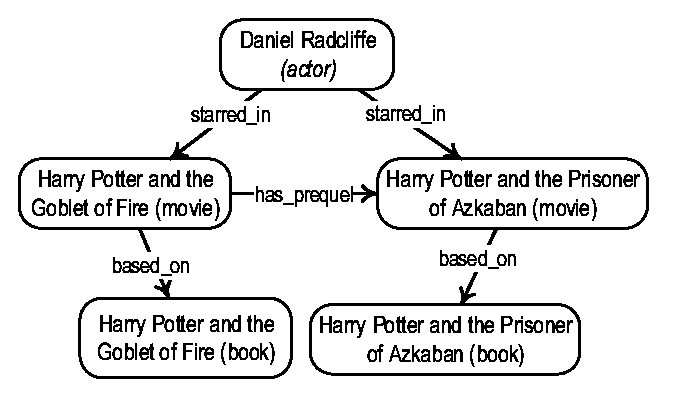
\includegraphics[width=\subfigwidth]{fig/theoretical/example_subgraph_1}\label{fig:context-examples-a}}\\
%         \subfigure[Neighborhood subgraph of size 3 for the entity \textit{Harry Potter}]{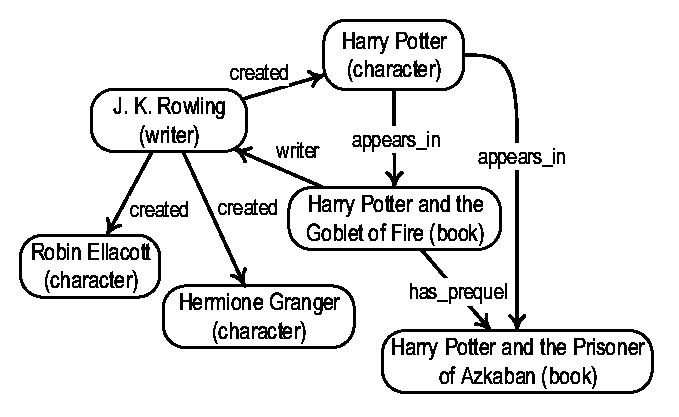
\includegraphics[width=\subfigwidth]{fig/theoretical/example_subgraph_2}\label{fig:context-examples-b}}
%         \caption{Two neighborhood subgraphs for the KG shown in Figure \ref{fig:kg-potter}}
%         \label{fig:context-examples}
%     \end{center}
% \end{figure}

\section{Support and Iterations}
the future of the tool, possible limtations and changes

% \section{Candidates}\label{sec:theo-candidates}
% % As discussed earlier, triples do not make inherent guarantees about the correctness of the knowledge they represent. To represent triples with a higher knowledge quality, this section introduces candidate triples and the notion of fitness in candidate filtering.

% \subsection{Candidate triples}
% % One can form a syntactically correct triple by just combining two random entities with a random relation. However, chances are that the resulting fact is most likely not correct. Contrary to such a low-quality triple, a candidate triple, or just ``candidate'' for short, is a triple that has been created in such a way that its chance to represent correct knowledge is significantly higher than by mere randomness:

% % \defin{Candidate}{
% %     Let $\KG = \KGlong$ be a Knowledge Graph, let $s, t \in \Eset$ be two entities and let $r \in \Rset$ be a relation in \KG. We define a candidate as a triple $(s, r, t)$ that has a significantly high chance to represent real-world knowledge, even if it does not exist in \Tset.
% % }

% % For example, given the KG shown in Figure \ref{fig:kg-potter}, a candidate triple could be \tripleSty{(Daniel Radcliffe, plays, Harry Potter)}. Note that this triple does not exist in the KG in its current state.

% \subsection{Fitness function}
% % Candidate triples can be generated in a wide manner of ways, that we discuss in more detail in the following chapter. However, it is clear that the number of possible triples, in terms of combinations of entities and relations, is generally orders of magnitude greater than the amount of triples present in any given KG. Therefore, it is possible to generate very large sets of candidate triples that are not yet in a KG.

% % As a consequence, it is generally desirable to reduce these sets of candidate triples in a manner that maximizes the preservation of triples with a higher chance to be correct~\cite{shen2022overview, borrego2019}. To formalize this idea, we introduce the concept of fitness function, which assesses the quality of a set of candidate triples in terms of its size and how many correct triples it contains.

% % \defin{Fitness function}{
% %     Let $\KG =$ $\KGlong$ be a Knowledge Graph, let \Sset{} be a set of candidates and let $\Sset'$ be a set of filtered candidates, with $\Sset' \subseteq \Sset$. We define fitness as a function $fitness(\KG, \Sset, \Sset') \rightarrow \mathbb{R}$ that assigns a score to the filtered set of candidates, with respect to the original set of candidates and KG.
% % }

% % Since there are many ways to achieve this, we introduce specific instances of fitness functions in the context of KG completion in Chapter~\ref{chap:chai}.

% \section{Candidate filtering}\label{sec:theo-rule}
% % As previously discussed, it is generally necessary to reduce the size of a set of candidate triples, in order to better assess the remaining candidates for their inclusion in a KG. To achieve this, this section introduces the concept of criterion, and then builds upon it to present the definition of a candidate-filtering rule.

% \subsection{Criterion}
% % A criterion is an atomic element in candidate filtering. Given a candidate triple in the context of a particular Knowledge Graph, a criterion assigns a binary \texttt{False/True} label to the candidate, denoting whether it should be discarded immediately (\texttt{False}), or tentatively accepted and evaluated more carefully (\texttt{True}):

% % \defin{Criterion}{
% %     Let $\KG =$ $\KGlong$ be a Knowledge Graph and let the triple $T = (s, r, t)$ be a candidate for $\KG$. We define a criterion as a function $cr(\KG, T) \rightarrow \{False, True\}$ that assigns a binary label to a candidate triple in the context of a KG.
% % }

% % A given criterion defines a certain method to determine if a candidate triple is likely to be correct or not. For example, a possible criterion would be to accept all candidate triples in which the distance between its two entities is lower than a threshold.

% \subsection{Rule}
% % In order to express more complex manners of filtering candidate triples, we combine several criteria into a rule. A candidate-filtering rule also produces a binary output for a candidate, in this case, by evaluating multiple criteria and combining their results using conjunctions and disjunctions:

% % \defin{Rule}{
% %     Let $\KG =$ $\KGlong$ be a Knowledge Graph, let the triple $T = (s, r, t)$ be a candidate for $\KG$, and let $cr_1,\,cr_2,\,\ldots,\,cr_n$ be a number of criteria. We define a rule as a function $rule(\KG, T) \rightarrow \{False, True\}$ resulting of the conjunction and/or disjunction of several criteria, i.e., $cr_1\,(\wedge | \vee)\,cr_2\,(\wedge | \vee)\,\dots (\wedge | \vee)\,cr_n$.

% % }

% \section{Graph-based features}\label{sec:theo-features}
% % To numerically characterize a triple, we propose a set of graph-based features that takes neighborhood subgraphs, reachable entities and paths into account. Due to the possibly large number of different features that can exist, we also introduce the concept of feature groups. Each group can be parameterized to obtain a specific feature, which we call an instance of the feature group.

% \subsection{Feature}
% % A feature is the simplest way to characterize a triple in the context of the Knowledge Graph it belongs to, by assigning a real number to it according to some operation:

% % \defin{Feature}{
% %     Let $\KG = \KGlong$ be a Knowledge Graph. We define a feature $f$ as a function $f : \Tset \rightarrow \mathbb{R}$ that assigns a real number to a triple.
% % }

% % For example, a feature $f$ may convert a triple into the number of entities in the neighborhood subgraph of size 2 of the source entity, i.e., $f : \triple \mapsto |\Eset{}_s^2|$.

% \subsection{Feature group}
% % Features can have an infinite number of small variations. In our previous example, we mentioned that a feature may leverage the neighborhood subgraph of size 2, but one may conceivably use any subgraph size that is considered appropriate. To be able to express these variations in a more concise way, we define a feature group as follows:

% % \defin{Feature group}{
% %     Let $\KG = \KGlong$ be a Knowledge Graph. We define a feature group $f_n$ as a function $f_n : \fancy{X} \rightarrow (\Tset \rightarrow \mathbb{R})$ that receives a set of parameters \fancy{X} and returns a feature.
% % }

% % % TODO: newpage?
% % For example, a feature group $f_0$ may return a feature that converts a triple into the number of entities in the neighborhood subgraph of size $n$ of the source entity, i.e., $f_0(n) = f : \triple \mapsto |\Eset{}_s^n|$, where $n$ is a parameter of the feature group. Thus, $f_0(2) : \triple \mapsto |\Eset{}_s^2|$, which is the feature shown in the previous example. Consequently, feature groups allow us to represent a set of very similar features in a more compact way, where the only distinction between said features is a given set of parameters.

\section{Summary}\label{sec:framework-summary}
% In this chapter, we have described the conceptual framework our proposal relies on. We have defined Knowledge Graphs, triples, paths, distance in a KG and reachability. Furthermore, we have introduced neighborhood subgraphs, candidate triples and fitness functions, as well as candidate-filtering criteria and rules. Finally, we have described graph-based features and their groups.

    %%%%%%%%%%%%%%%%%%%%%%%%%%%%%%%%%%%%%%%%

    \part{Final Remarks}
    \chapter{Conclusions}\label{chap:conclusions}

% guarrada para que las dos líneas queden más o menos alineadas sin contar las comillas, sorry
\chapterQuote{\hfill\textit{``Some peoples only exercise is jumping to conclusions.''}}{--- \textit{Author Unknown.}}

\vspace{1cm}

In this dissertation, we have presented SpaceRL a framework offering a set of reinforcement learning tools tailored towards Knowledge Graph completion and reasoning; a versatile tool with different available interfaces, a visualization tool to graphically display the results, a GUI  that provides access to less experienced users, and a REST API that enables for it to be operated as a MLaaS.

SpaceRL was designed not only as a tool for final users, but also as a base for other developers to create their own custom tools, which can be offered as a service to a third party through its API complying with the openAPI convention. This might appeal to companies who wish to either serve or consume the capabilities offered.

Other existing proposals have merely scratched the surface when it comes to reward functions, applying unanimously terminal-based reward functions with minimal modifications and the backpropagation-focused REINFORCE algorithm in tandem.

Our novel alternative consists of a new set of reward functions and the application of RL algorithms whose potential remained unexplored. Our reward functions seek to use graph-specific information that is available before reaching the end of an episode: the distance to the answer node, and the semantic similarity to it computed from node embeddings. The implemented technique makes use of Proximal Policy Optimization and the Actor-Critic paradigm, resulting in faster training.

Both the new reward functions and policies have resulted in improvements over the state-of-the-art standard practices, particularly when using embedding-based reward functions on five widely used datasets. These results should motivate the development and evaluation of more variants of these aspects, since there is margin for improvement. Therefore, two trends of future work could be developed: 1) evaluating existing context-independent RL techniques, which are often already implemented by existing libraries but mainly remain untested in this context; 2) implementing new reward functions that make use of additional information in the graph, e.g. node attributes, which provide additional rich data.

    %%%%%%%%%%%%%%%%%%%%%%%%%%%%%%%%%%%%%%%%

    % Bibliografía
    \bibliographystyle{abbrvnat}
    \bibliography{bibliography.bib}
    
\end{document} 